%-------------------------------
%-------------------------------
\chapter{PCA Daten}
\label{appendix_pca}

%-----------------------------
\section{Eingabedaten für PCA}

%- - - - - - - - - 
\subsection{Bilder}
\label{picture_sources}
 
 Alle Bilder, die als Eingabe für die PCA verwendet wurden, sind in Abbildung \ref{all_images} zu finden. Im Folgenden sind die Bildquellen aufgezählt.
 Alle Tiere, die nicht aufgezählt sind, sind aus \cite{Spezielle_Zoologie} entnommen.
 \begin{itemize}
  \item Archaeopteryx, Eusthenopteron, Ichthyosaurus, Ichthyostega, Muraenosaurus, Urpferdchen aus \cite{Zoologie24Wehner}
  \item Blauwal \url{https://www.quagga-illustrations.de/wp-content/uploads/2014/05/h0001705.jpg}
  \item Chamäleon \url{https://www.madcham.de/de/anatomie/}
  \item Dormedar \url{https://upload.wikimedia.org/wikipedia/commons/a/ac/Camel_Skeleton_-_Richard_Owen_-_On_the_Anatomy_of_Vertebrates_\%281866\%29.jpg}
  \item Giraffe\\ \url{https://de.wikipedia.org/wiki/Giraffen#/media/Datei:Giraffe_skeleton.jpg}
  \item Gnu \url{https://lutzmoeller.net/Afrika/2007/Lutz-Juli/8-Gnu.php}
  \item Känguru \url{http://www.bildwoerterbuch.com/tierreich/beuteltiere/kaenguru/skelett-eines-kaengurus.php}
  \item Krokodil \url{https://de.depositphotos.com/210906852/stock-illustration-skeleton-crocodile-vintage-line-drawing.html}
  \item Pferd \url{https://www.kosmos.de/content/buecher/ratgeber/pferde-reiten/vorwaerts-abwaerts-eine-frage-der-haltung/}
  \item Schlange: zu Schlangen gibt es keine Bilder, die deren Skelett in ausgestrecktem Zustand von der Seite darstellen. Deshalb wurde ein leeres Bild genommen und der Verlauf des Rückens durch eine Gerade angenähert (Extremitäten besitzt eine Schlange nicht. Außerdem ist nicht erkennbar ob \bzw wo Hals in Rücken und Rücken in Schwanz übergeht. Deshalb wurde die komplette Wirbelsäule als Rücken markiert.)
  \item Schwan \url{https://www.alamy.de/skelett-eines-schwans-osteographia-oder-die-anatomie-der-knochen-london-1733-quelle-47-ich-12-kapitel-v-saitenhalter-autor-cheselden-william-image226921369.html}
  \item Seekuh aus \cite{Zoologie25Wehner}
  \item Sinornis und Taube aus \cite{Vergleichende_Anatomie}
  \item Strauß \url{https://www.alamy.de/stockfoto-skelett-von-strauss-24658845.html}
  \item Tyrannosaurus Rex \url{https://upload.wikimedia.org/wikipedia/commons/9/9f/Tyrannosaurus_skeleton.jpg}
 \end{itemize}
 
\begin{figure}
\subfloat[Afrikanischer Elefant]{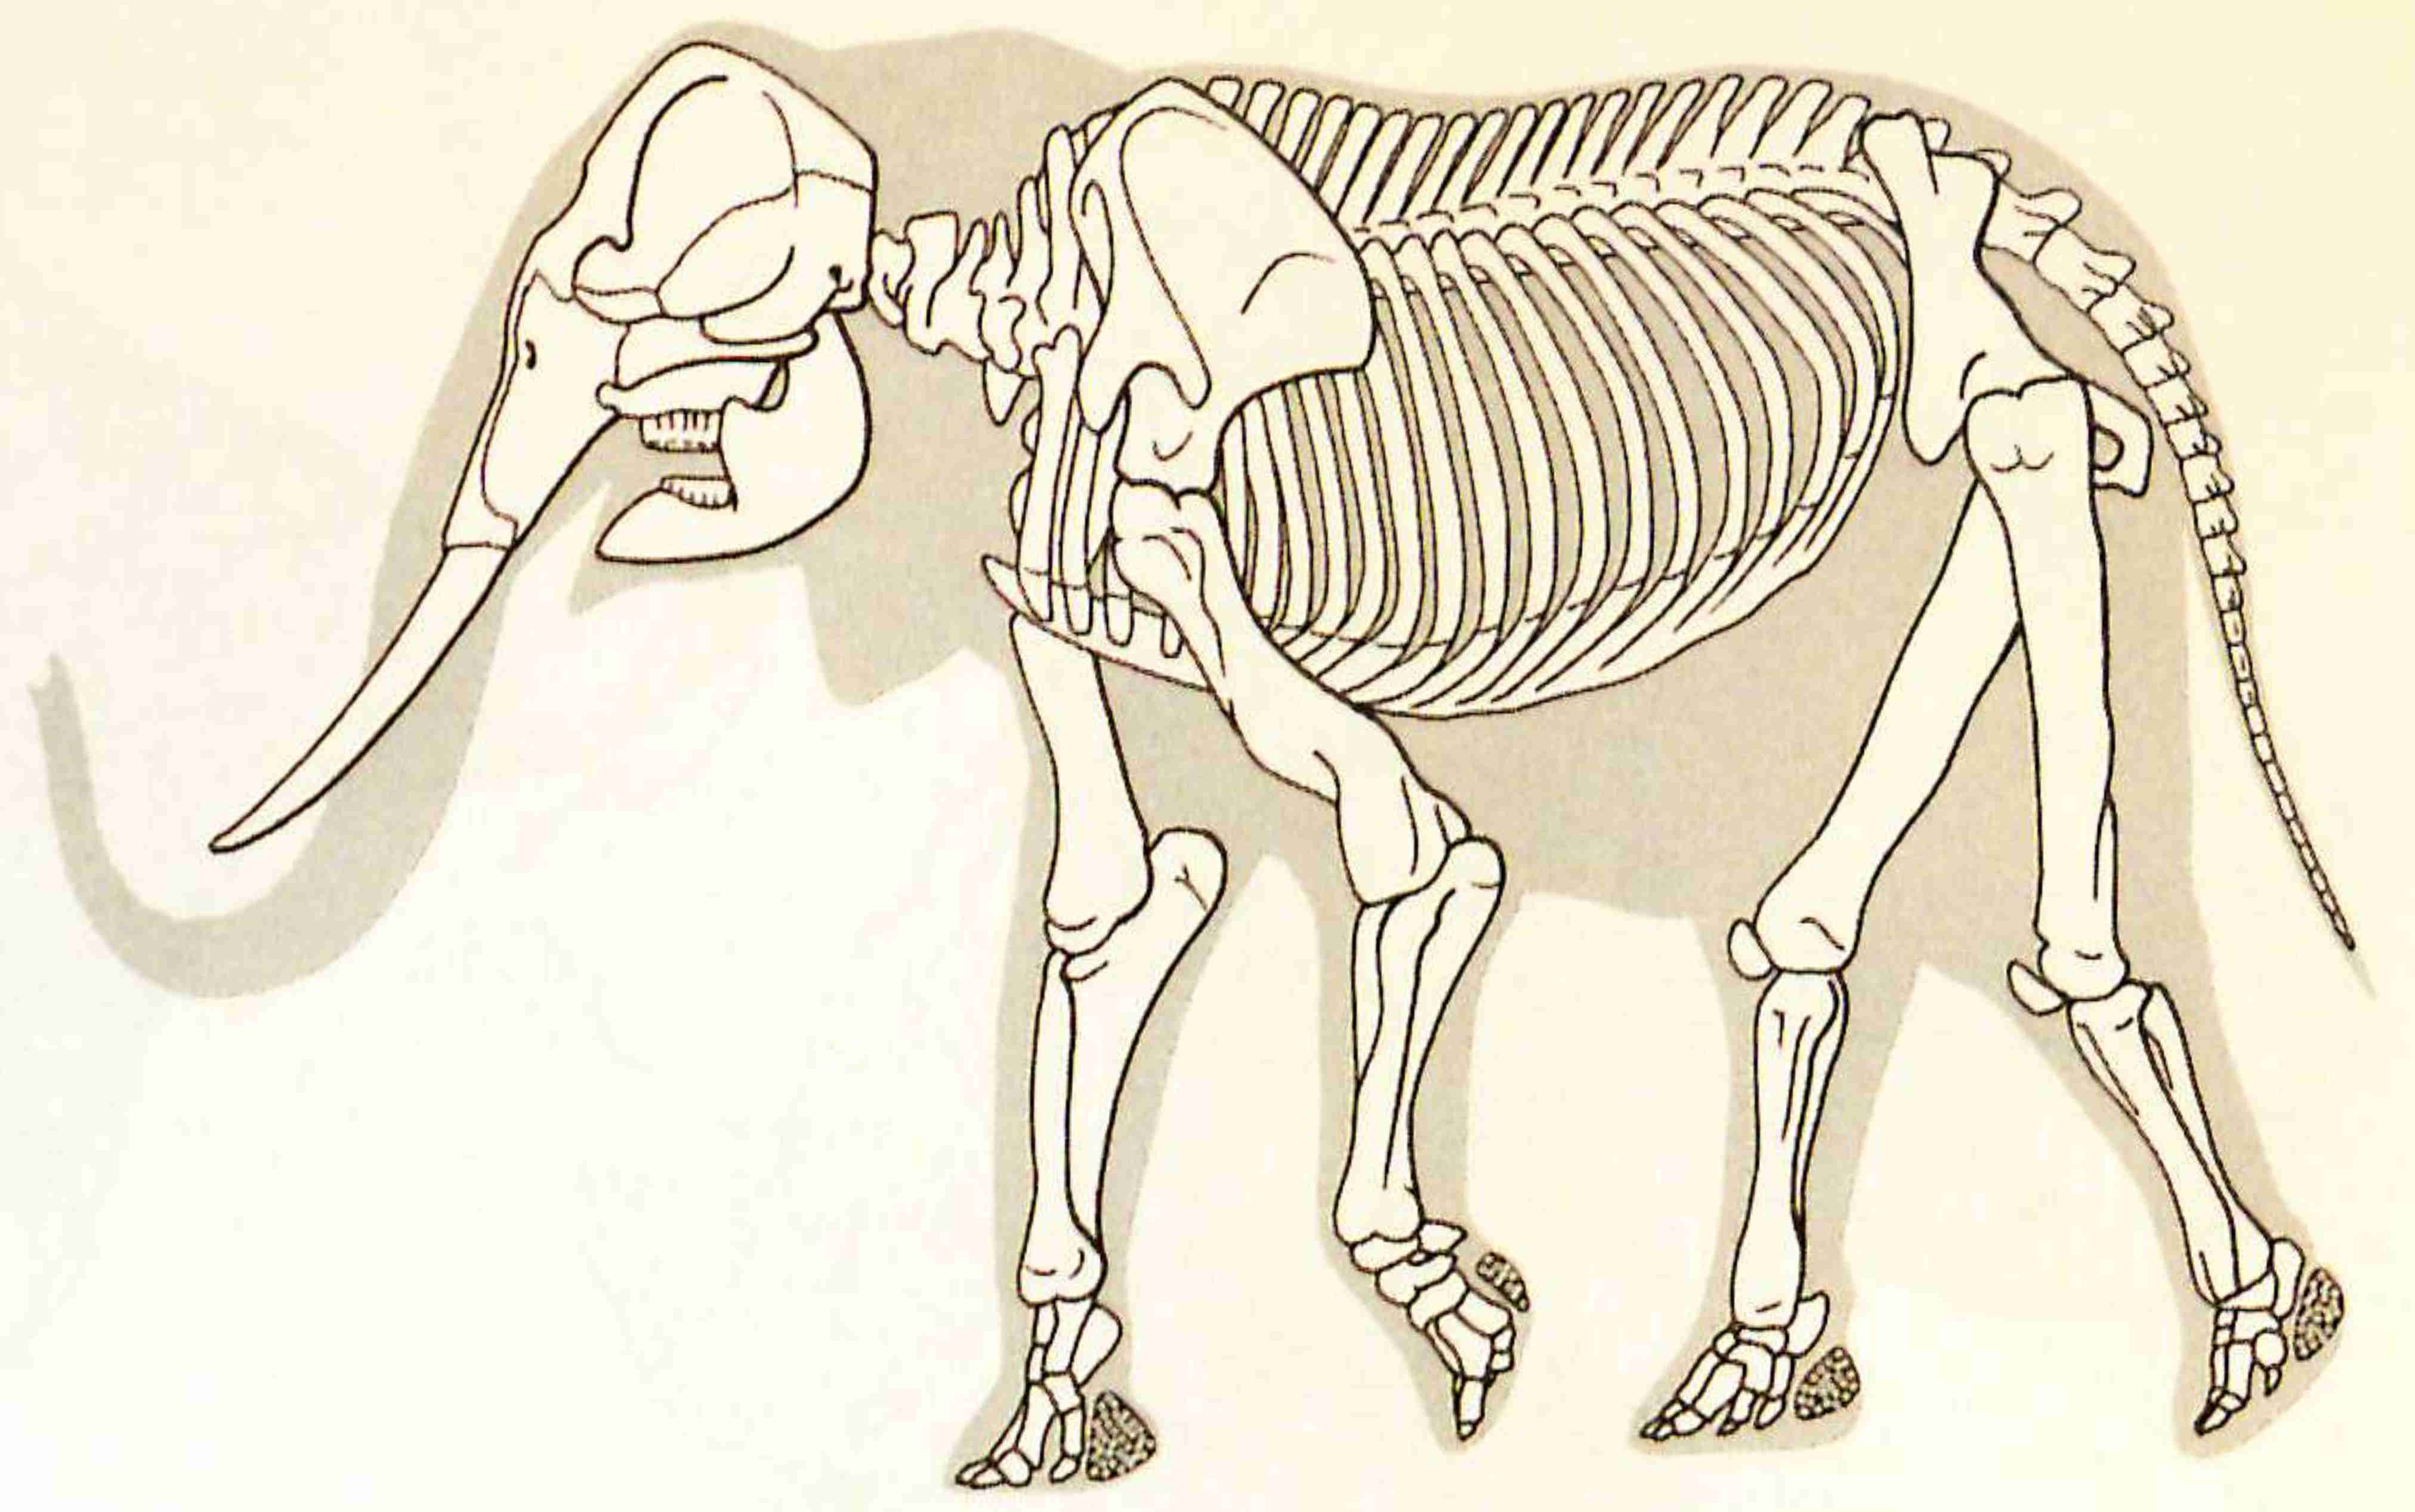
\includegraphics[width=0.2\textwidth]{../PCA/Skelettbilder_klein/Afrikanischer_Elefant.jpg}}~
\subfloat[Amerikanischer Flussbarsch]{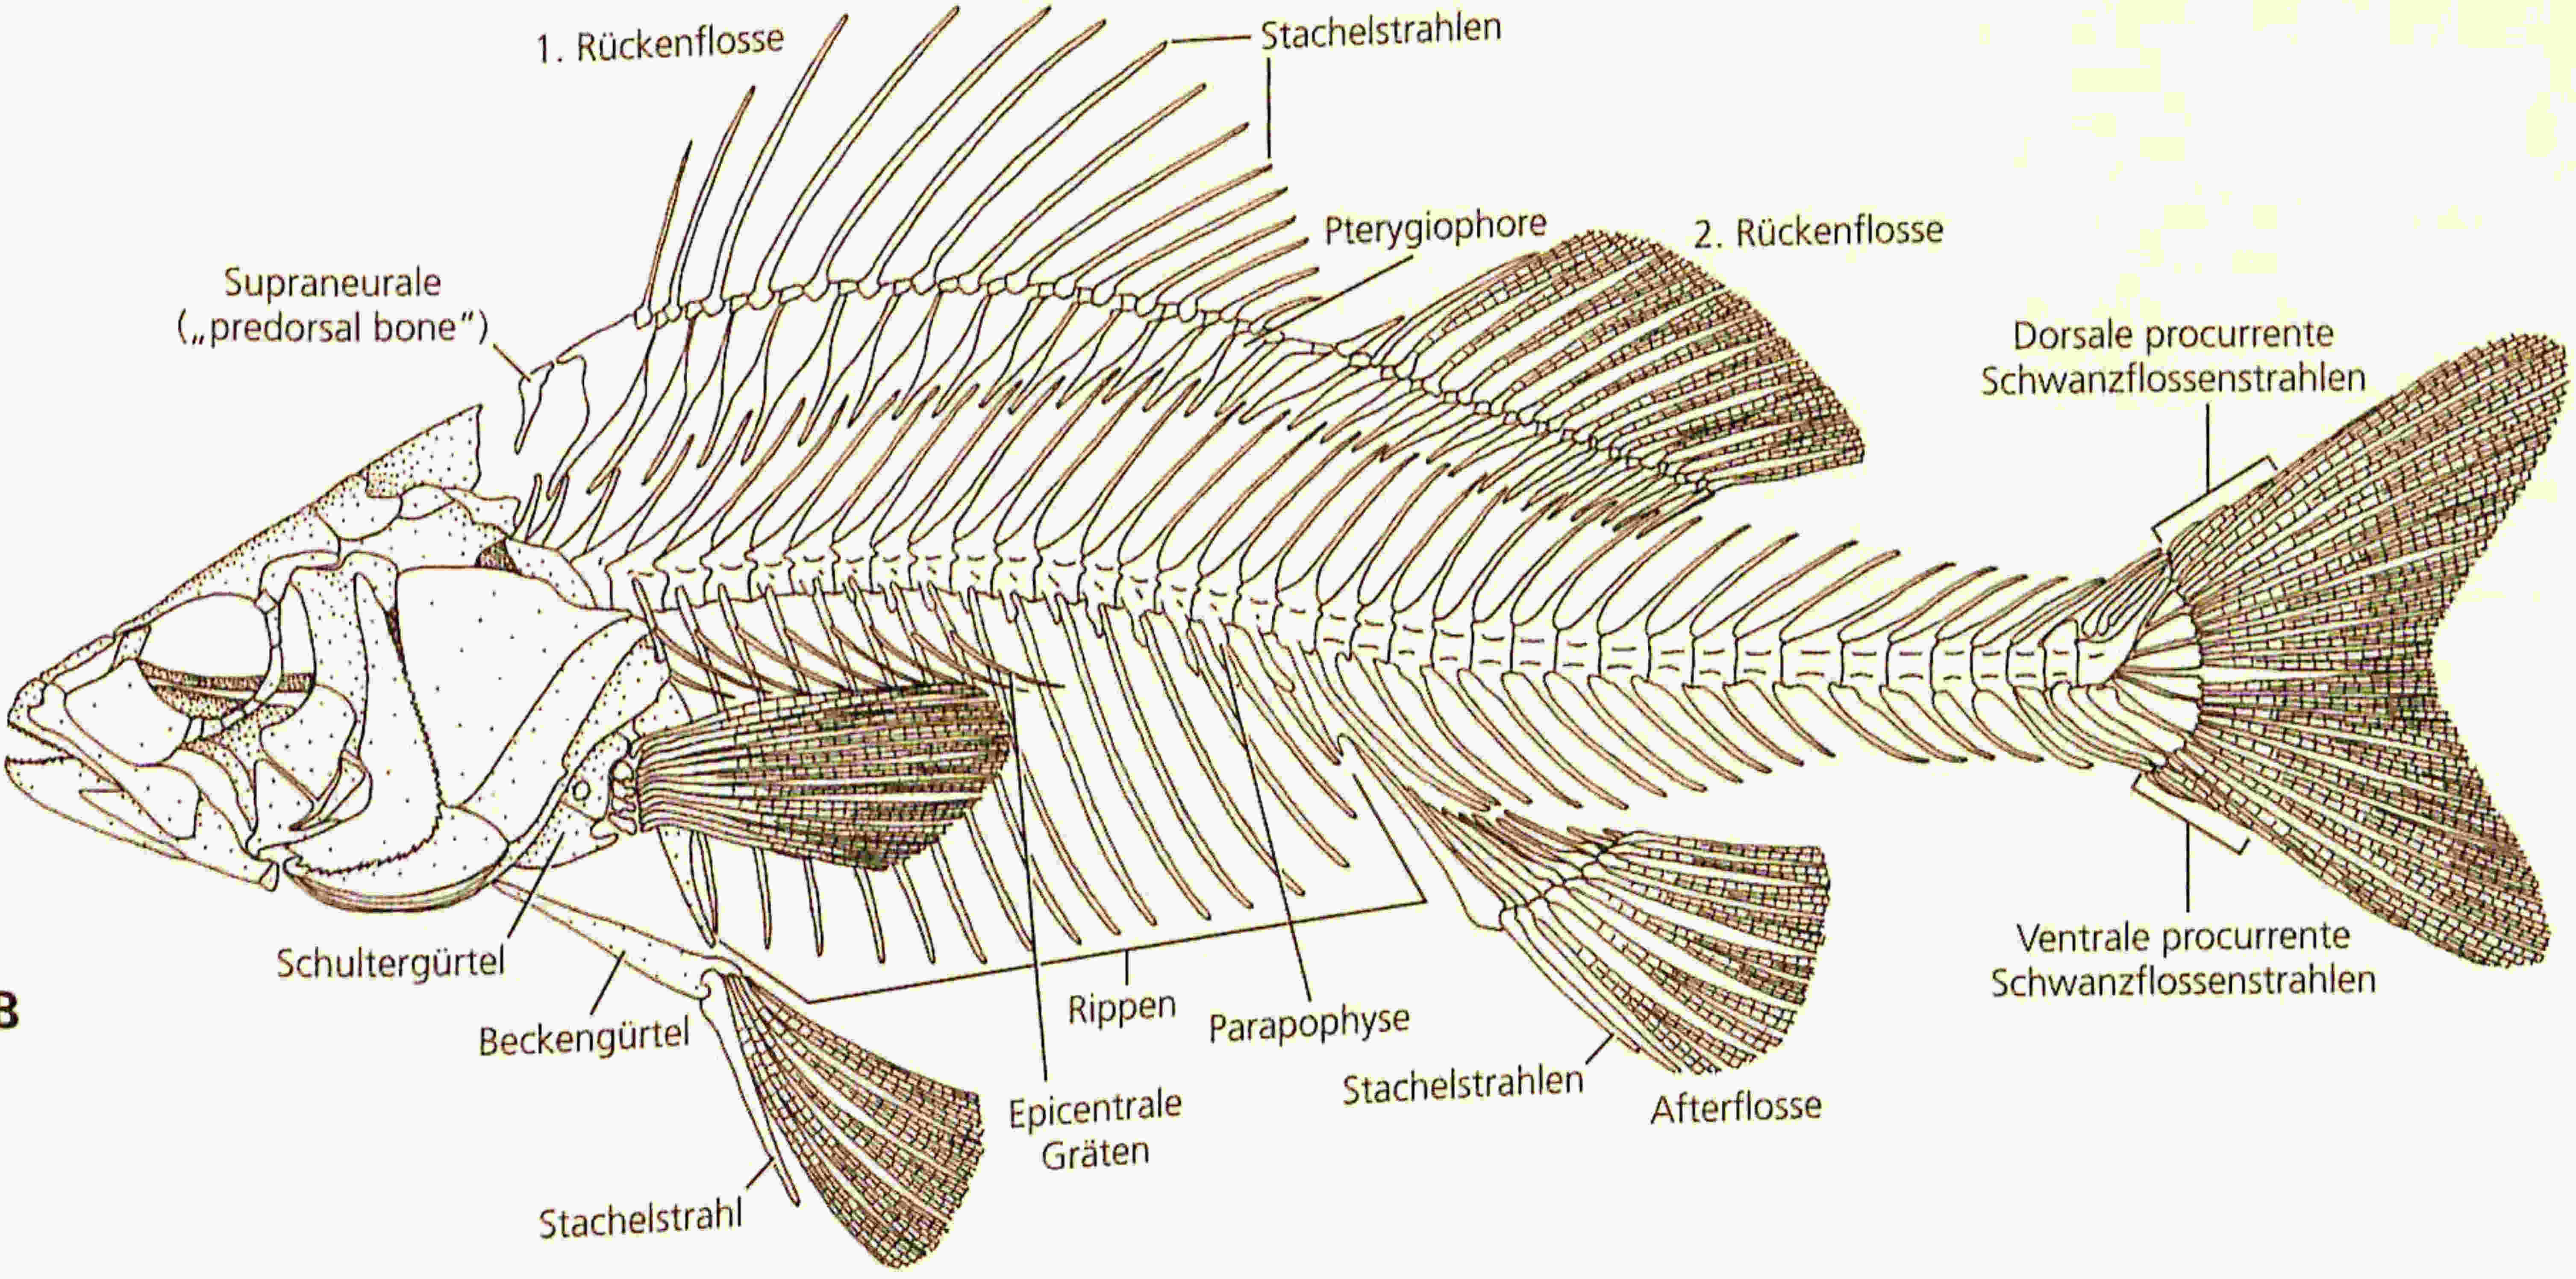
\includegraphics[width=0.2\textwidth]{../PCA/Skelettbilder_klein/Amerikanischer_Flussbarsch.jpg}}~
\subfloat[Archaeopteryx]{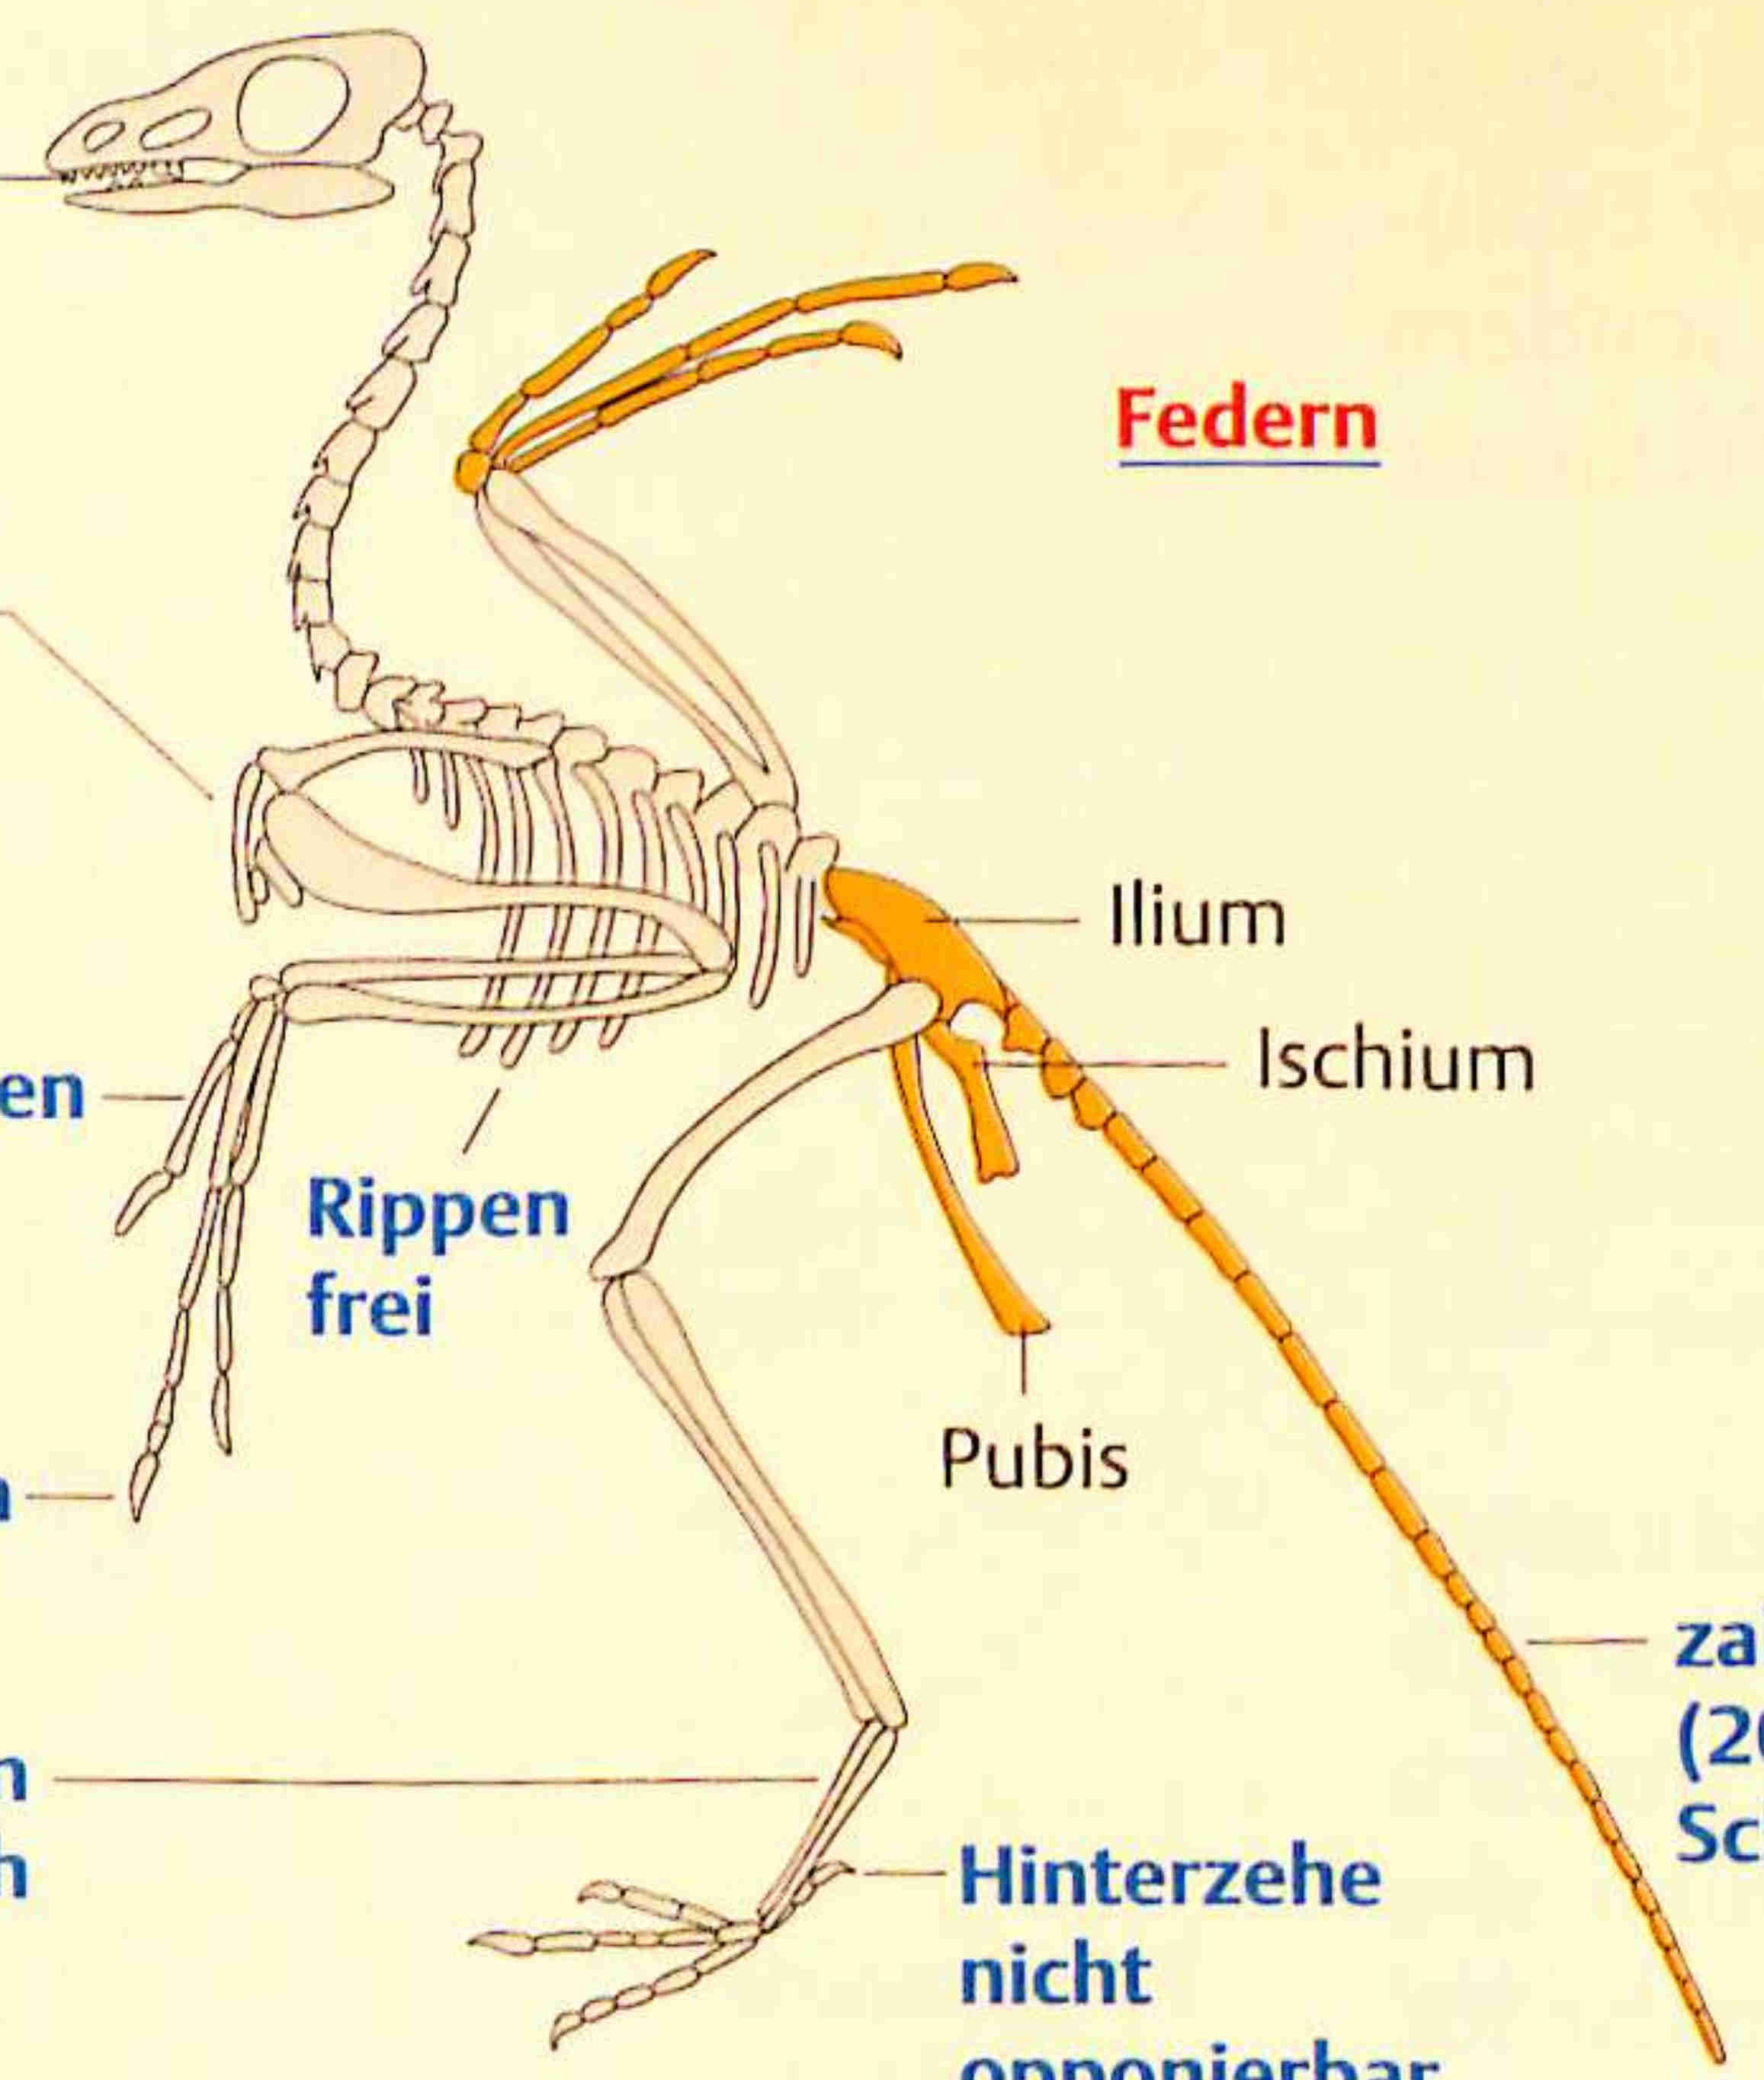
\includegraphics[width=0.2\textwidth]{../PCA/Skelettbilder_klein/Archaeopteryx.jpg}}~
\subfloat[Blauwal]{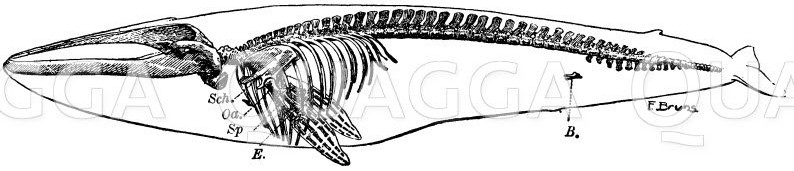
\includegraphics[width=0.2\textwidth]{../PCA/Skelettbilder_klein/Blauwal.jpg}}~
\subfloat[Brachiosaurus]{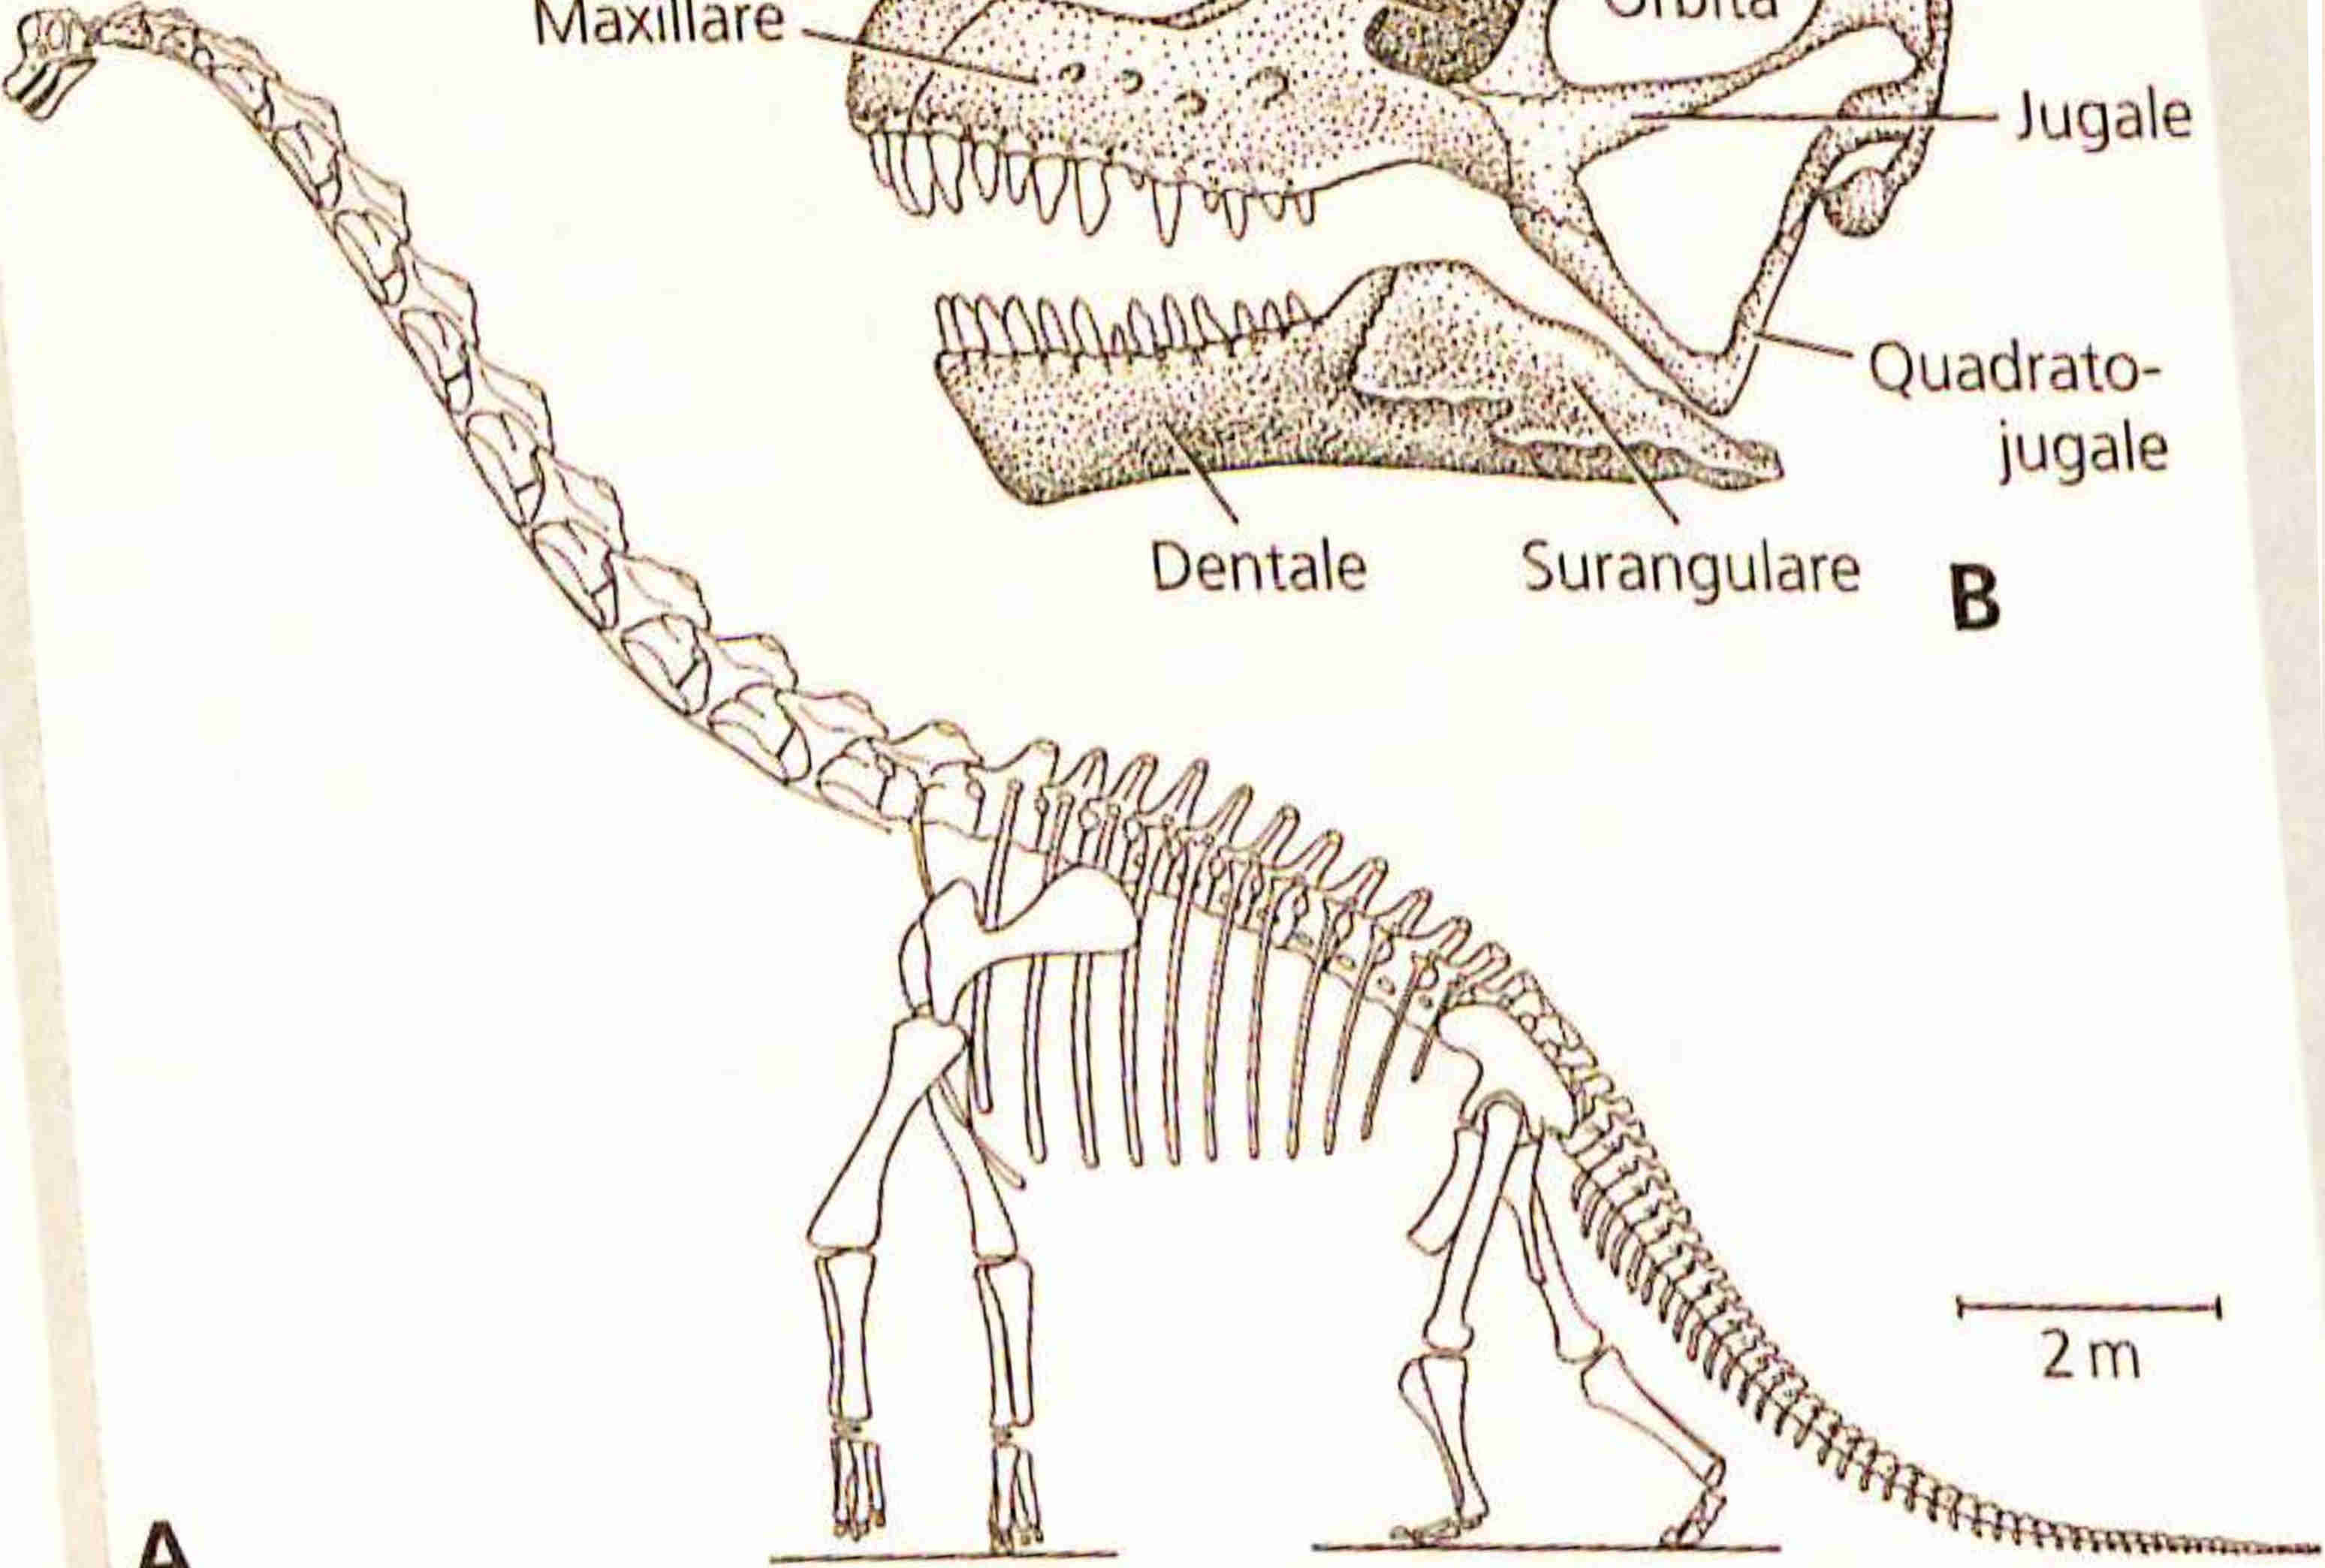
\includegraphics[width=0.2\textwidth]{../PCA/Skelettbilder_klein/Brachiosaurus.jpg}}
\\
\subfloat[Chamaeleon]{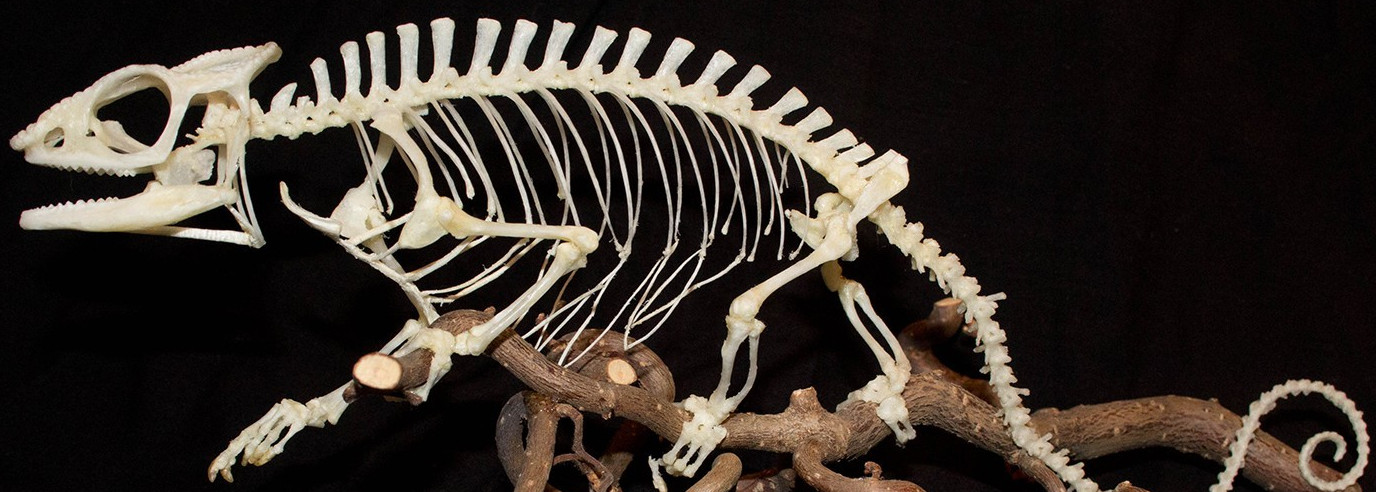
\includegraphics[width=0.2\textwidth]{../PCA/Skelettbilder_klein/Chamaeleon.jpg}}~
\subfloat[Dimetrodon]{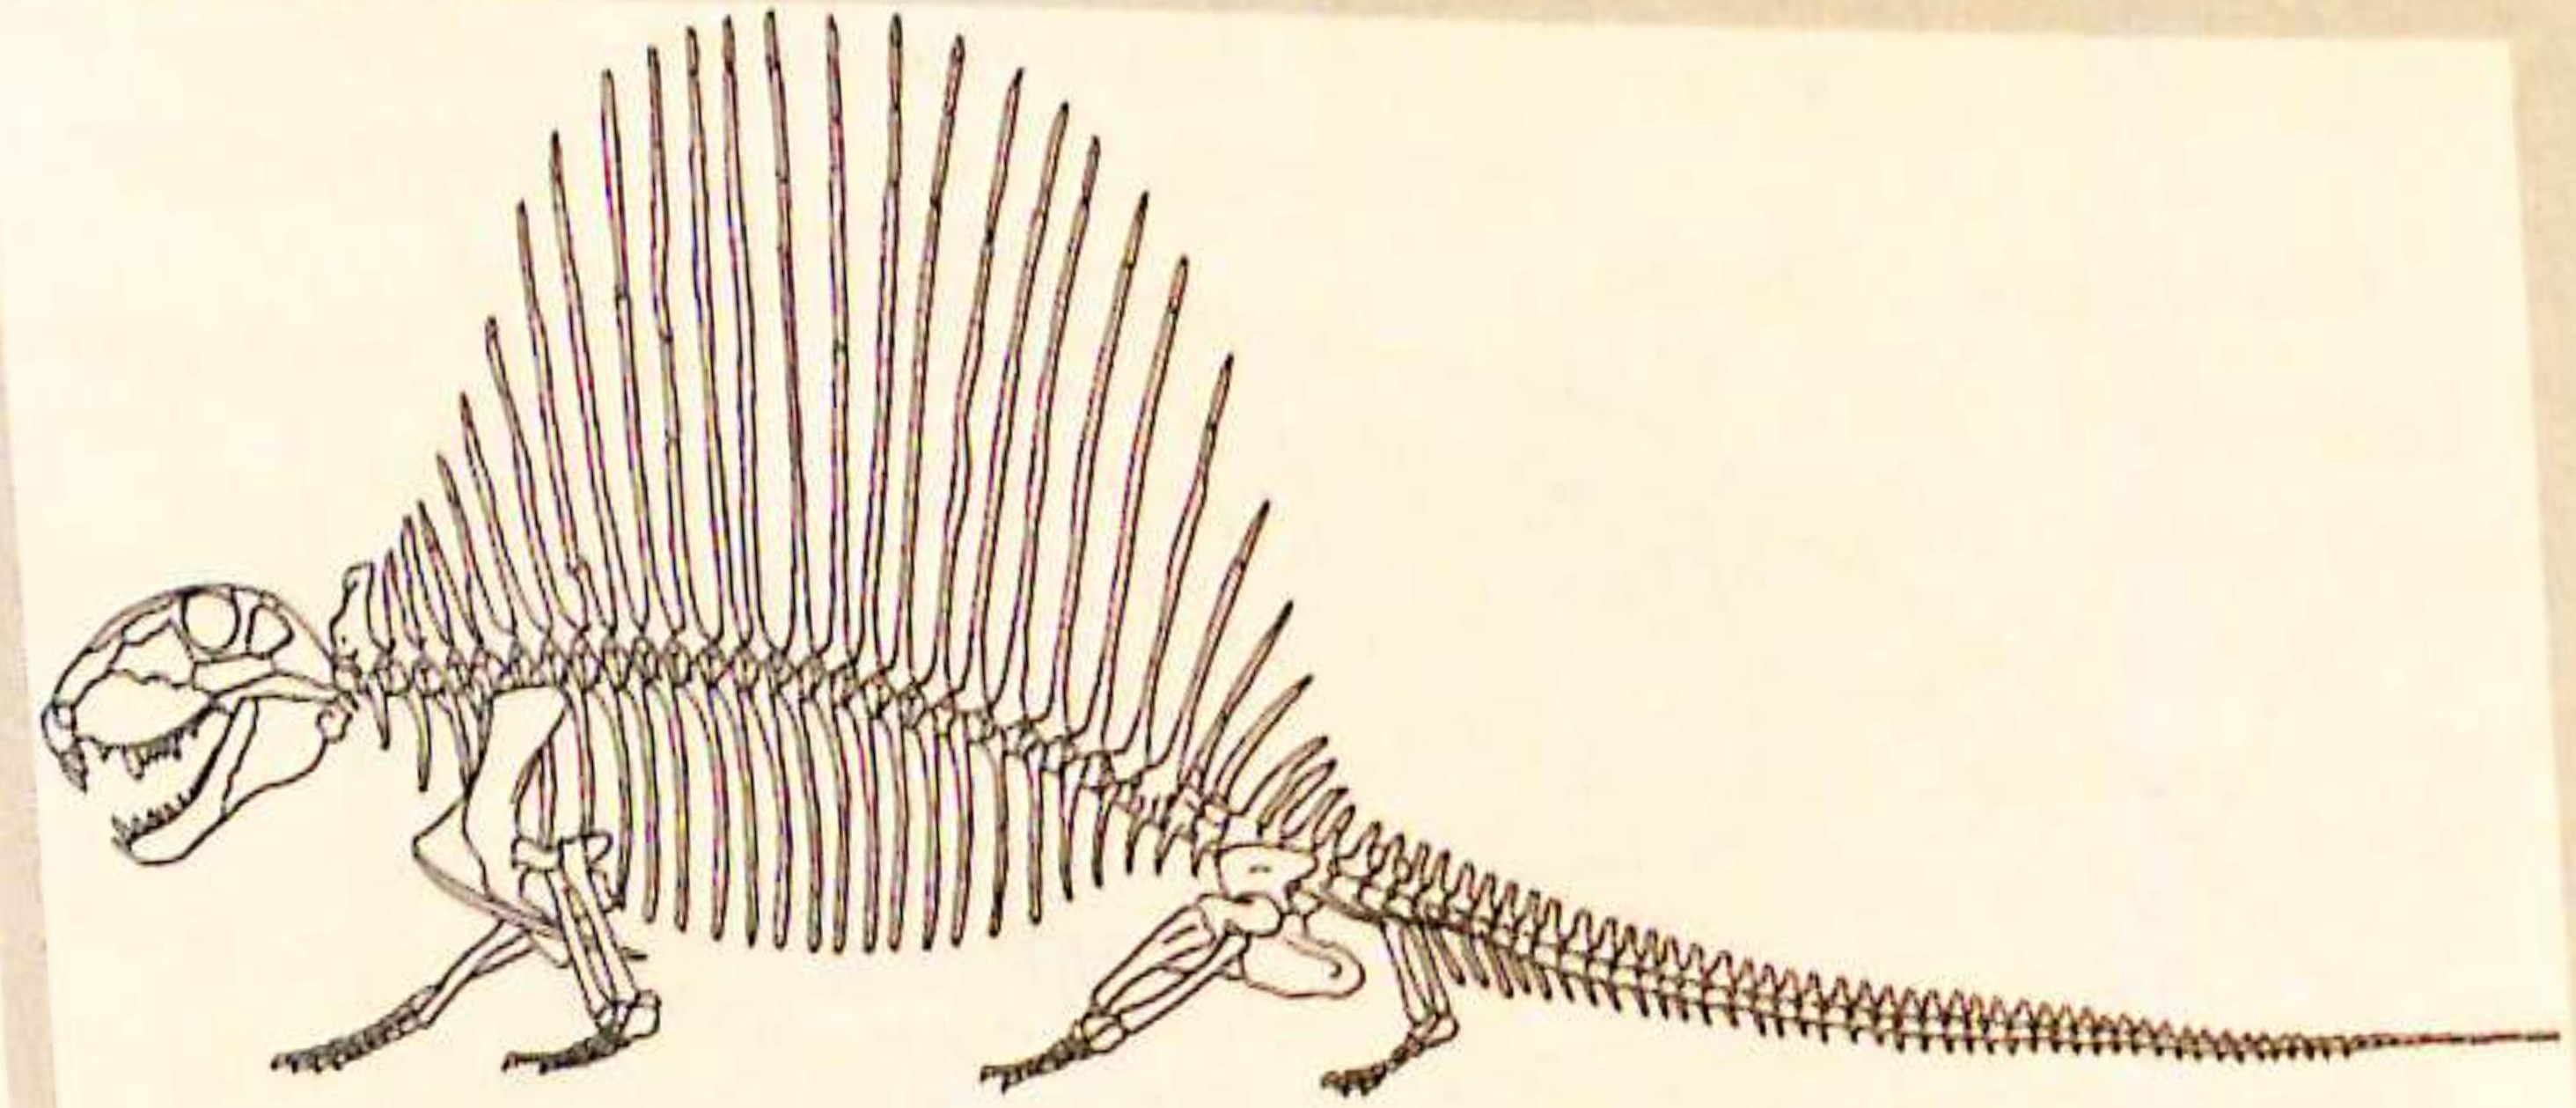
\includegraphics[width=0.2\textwidth]{../PCA/Skelettbilder_klein/Dimetrodon.jpg}}~
\subfloat[Dromedar]{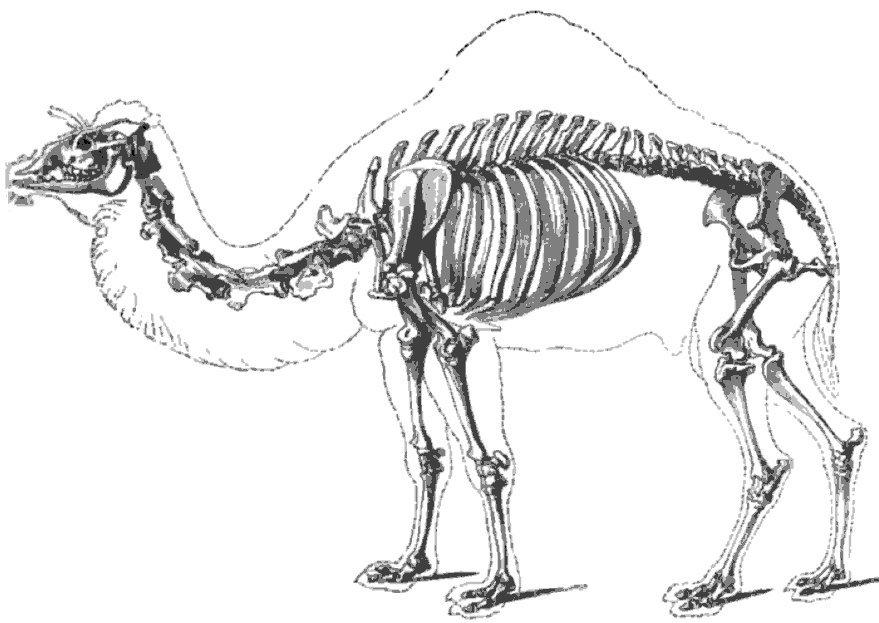
\includegraphics[width=0.2\textwidth]{../PCA/Skelettbilder_klein/Dromedar.jpg}}~
\subfloat[Elster]{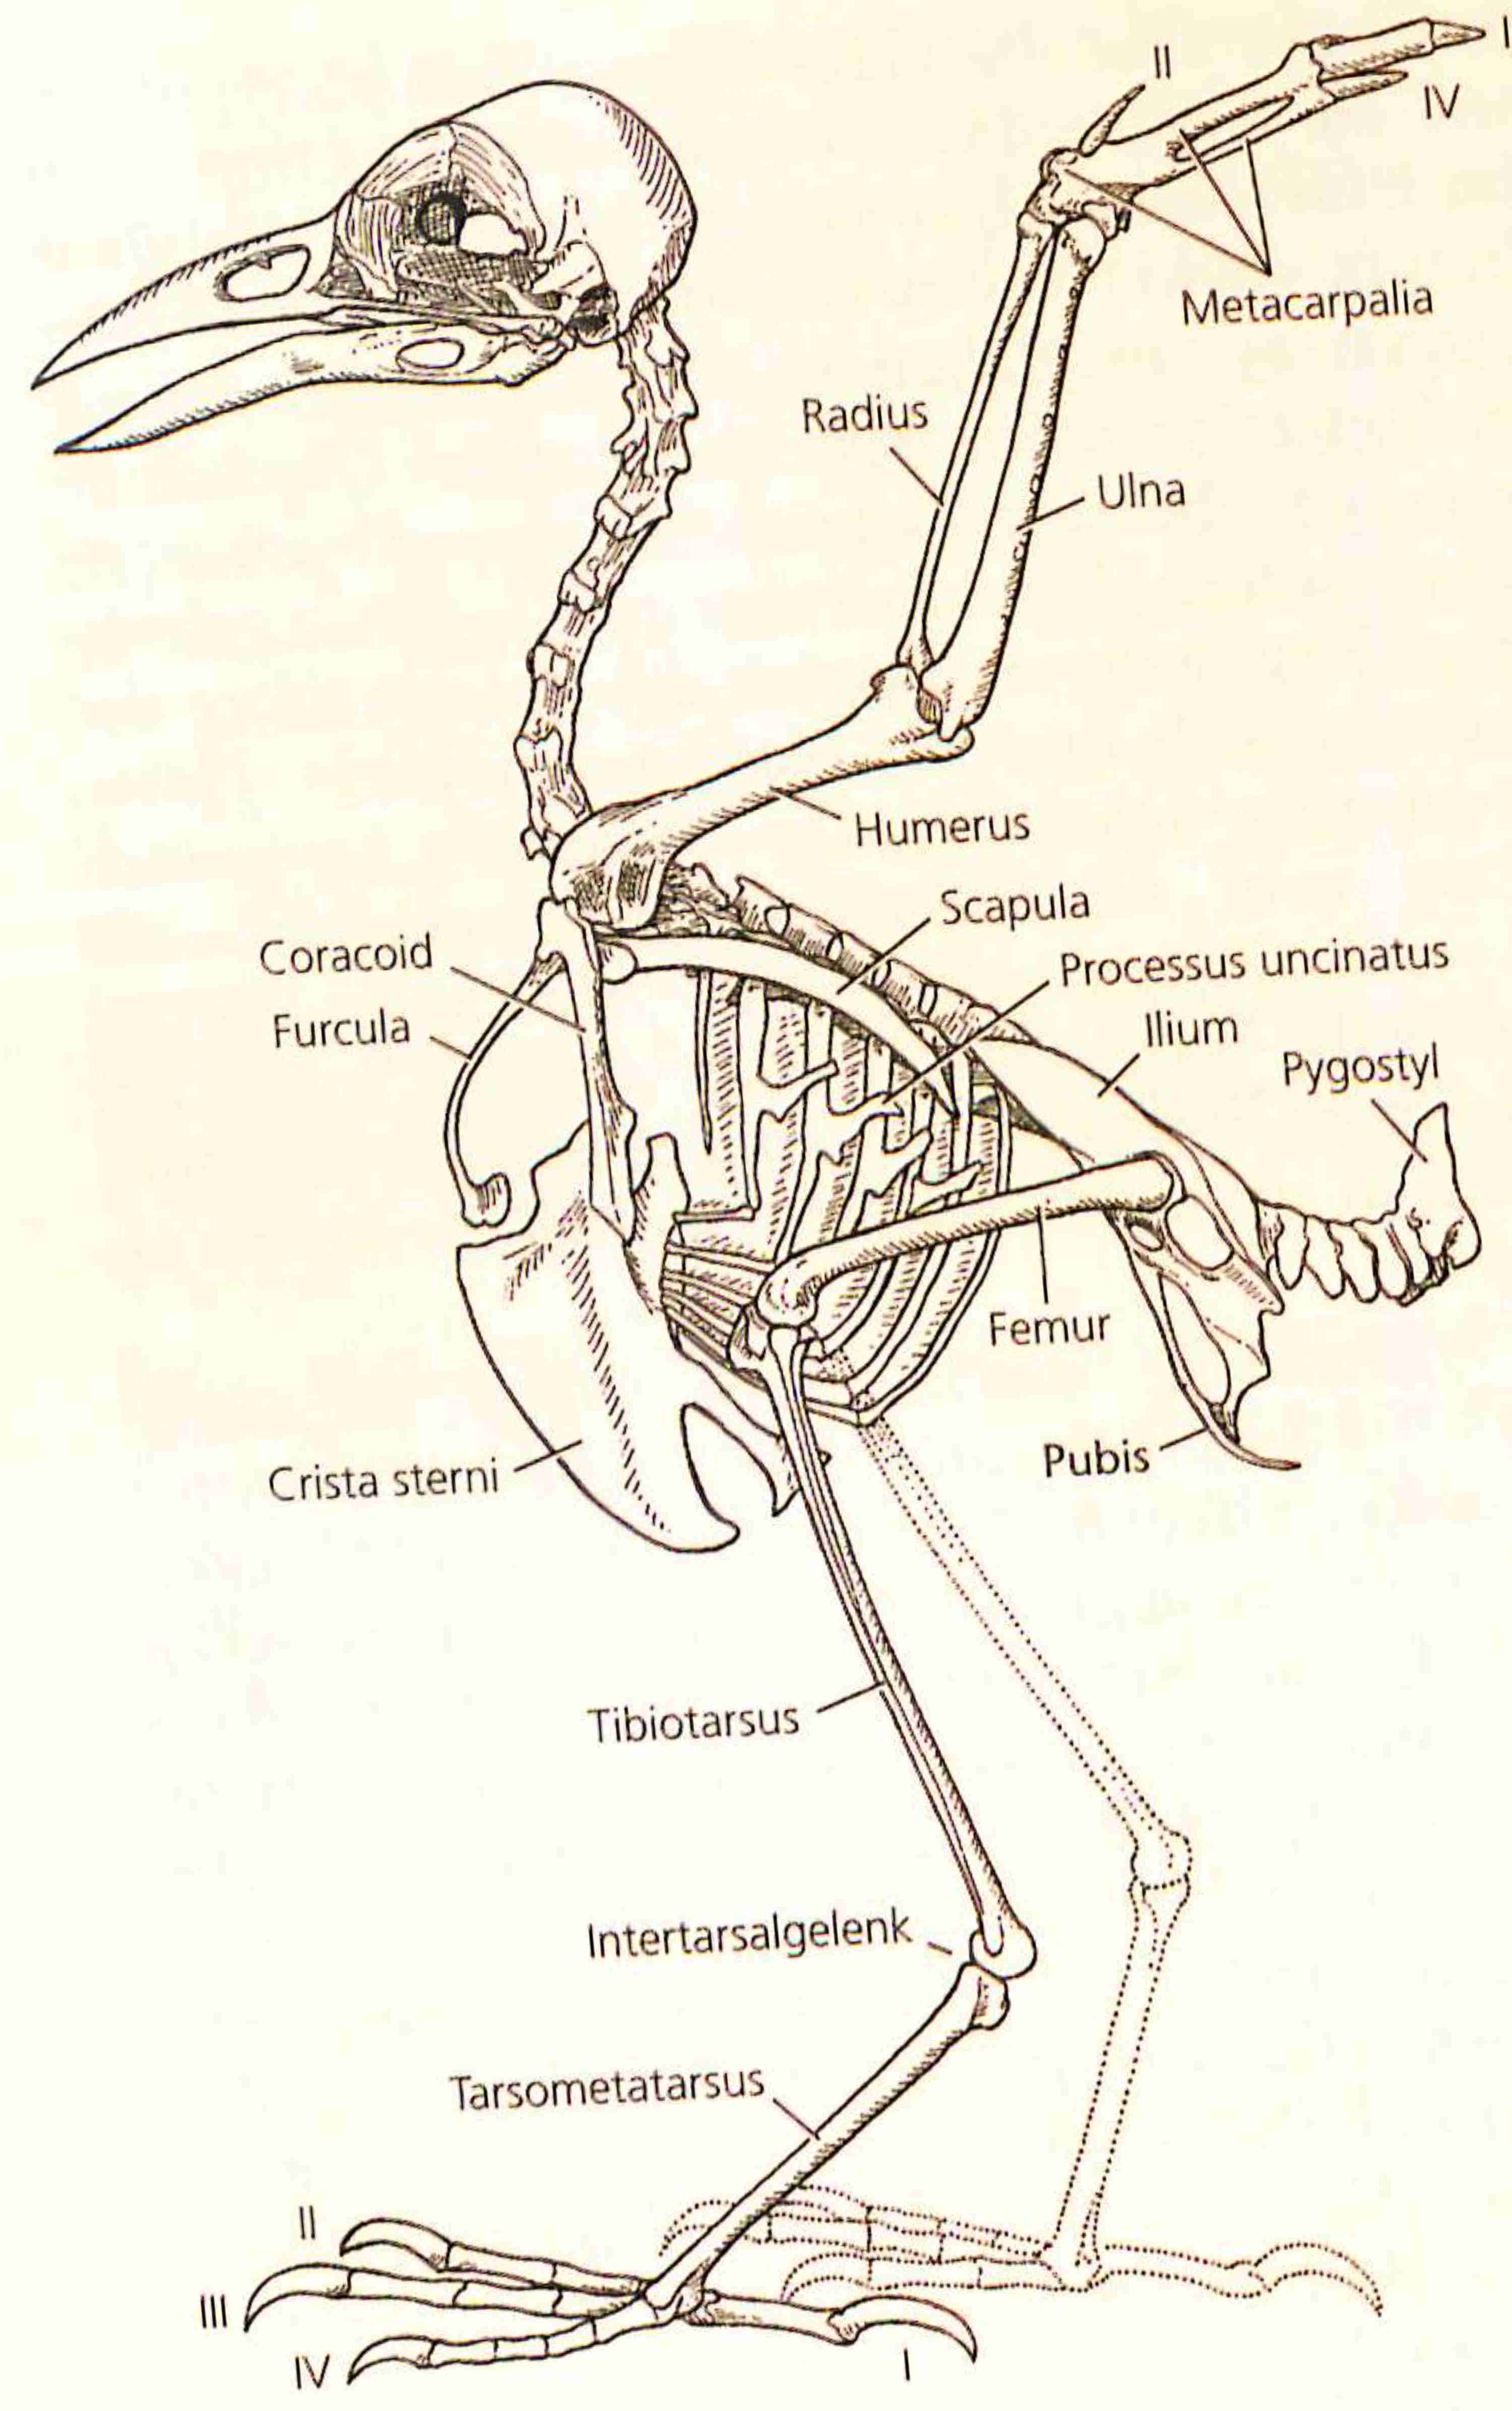
\includegraphics[width=0.2\textwidth]{../PCA/Skelettbilder_klein/Elster.jpg}}~
\subfloat[Forelle]{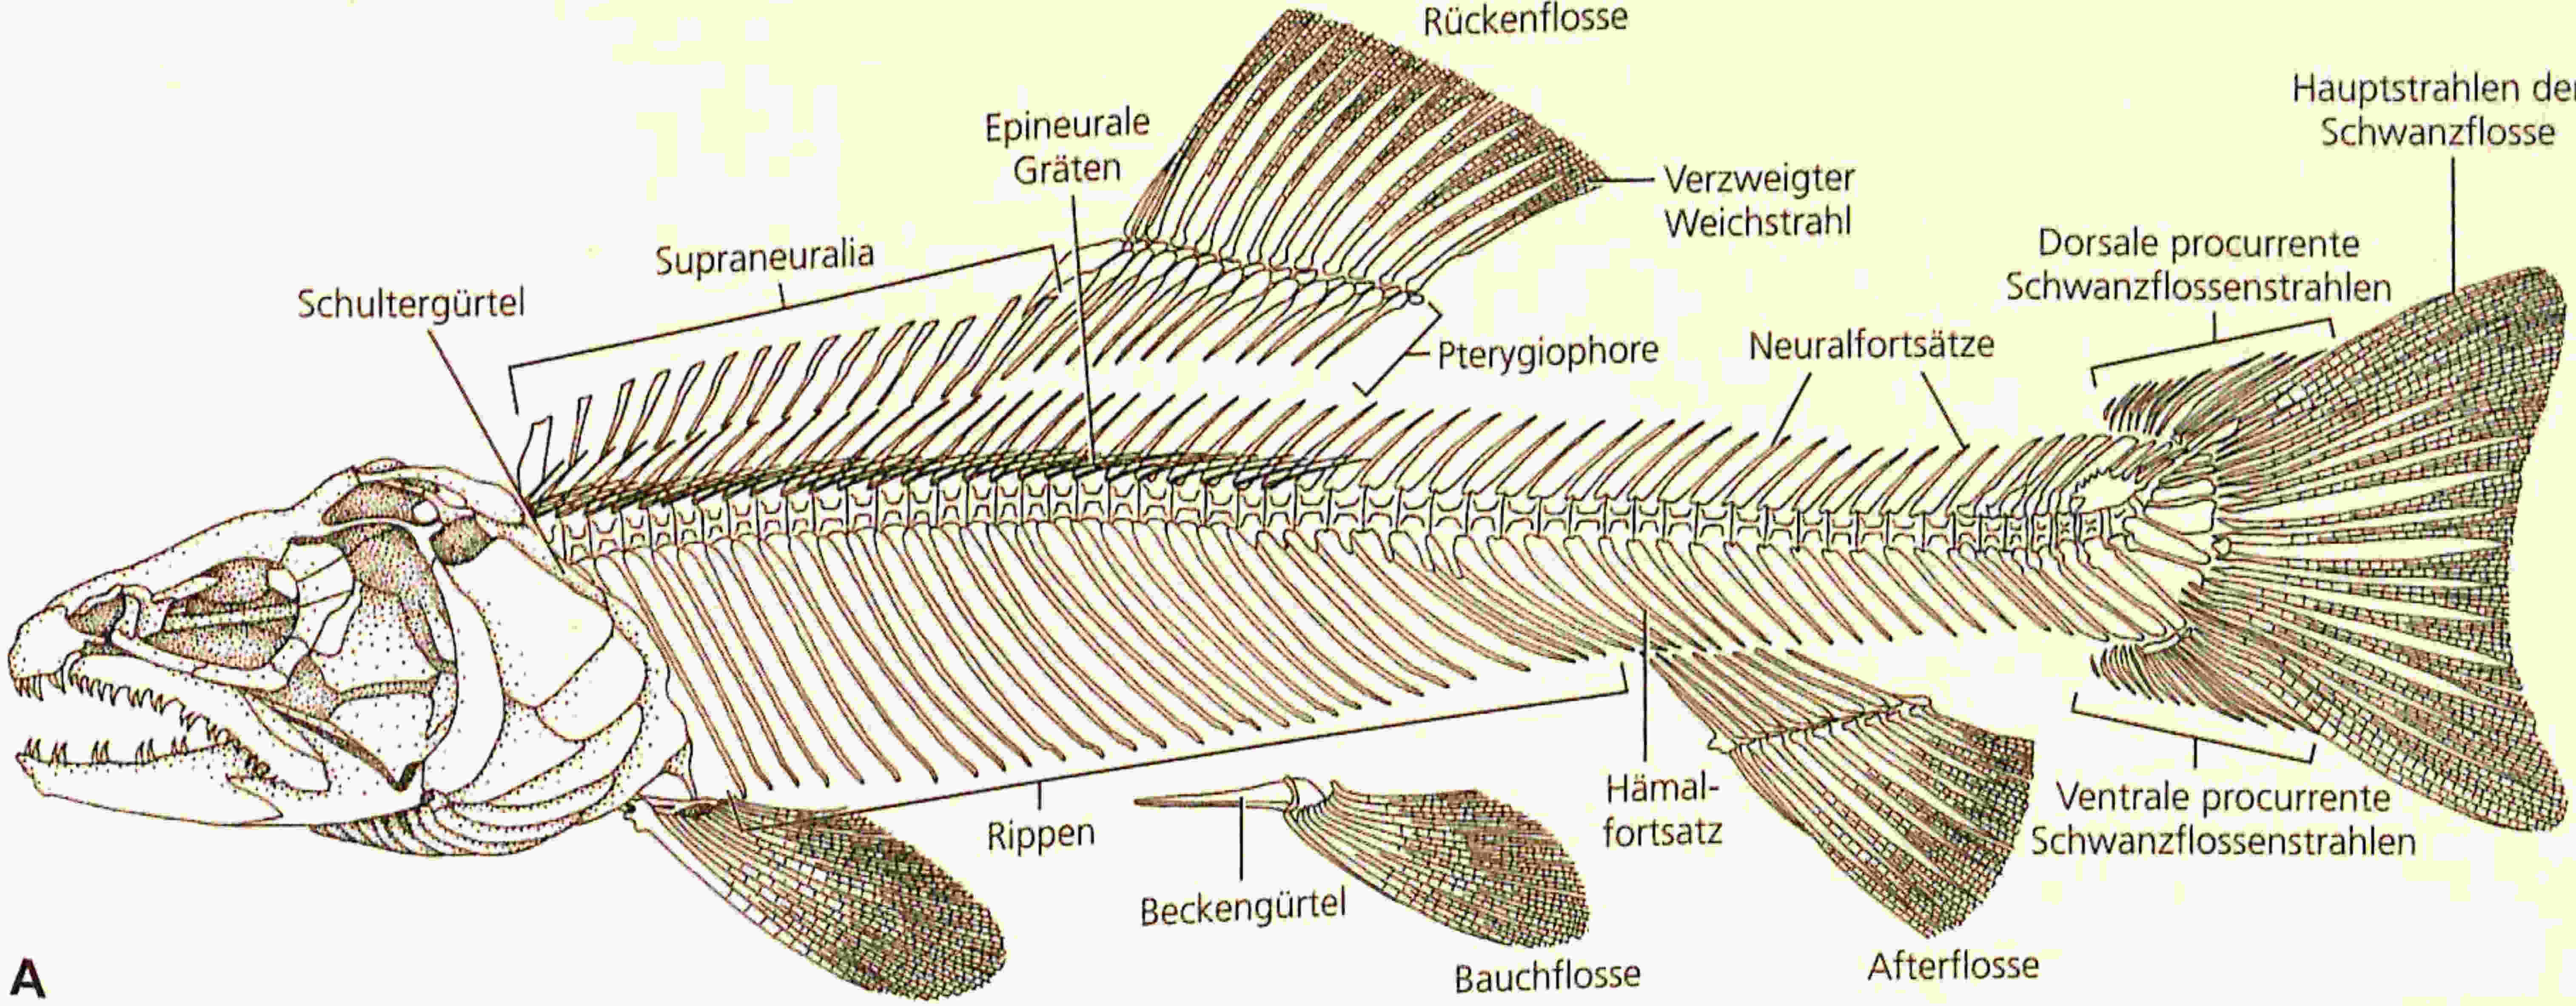
\includegraphics[width=0.2\textwidth]{../PCA/Skelettbilder_klein/Forelle.jpg}}
\\
\subfloat[Frosch]{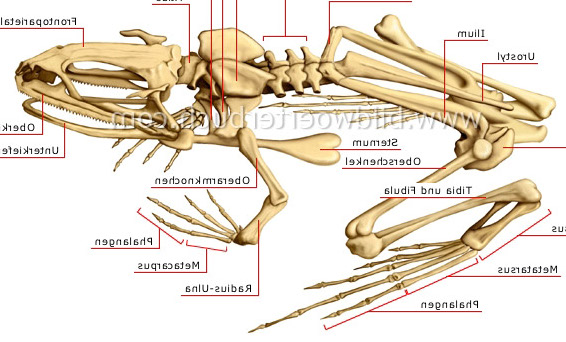
\includegraphics[width=0.2\textwidth]{../PCA/Skelettbilder_klein/Frosch.jpg}}~
\subfloat[Gaemse]{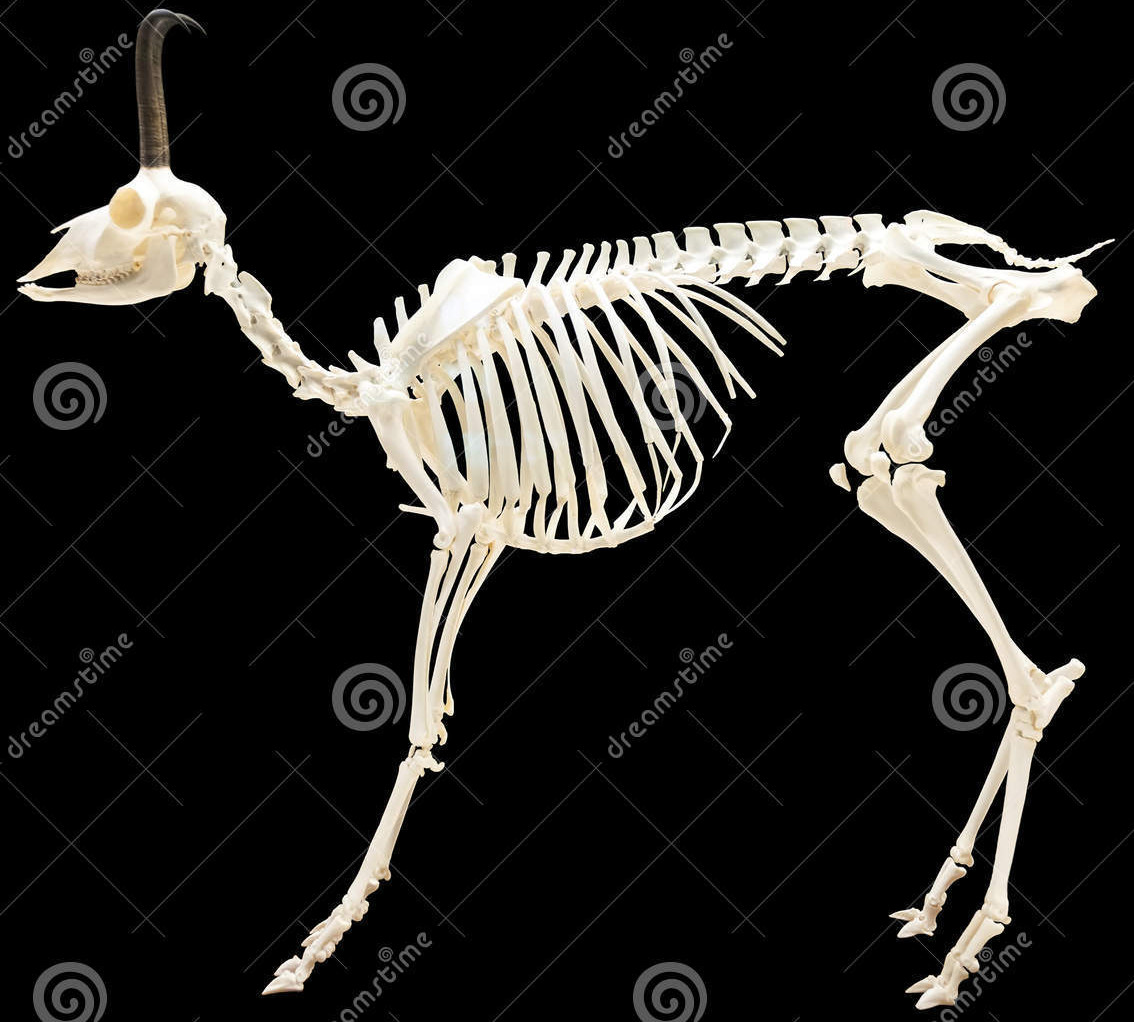
\includegraphics[width=0.2\textwidth]{../PCA/Skelettbilder_klein/Gaemse.jpg}}~
\subfloat[Giraffe]{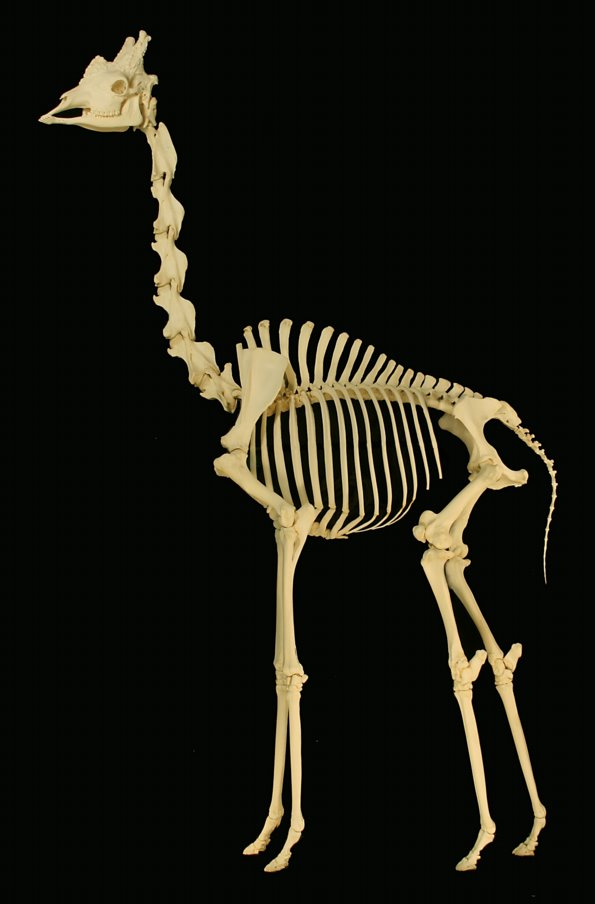
\includegraphics[width=0.2\textwidth]{../PCA/Skelettbilder_klein/Giraffe.jpg}}~
\subfloat[Gnu]{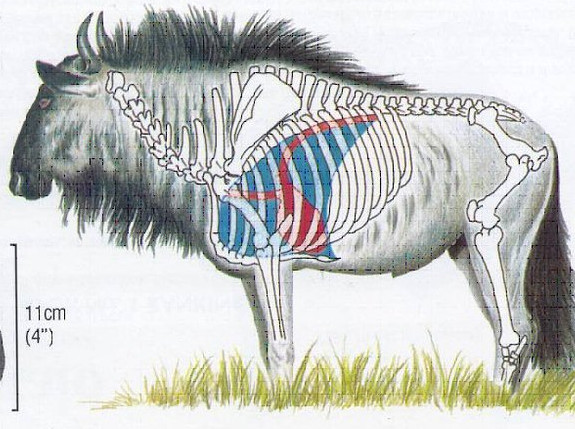
\includegraphics[width=0.2\textwidth]{../PCA/Skelettbilder_klein/Gnu.jpg}}~
\subfloat[Groenlandwal]{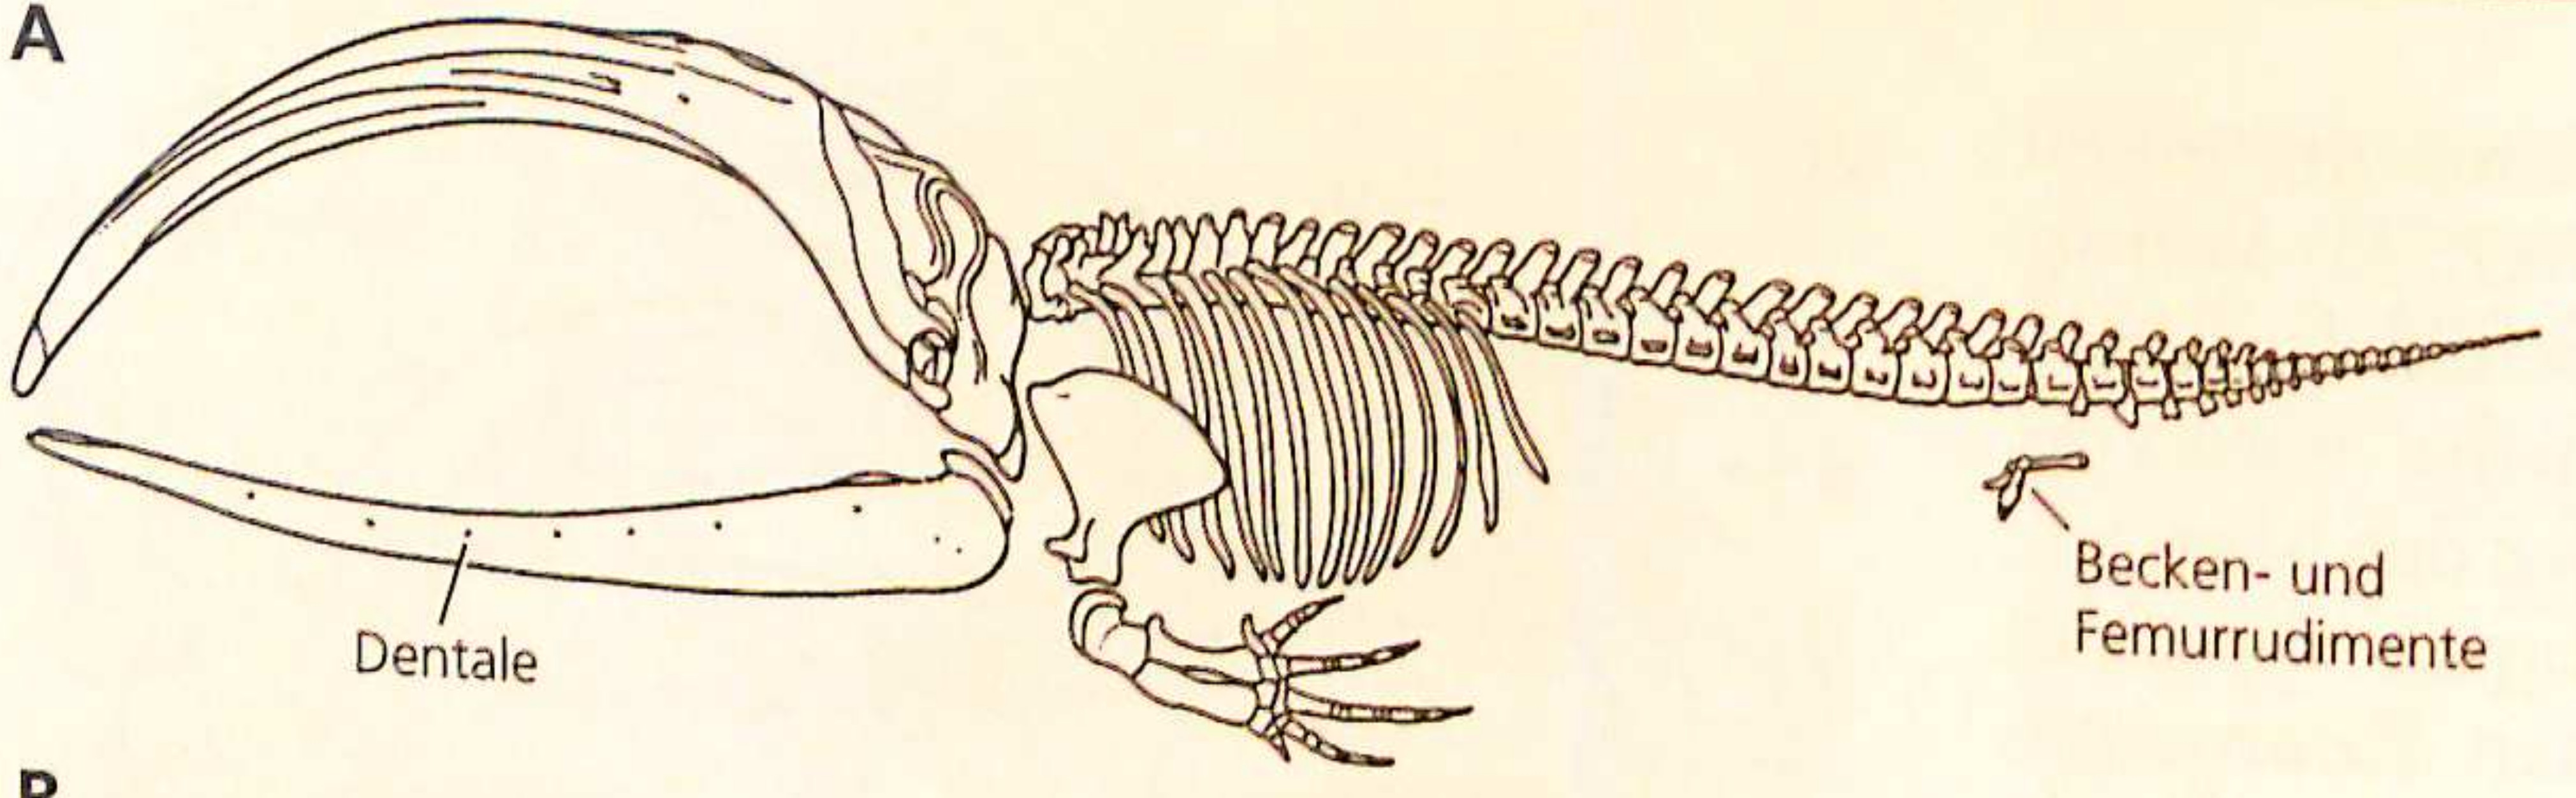
\includegraphics[width=0.2\textwidth]{../PCA/Skelettbilder_klein/Groenlandwal.jpg}}
\\
\subfloat[Ichthyornis]{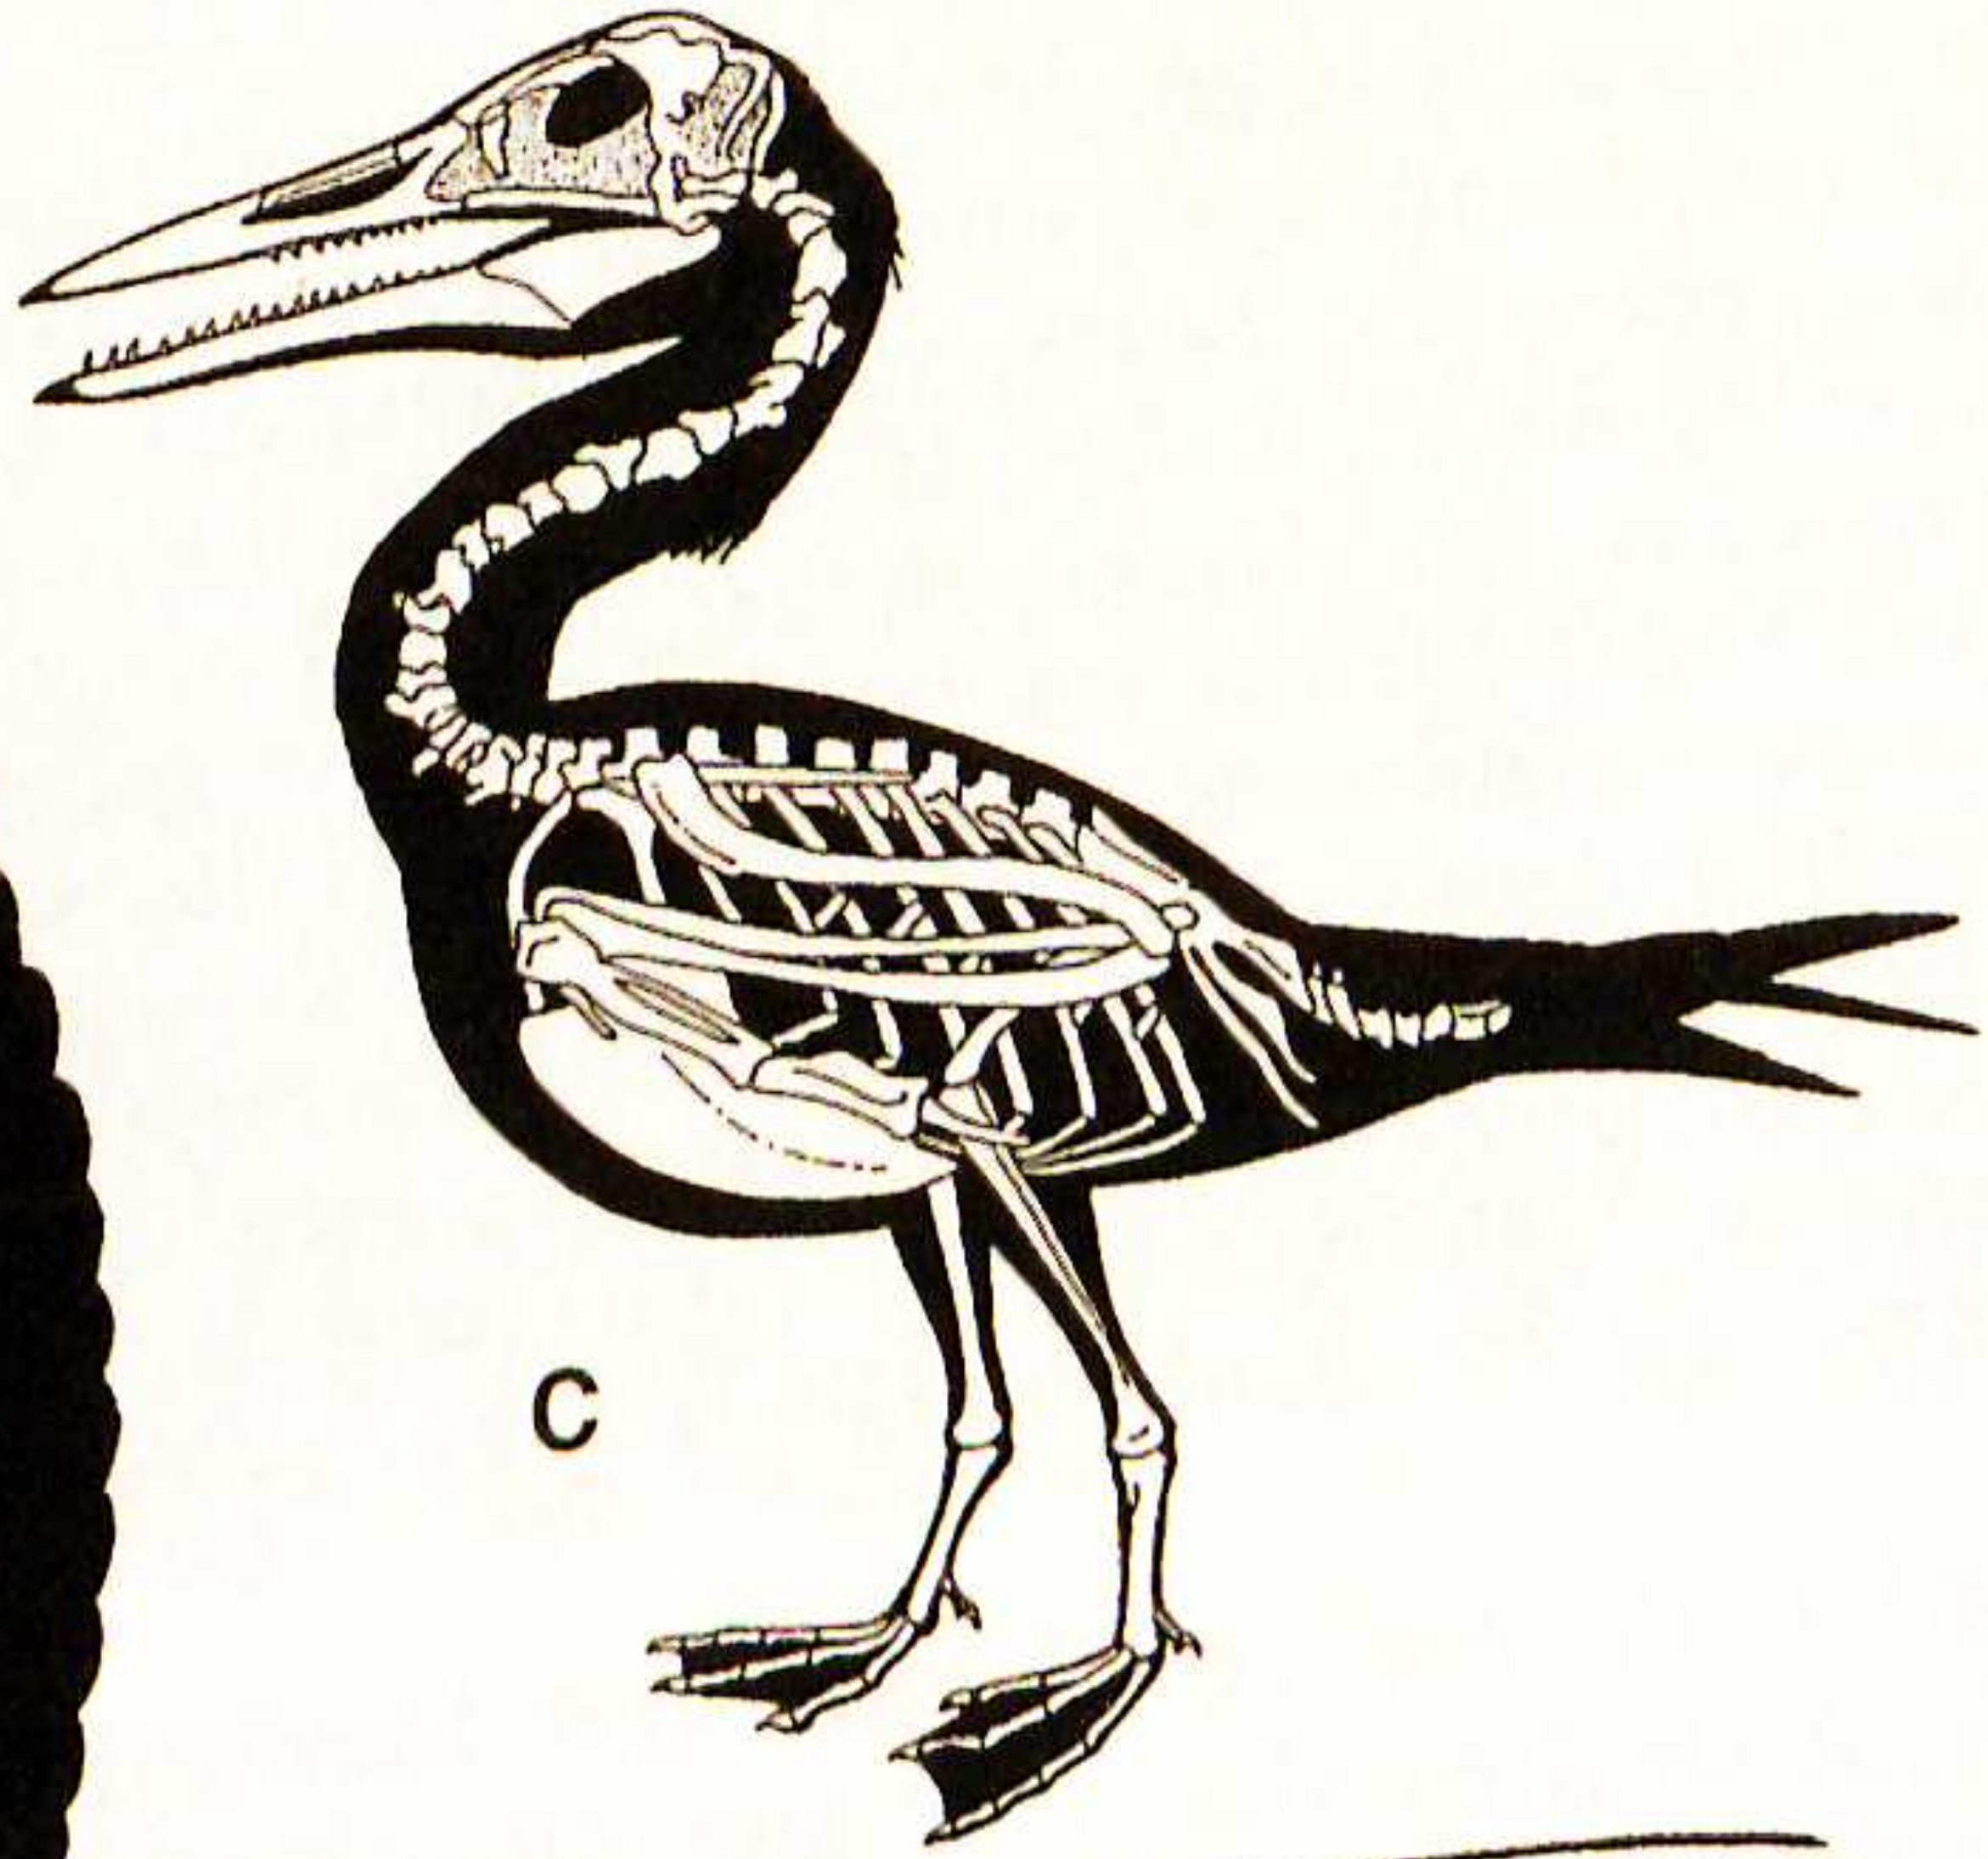
\includegraphics[width=0.2\textwidth]{../PCA/Skelettbilder_klein/Ichthyornis.jpg}}~
\subfloat[Ichthyosaurus]{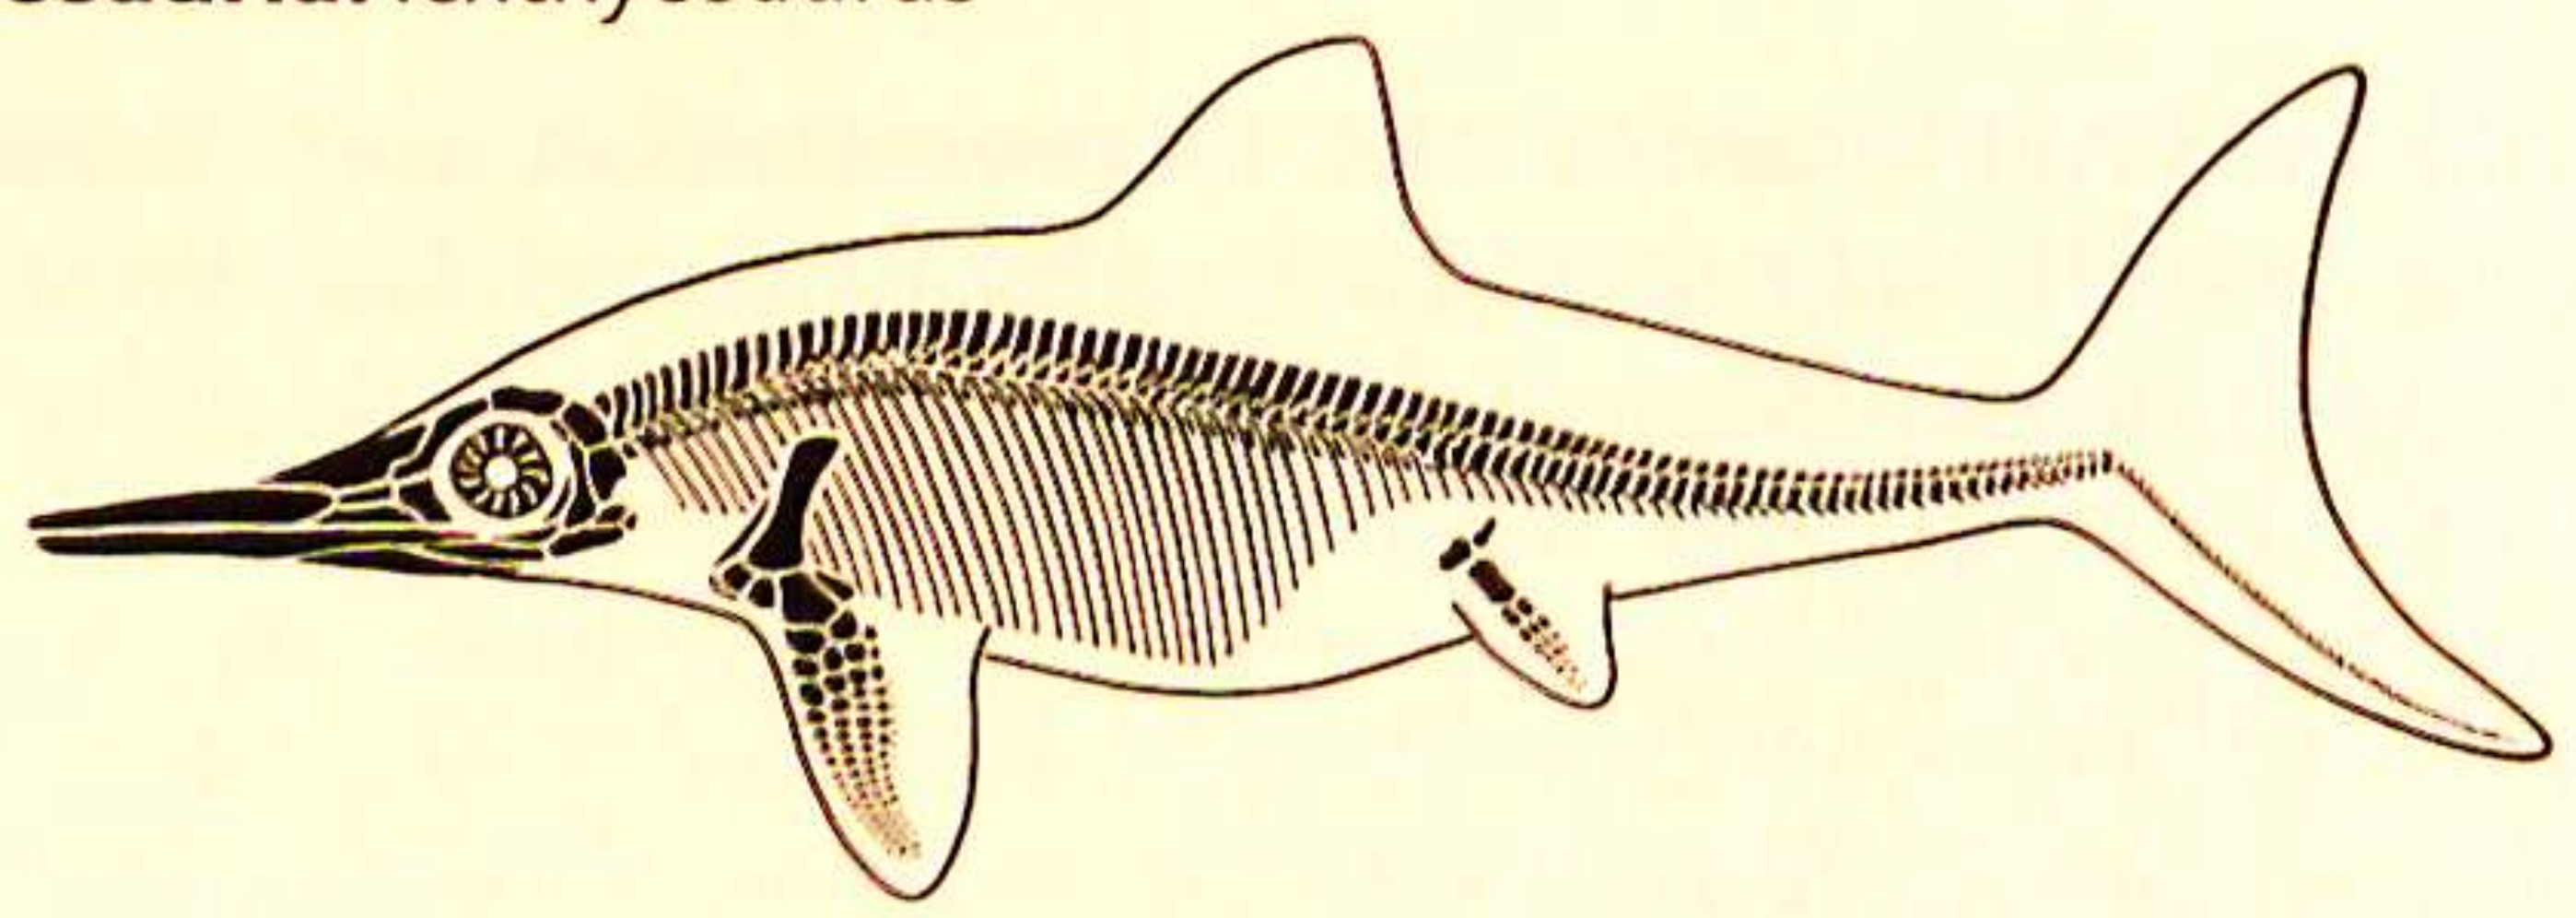
\includegraphics[width=0.2\textwidth]{../PCA/Skelettbilder_klein/Ichthyosaurus.jpg}}~
\subfloat[Ichthyostega]{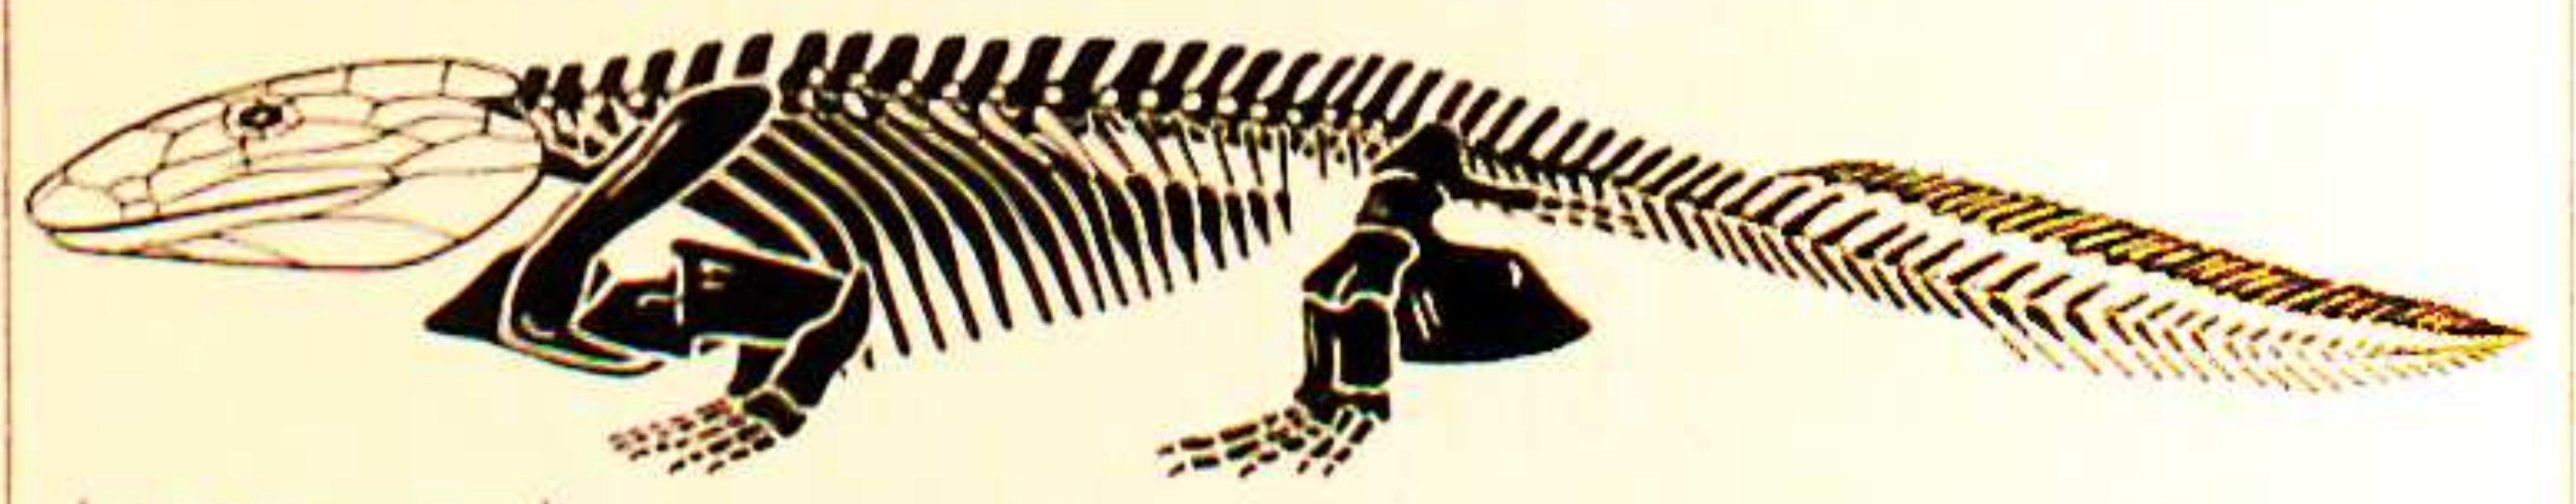
\includegraphics[width=0.2\textwidth]{../PCA/Skelettbilder_klein/Ichthyostega.jpg}}~
\subfloat[Kaenguru]{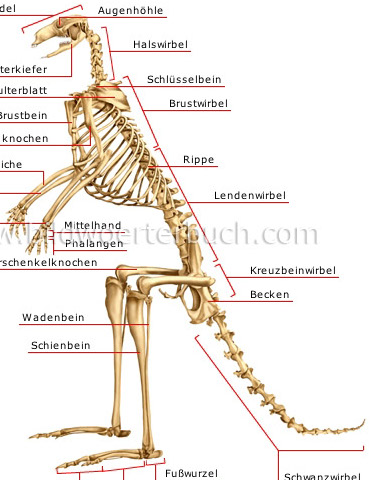
\includegraphics[width=0.2\textwidth]{../PCA/Skelettbilder_klein/Kaenguru.jpg}}~
\subfloat[Kaffernbueffel]{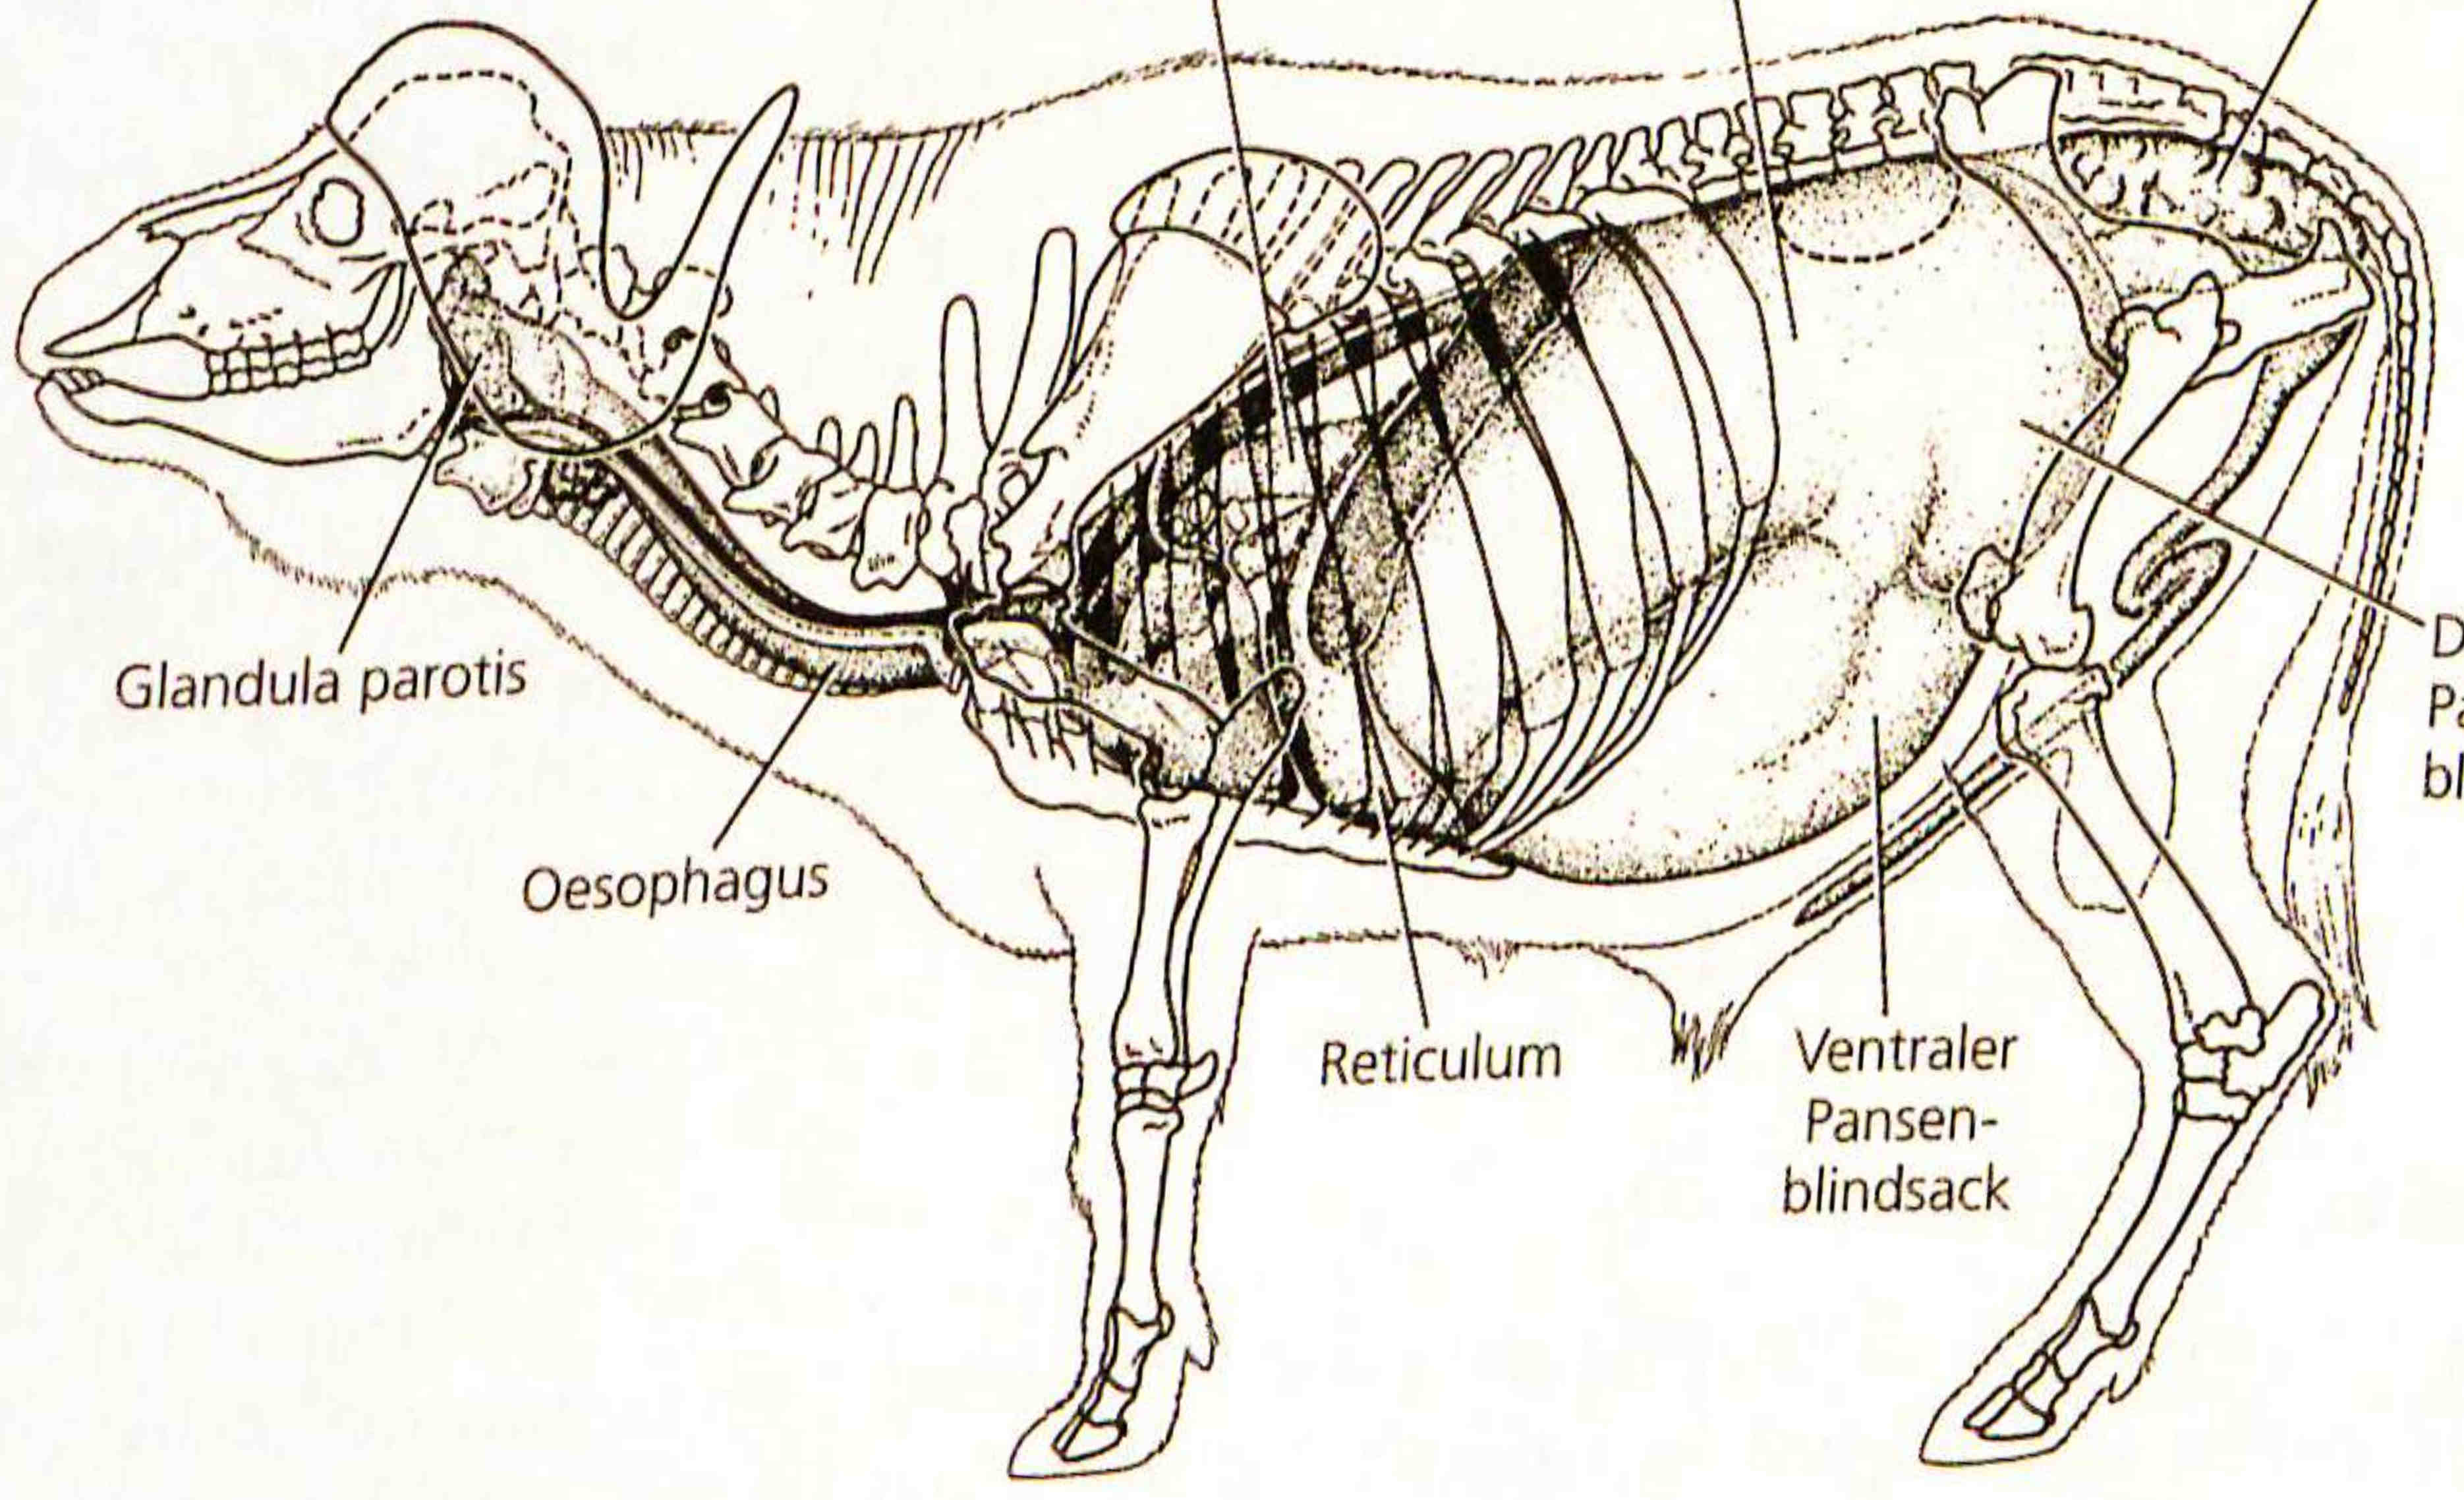
\includegraphics[width=0.2\textwidth]{../PCA/Skelettbilder_klein/Kaffernbueffel.jpg}}
\\
\subfloat[Kaninchen]{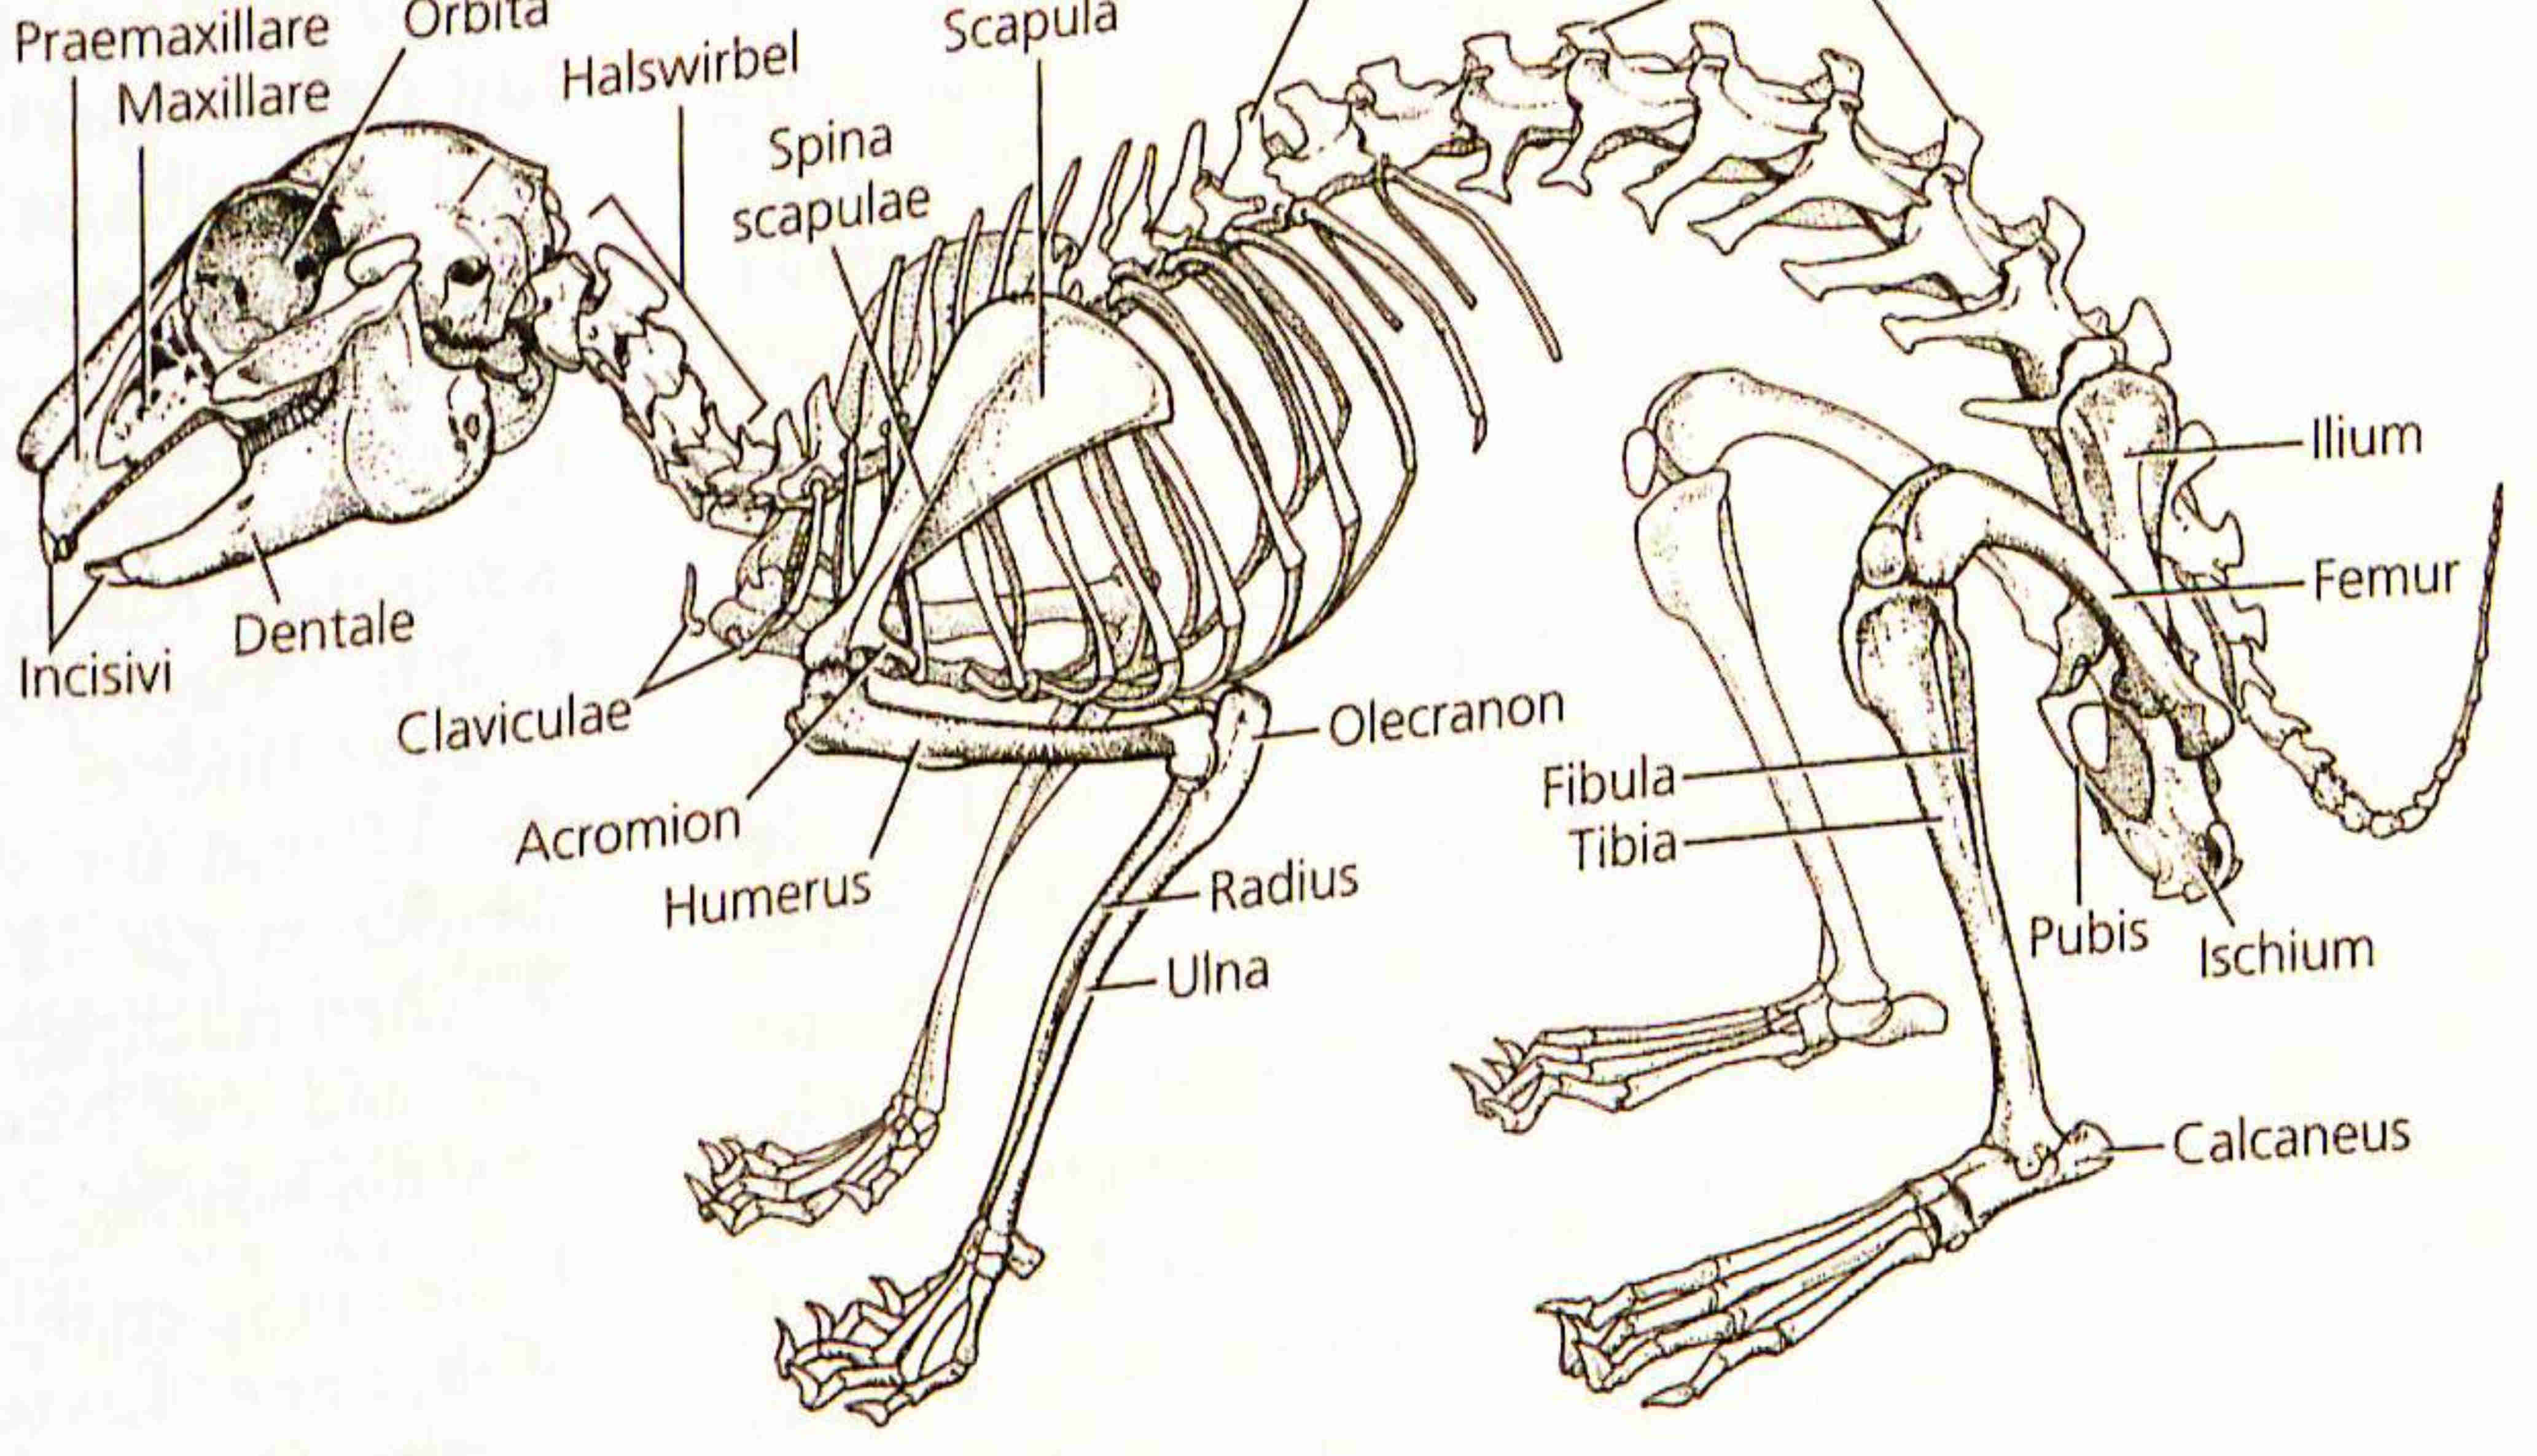
\includegraphics[width=0.2\textwidth]{../PCA/Skelettbilder_klein/Kaninchen.jpg}}~
\subfloat[Klippschliefer]{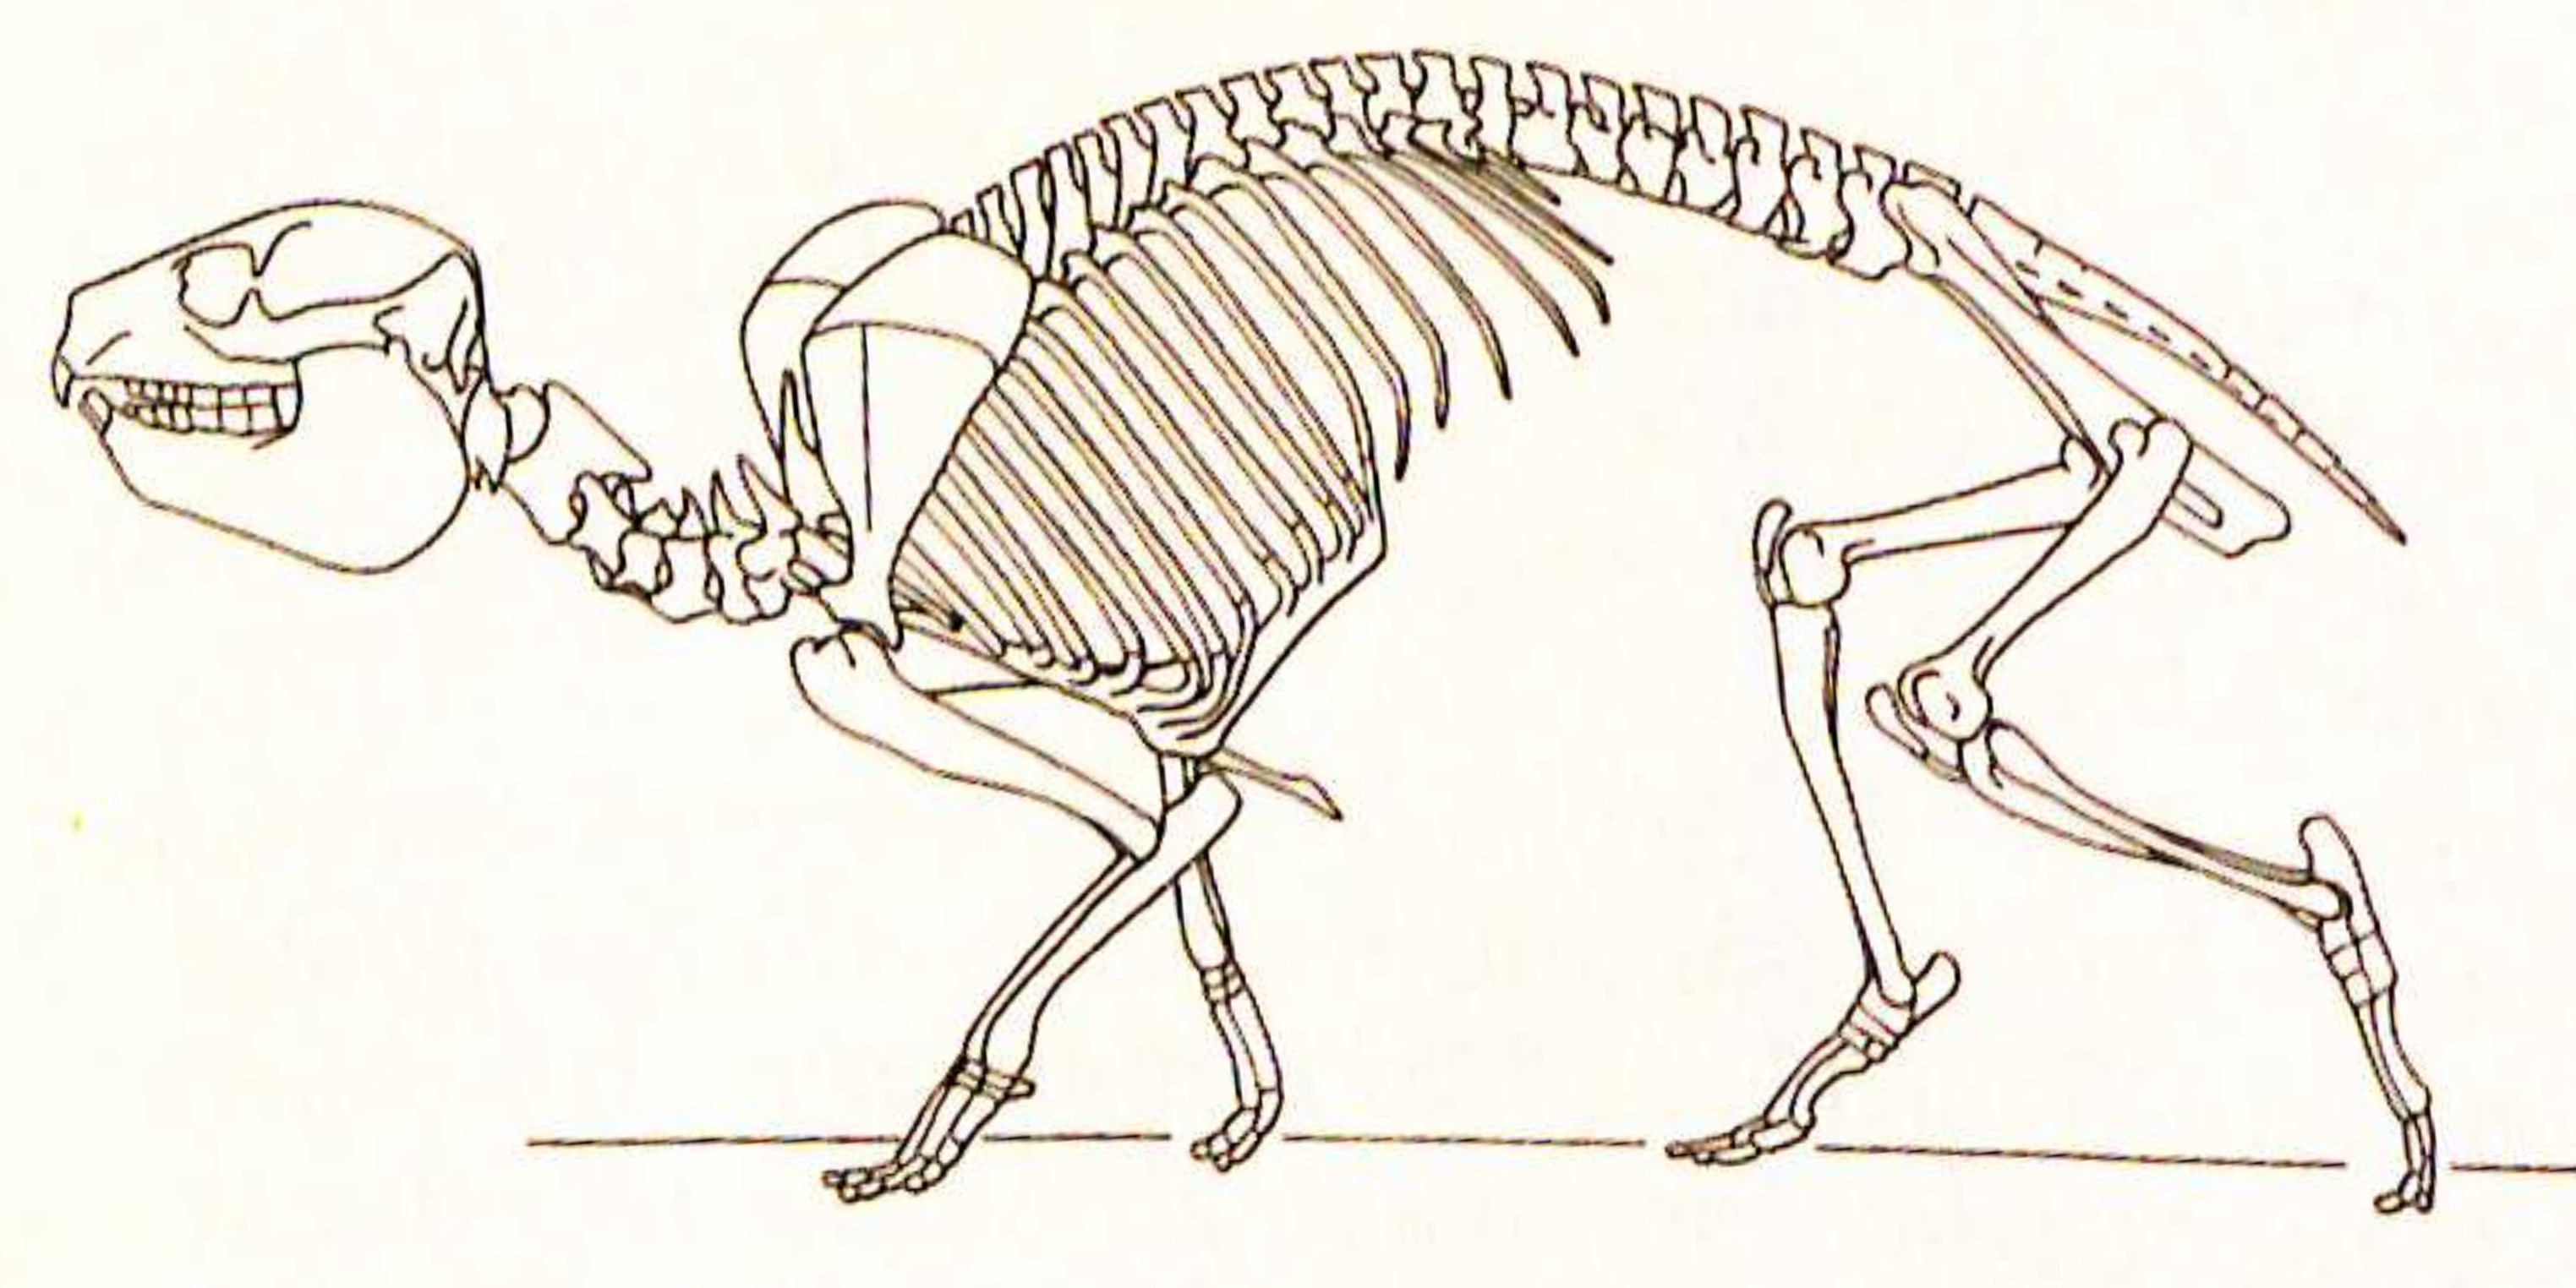
\includegraphics[width=0.2\textwidth]{../PCA/Skelettbilder_klein/Klippschliefer.jpg}}~
\subfloat[Koboldmaki]{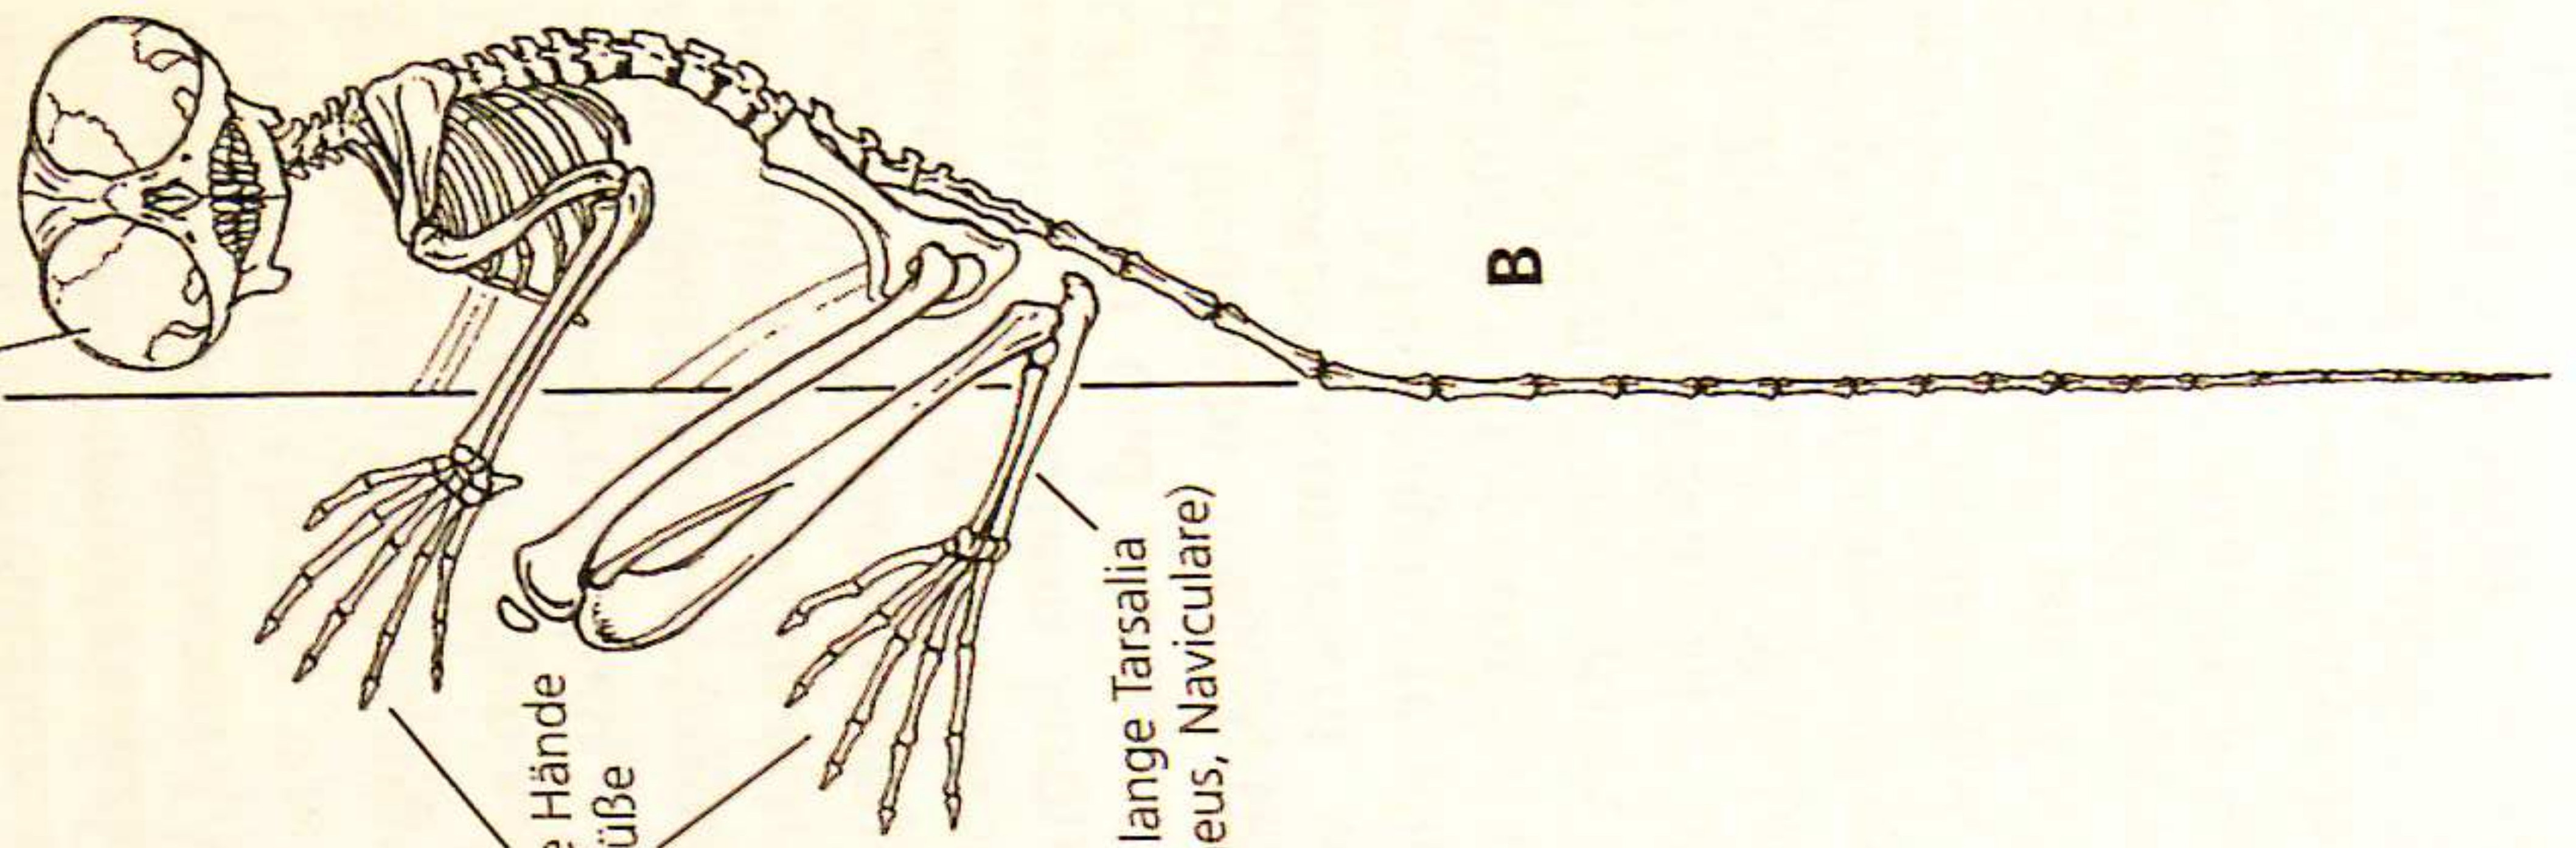
\includegraphics[width=0.2\textwidth]{../PCA/Skelettbilder_klein/Koboldmaki.jpg}}~
\subfloat[Krokodil]{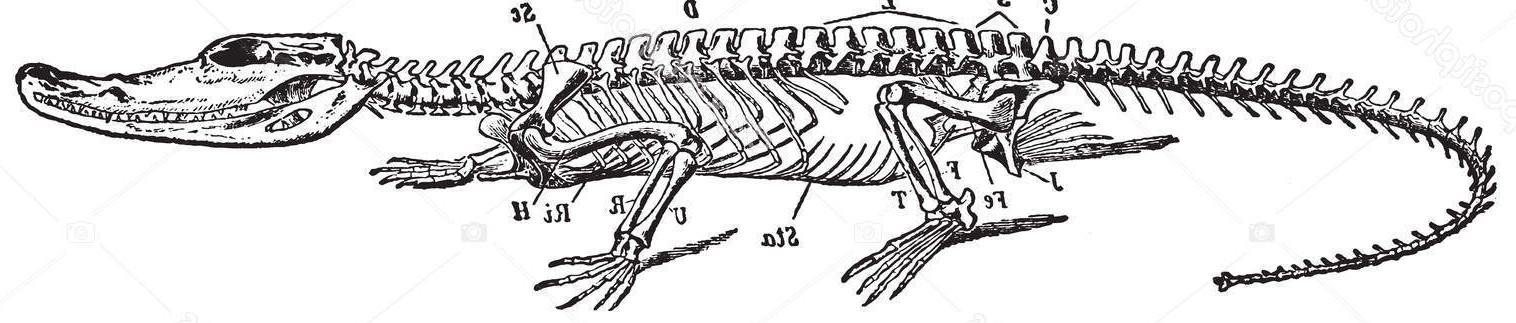
\includegraphics[width=0.2\textwidth]{../PCA/Skelettbilder_klein/Krokodil.jpg}}~
\subfloat[Landschildkroete]{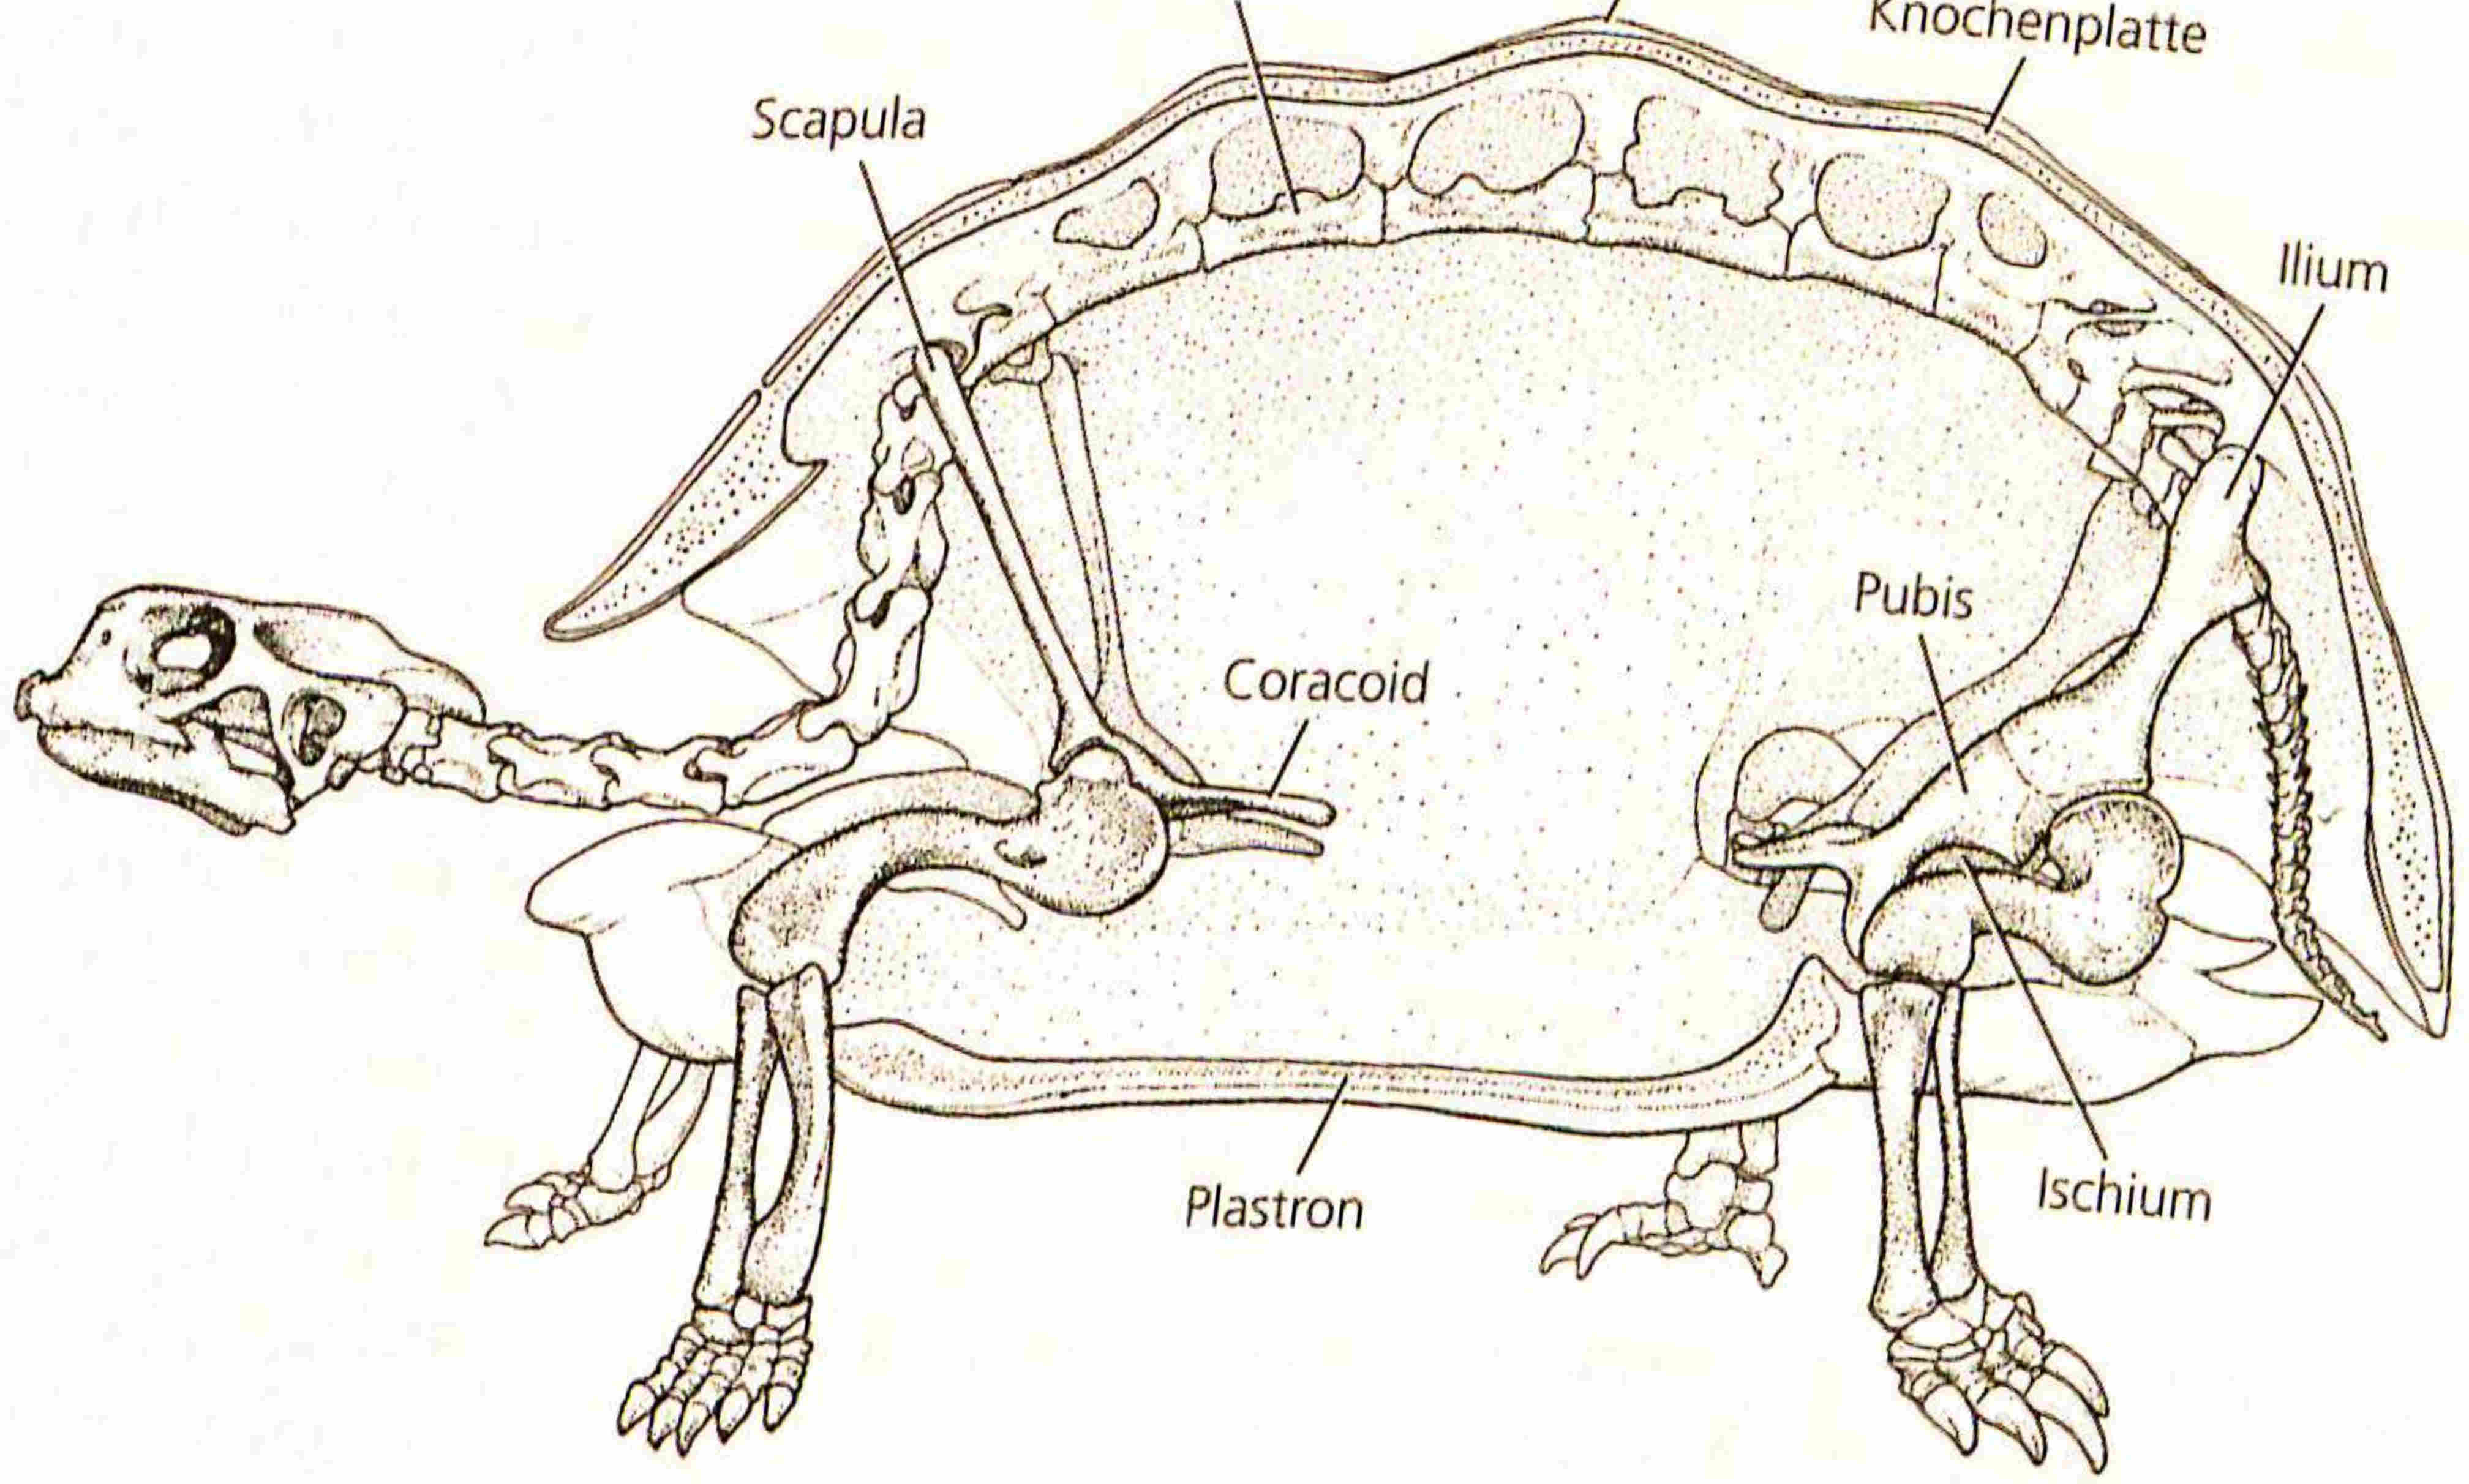
\includegraphics[width=0.2\textwidth]{../PCA/Skelettbilder_klein/Landschildkroete.jpg}}
\phantomcaption

\end{figure}
\begin{figure}
\ContinuedFloat

\subfloat[Ohrenrobbe]{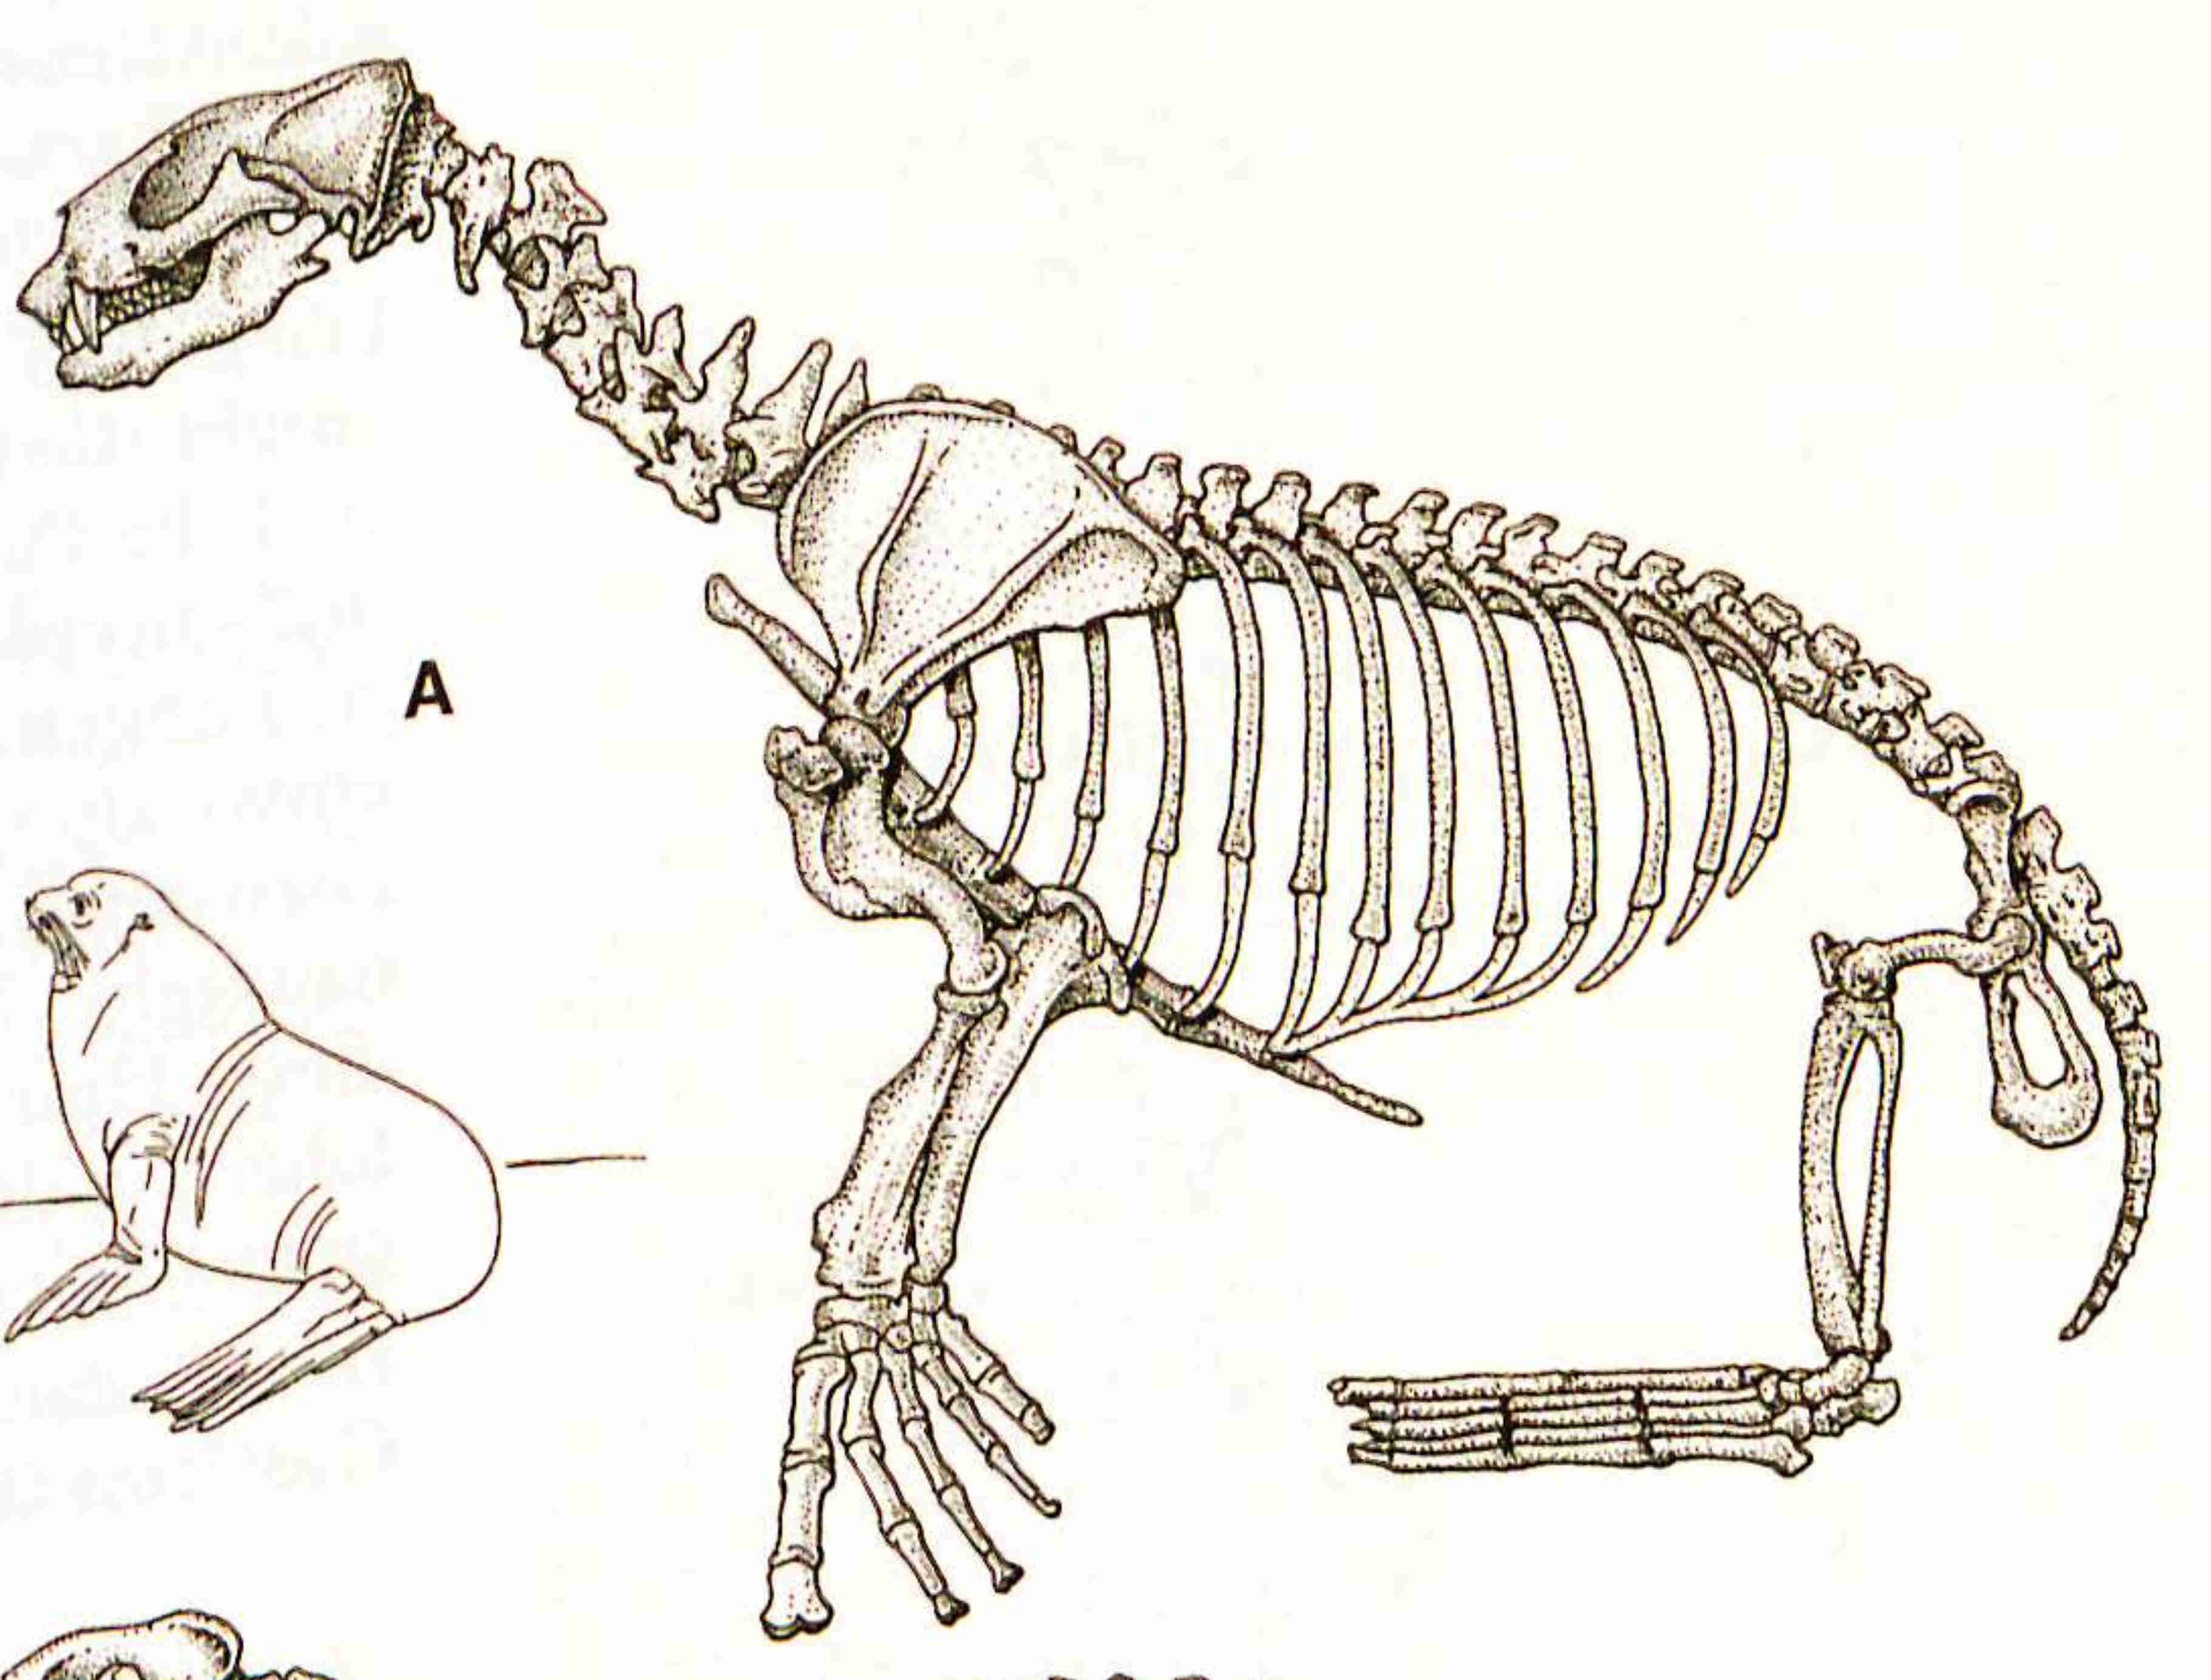
\includegraphics[width=0.2\textwidth]{../PCA/Skelettbilder_klein/Ohrenrobbe.jpg}}~
\subfloat[Panzerspitzmaus]{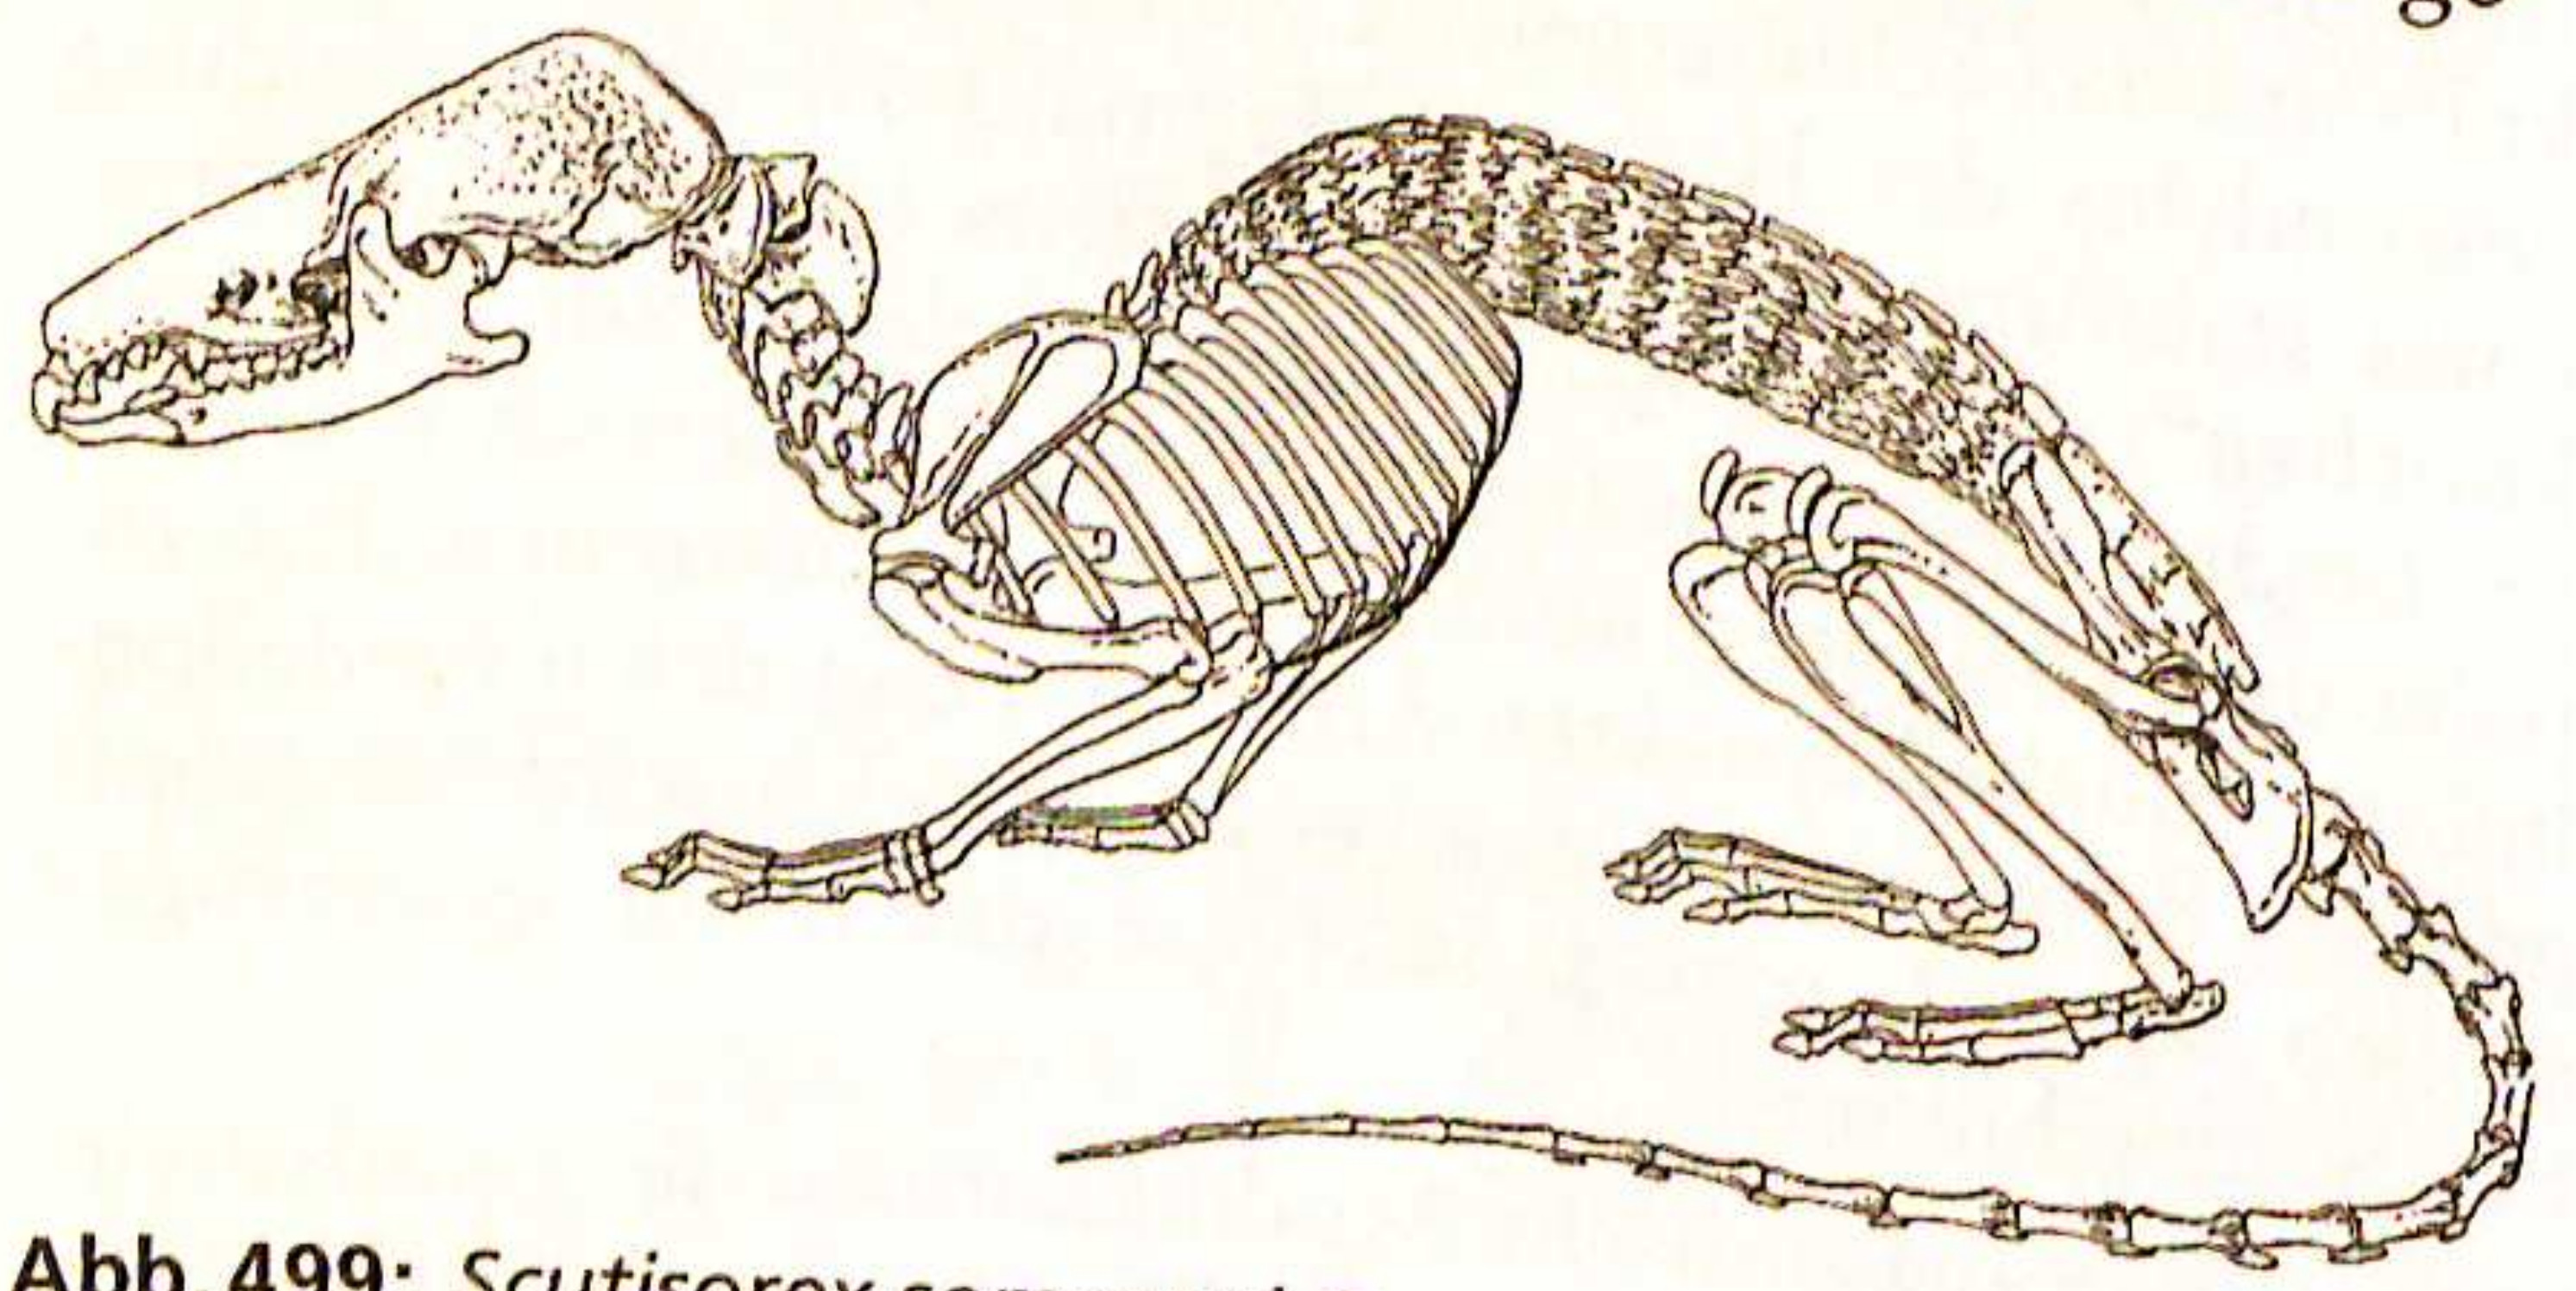
\includegraphics[width=0.2\textwidth]{../PCA/Skelettbilder_klein/Panzerspitzmaus.jpg}}~
\subfloat[Parasaurolophus walkeri]{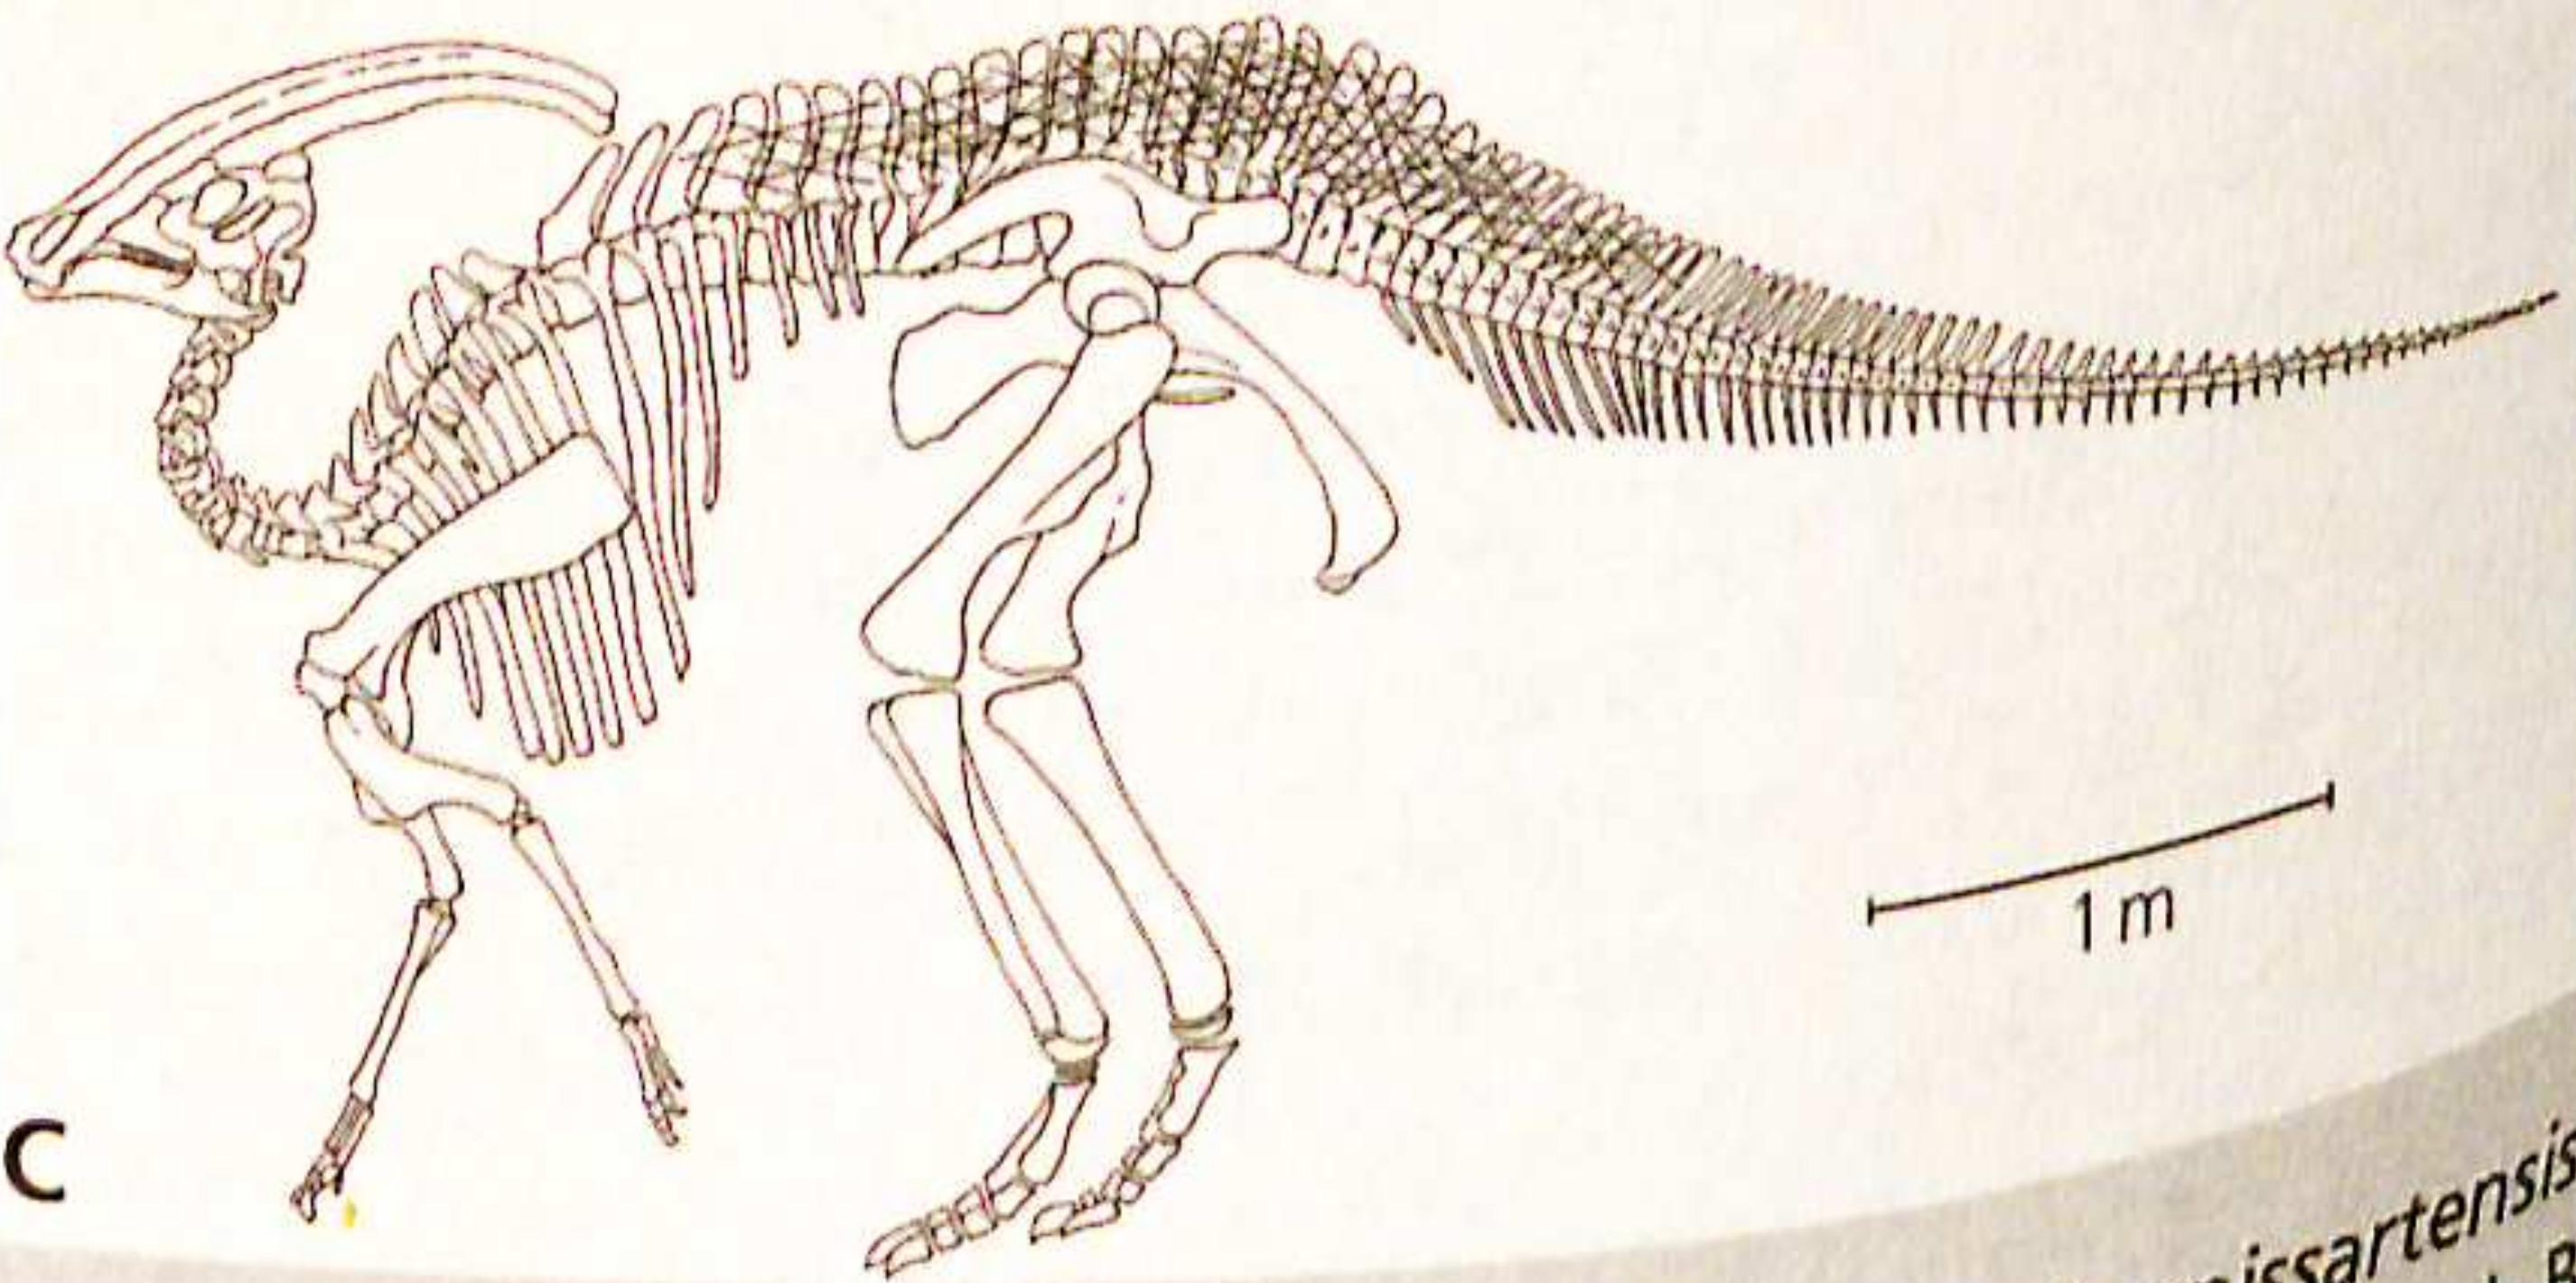
\includegraphics[width=0.2\textwidth]{../PCA/Skelettbilder_klein/Parasaurolophus_walkeri.jpg}}~
\subfloat[Peloneustes philarchus]{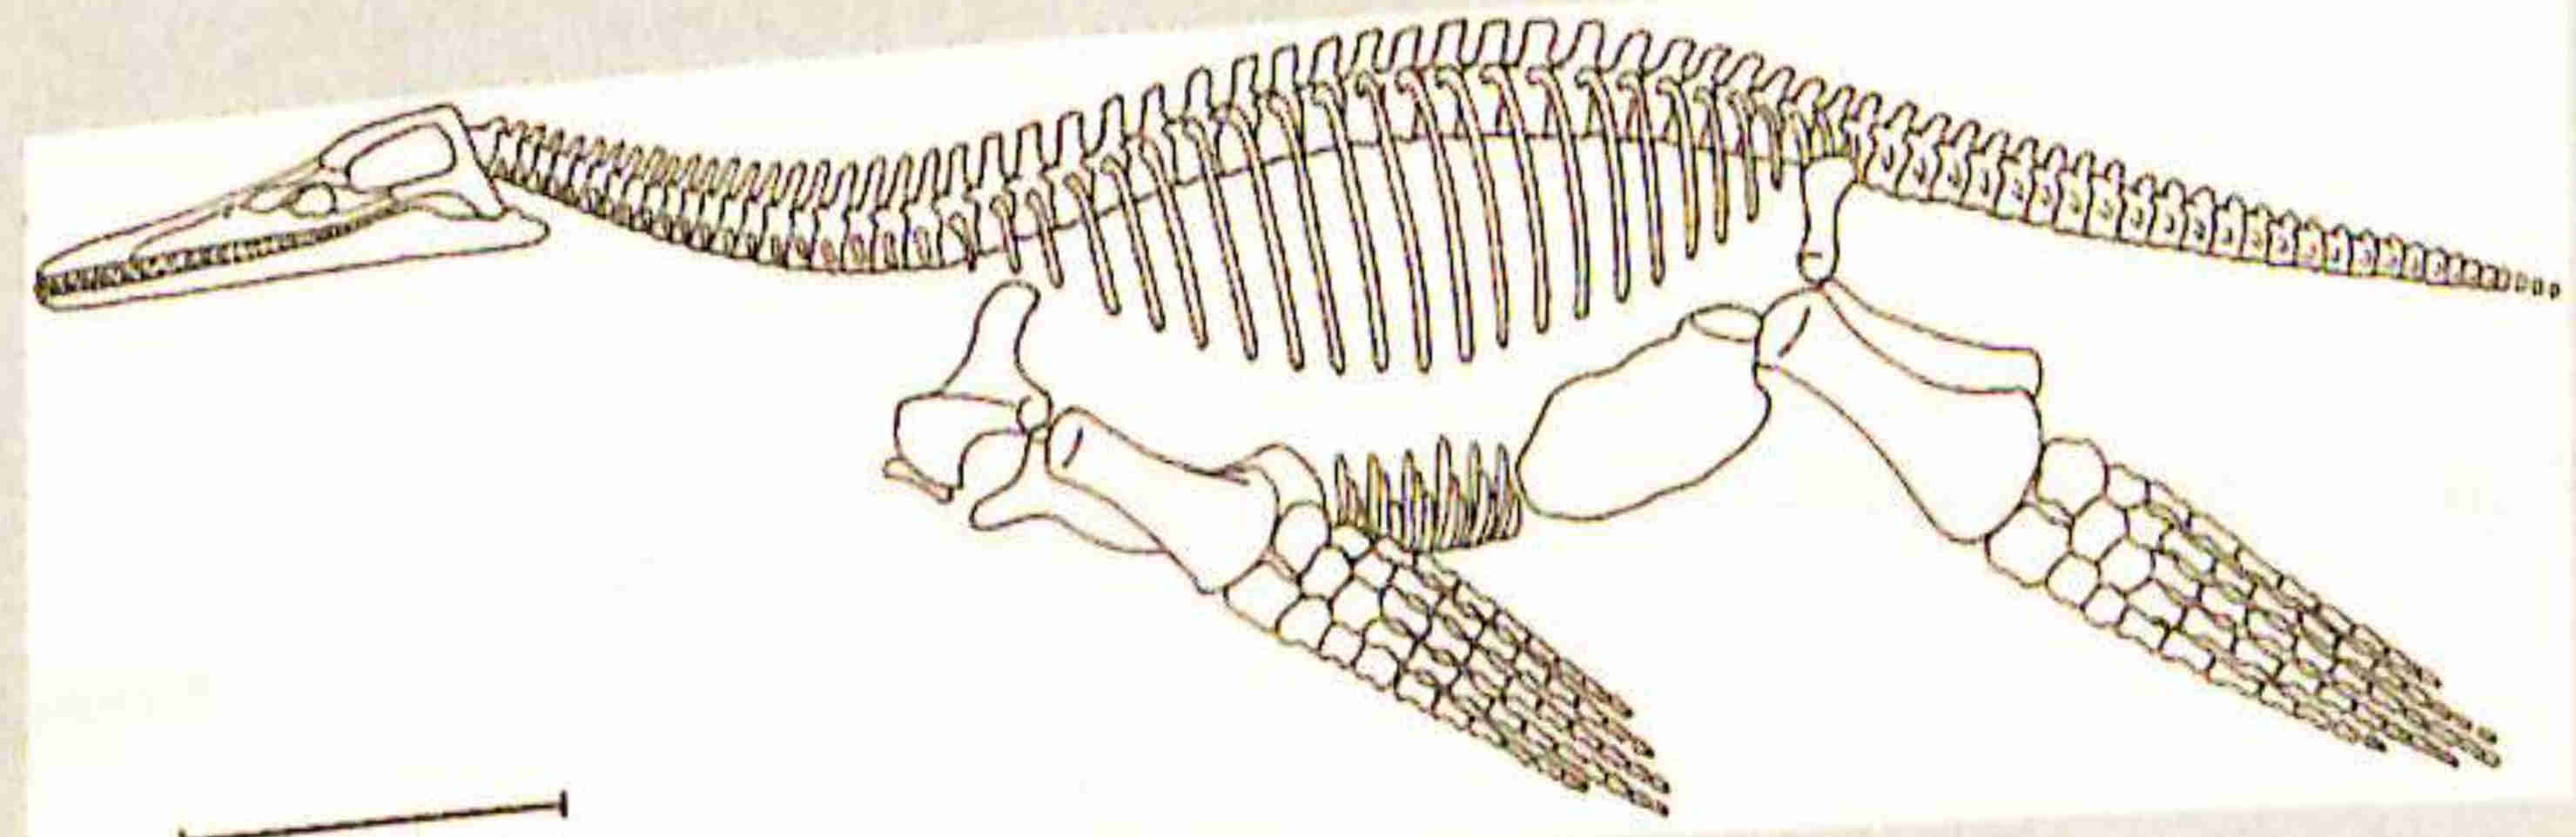
\includegraphics[width=0.2\textwidth]{../PCA/Skelettbilder_klein/Peloneustes_philarchus.jpg}}~
\subfloat[Pferd]{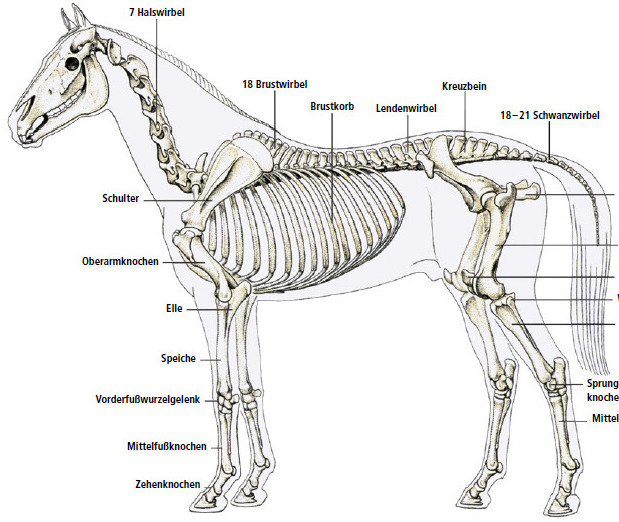
\includegraphics[width=0.2\textwidth]{../PCA/Skelettbilder_klein/Pferd.jpg}}
\\
\subfloat[Pottwal]{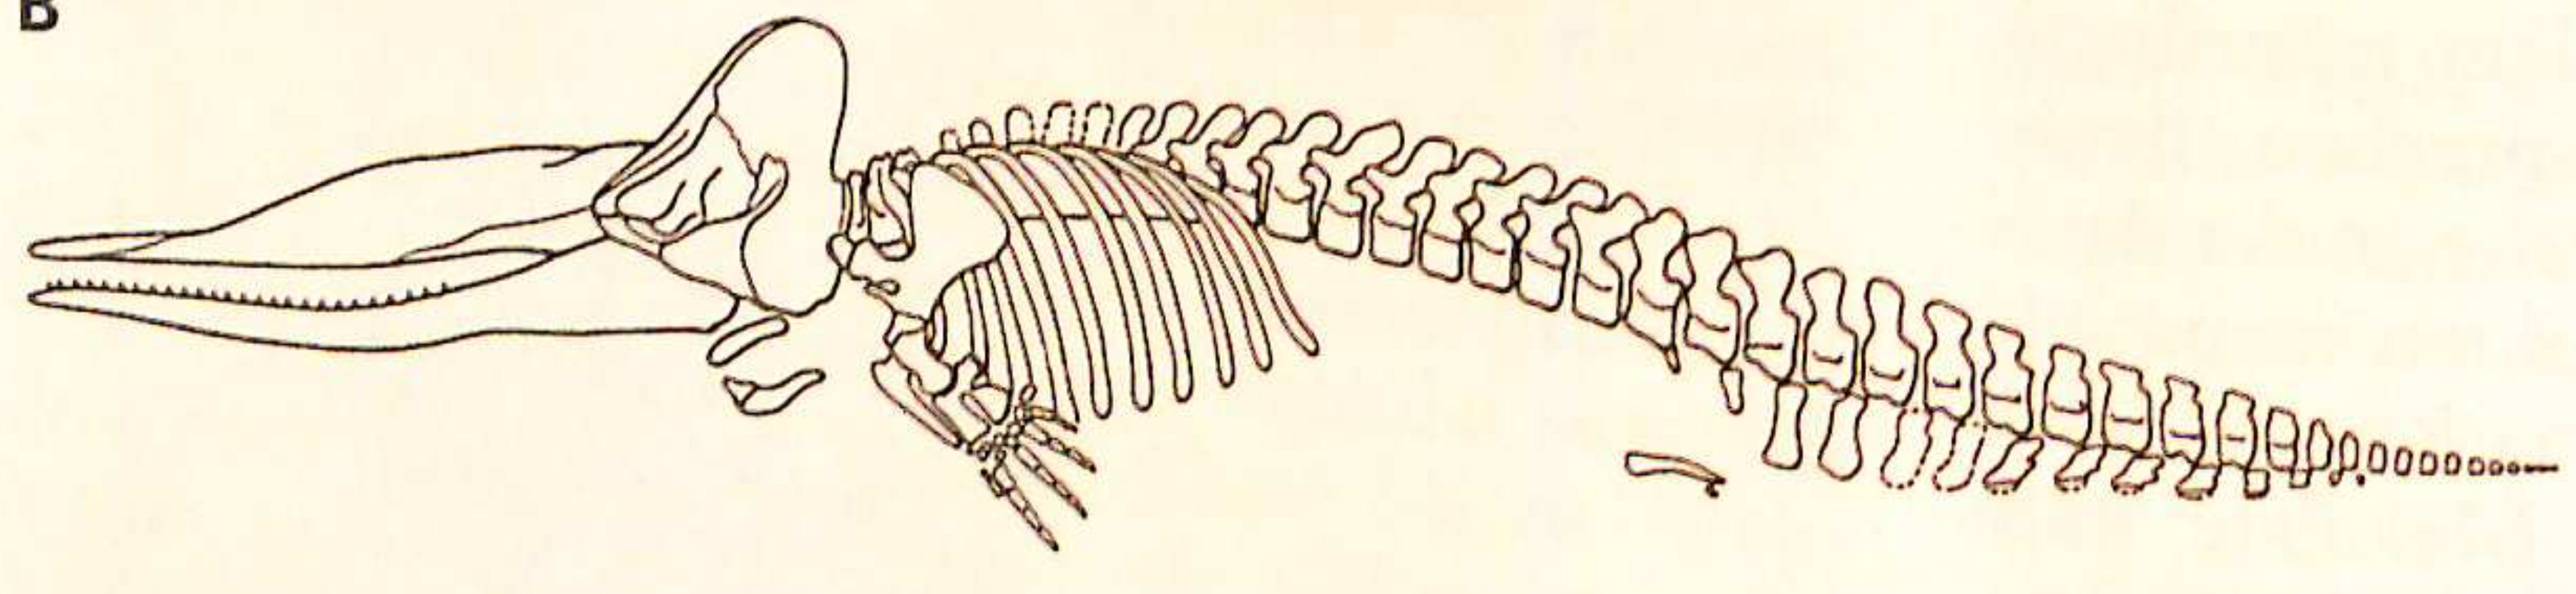
\includegraphics[width=0.2\textwidth]{../PCA/Skelettbilder_klein/Pottwal.jpg}}~
\subfloat[Rothirsch]{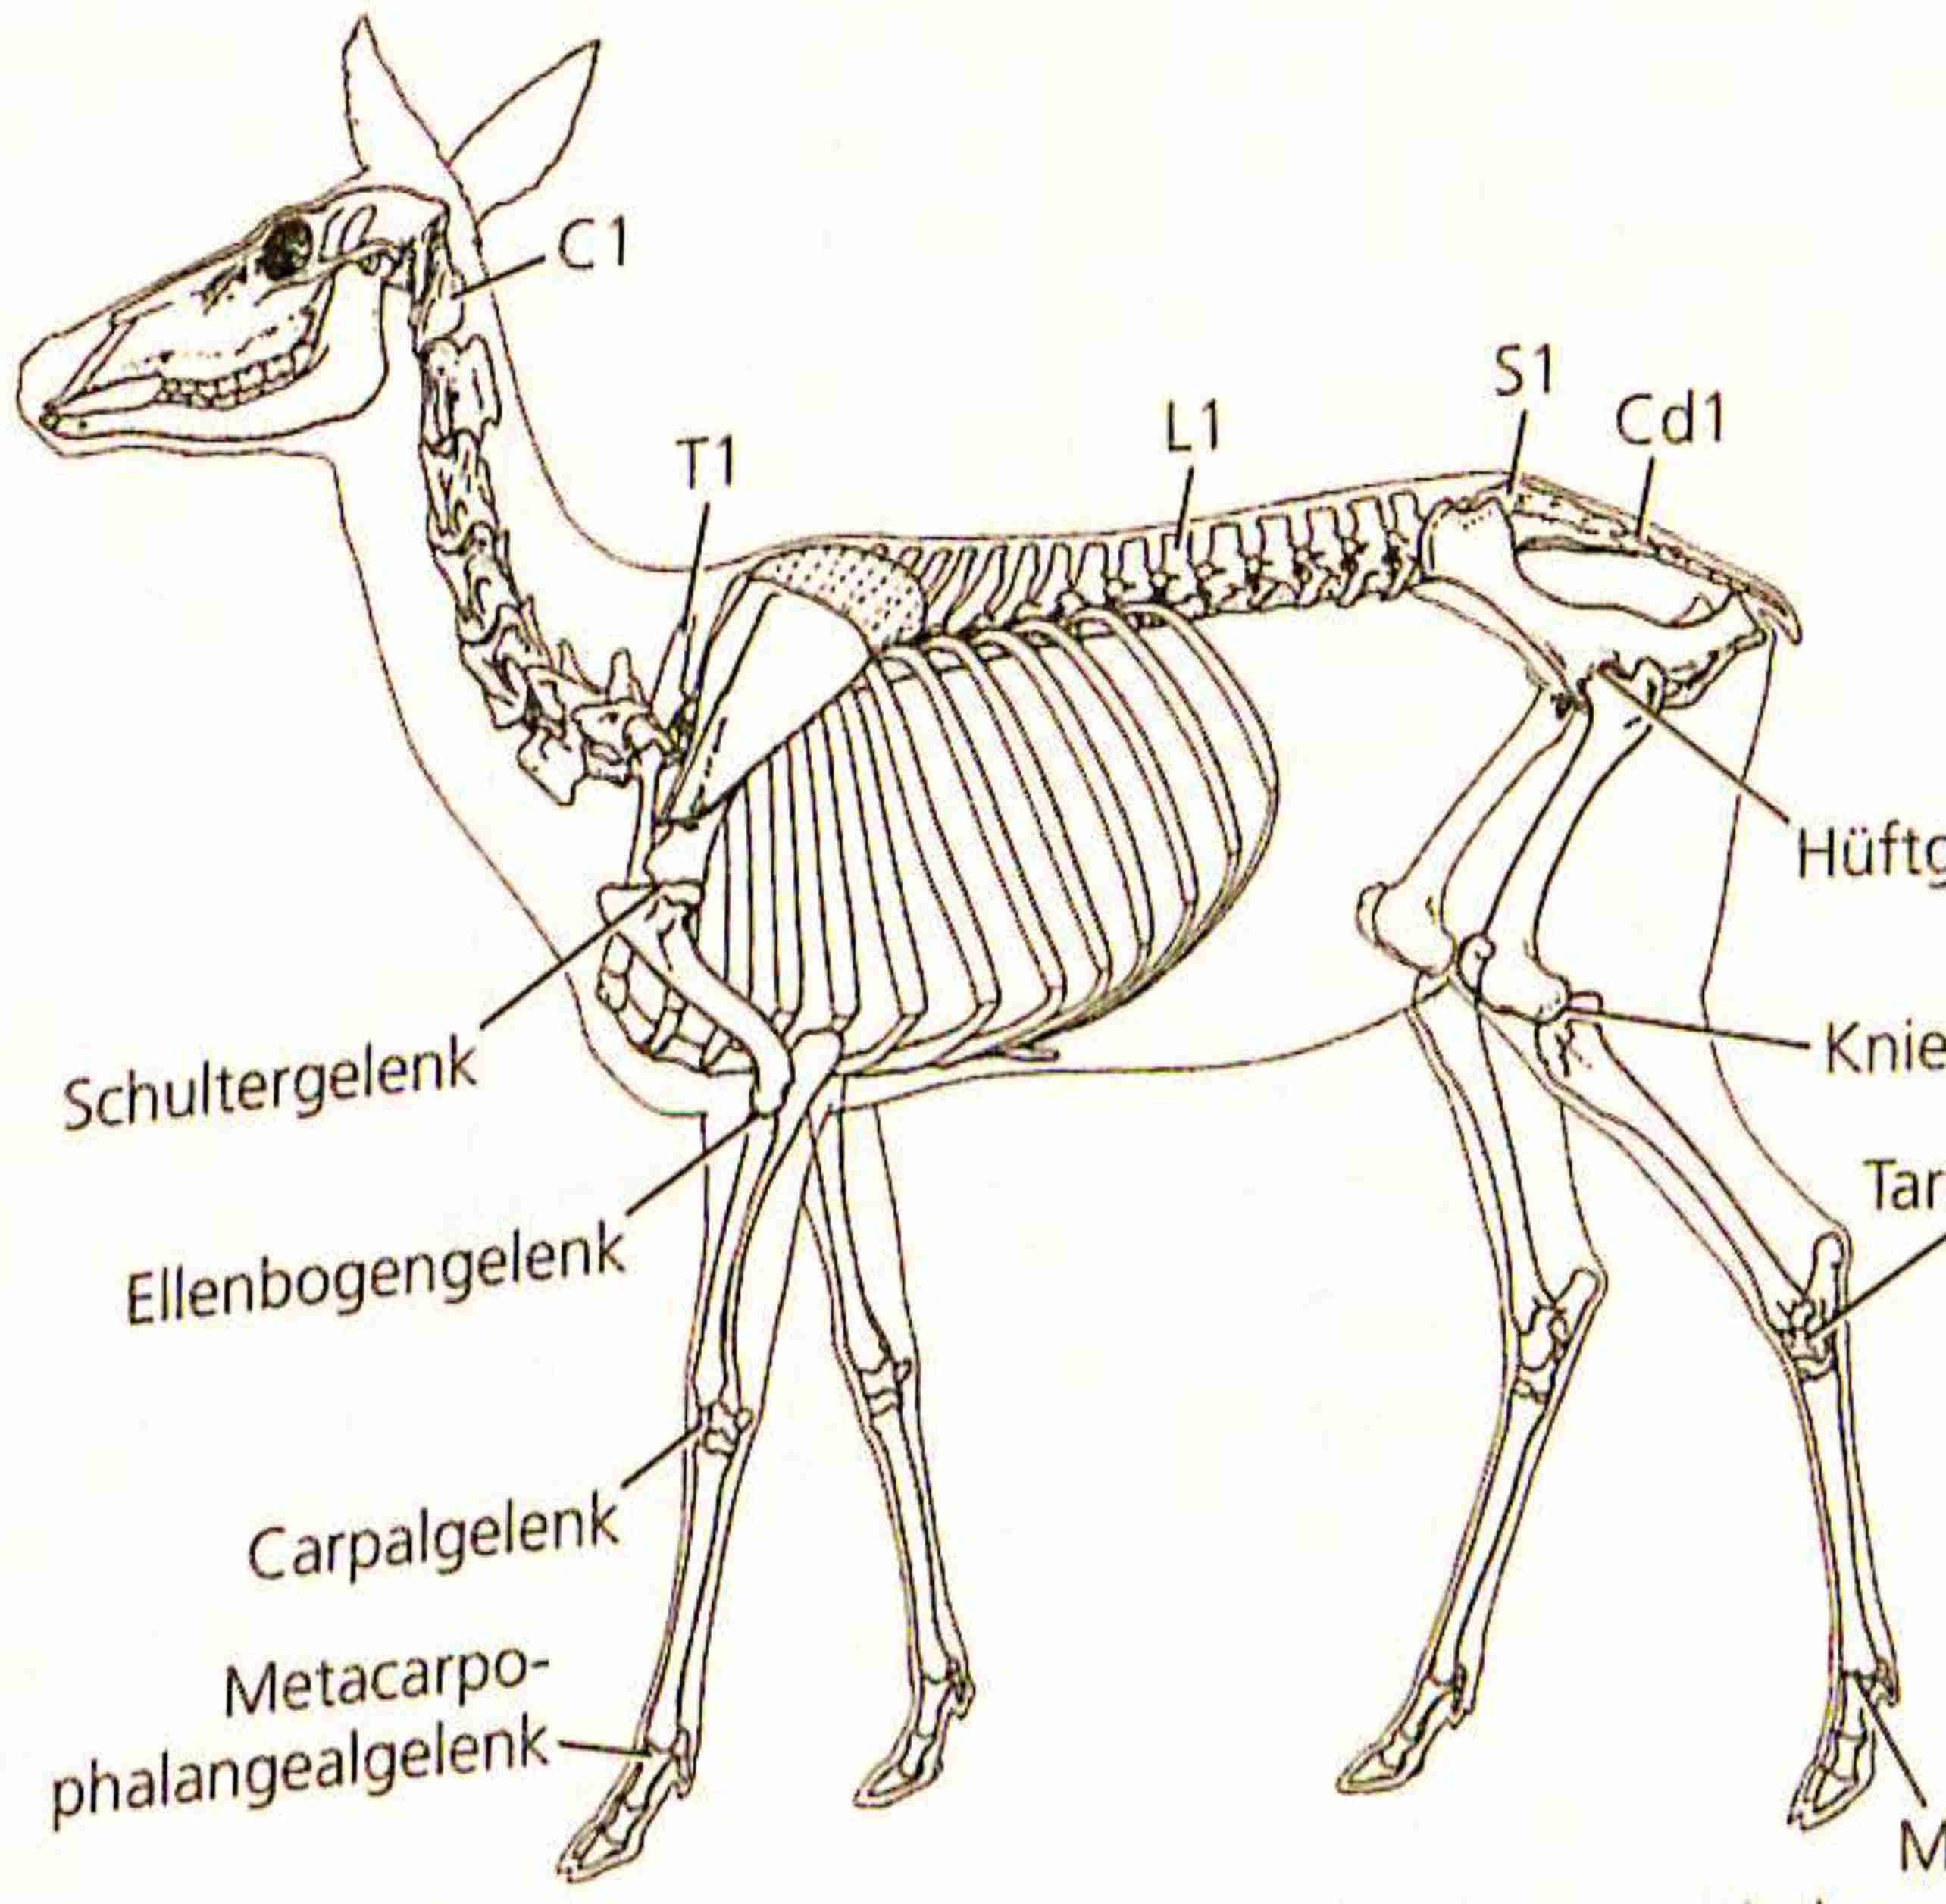
\includegraphics[width=0.2\textwidth]{../PCA/Skelettbilder_klein/Rothirsch.jpg}}~
\subfloat[Schwan]{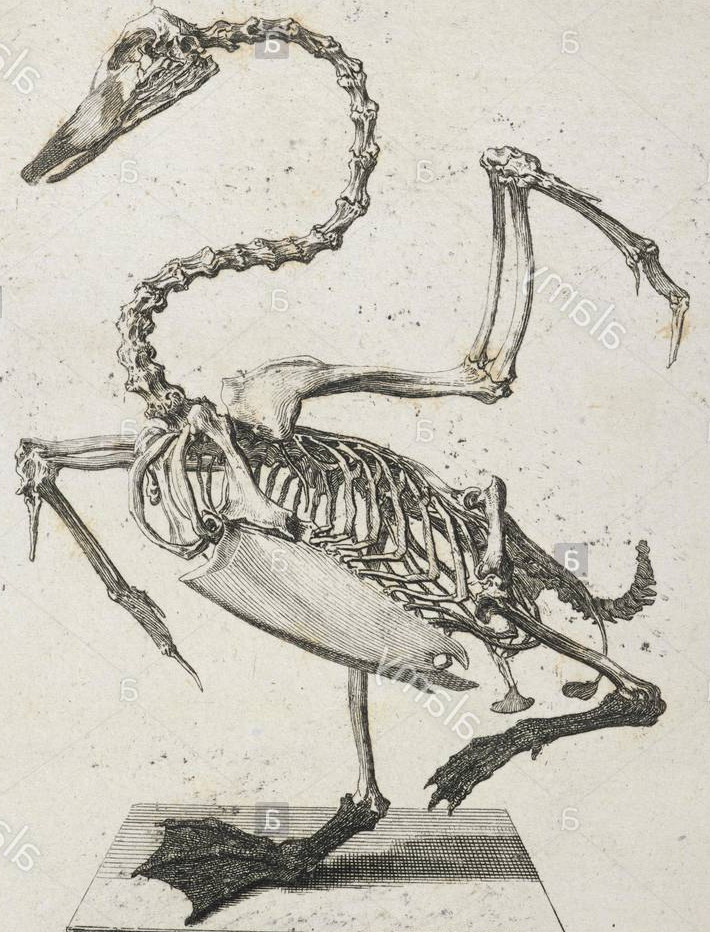
\includegraphics[width=0.2\textwidth]{../PCA/Skelettbilder_klein/Schwan.jpg}}~
\subfloat[Schwein]{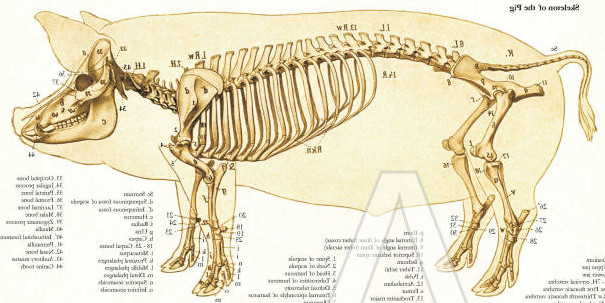
\includegraphics[width=0.2\textwidth]{../PCA/Skelettbilder_klein/Schwein.jpg}}~
\subfloat[Seehund]{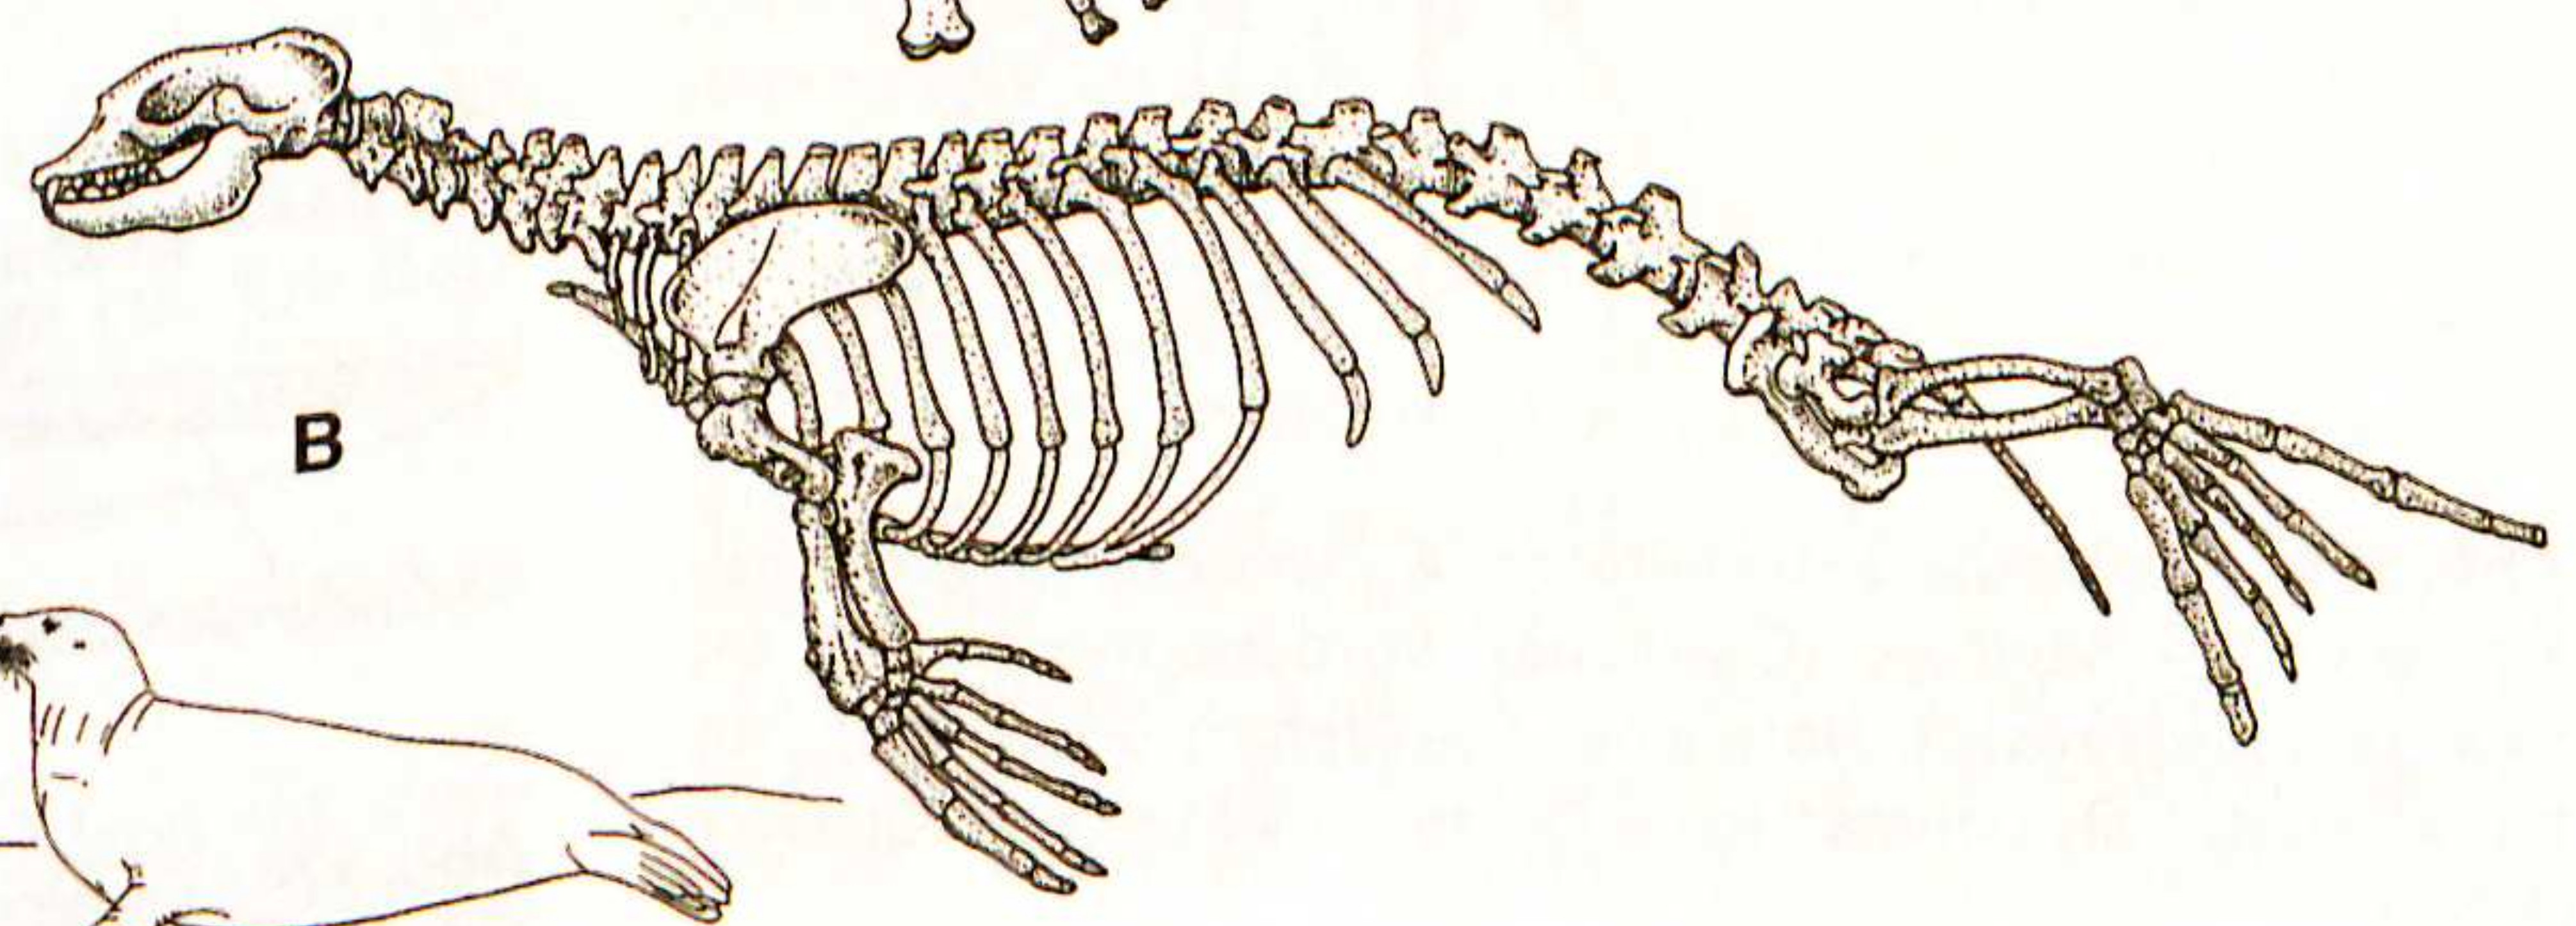
\includegraphics[width=0.2\textwidth]{../PCA/Skelettbilder_klein/Seehund.jpg}}
\\
\subfloat[Sinornis]{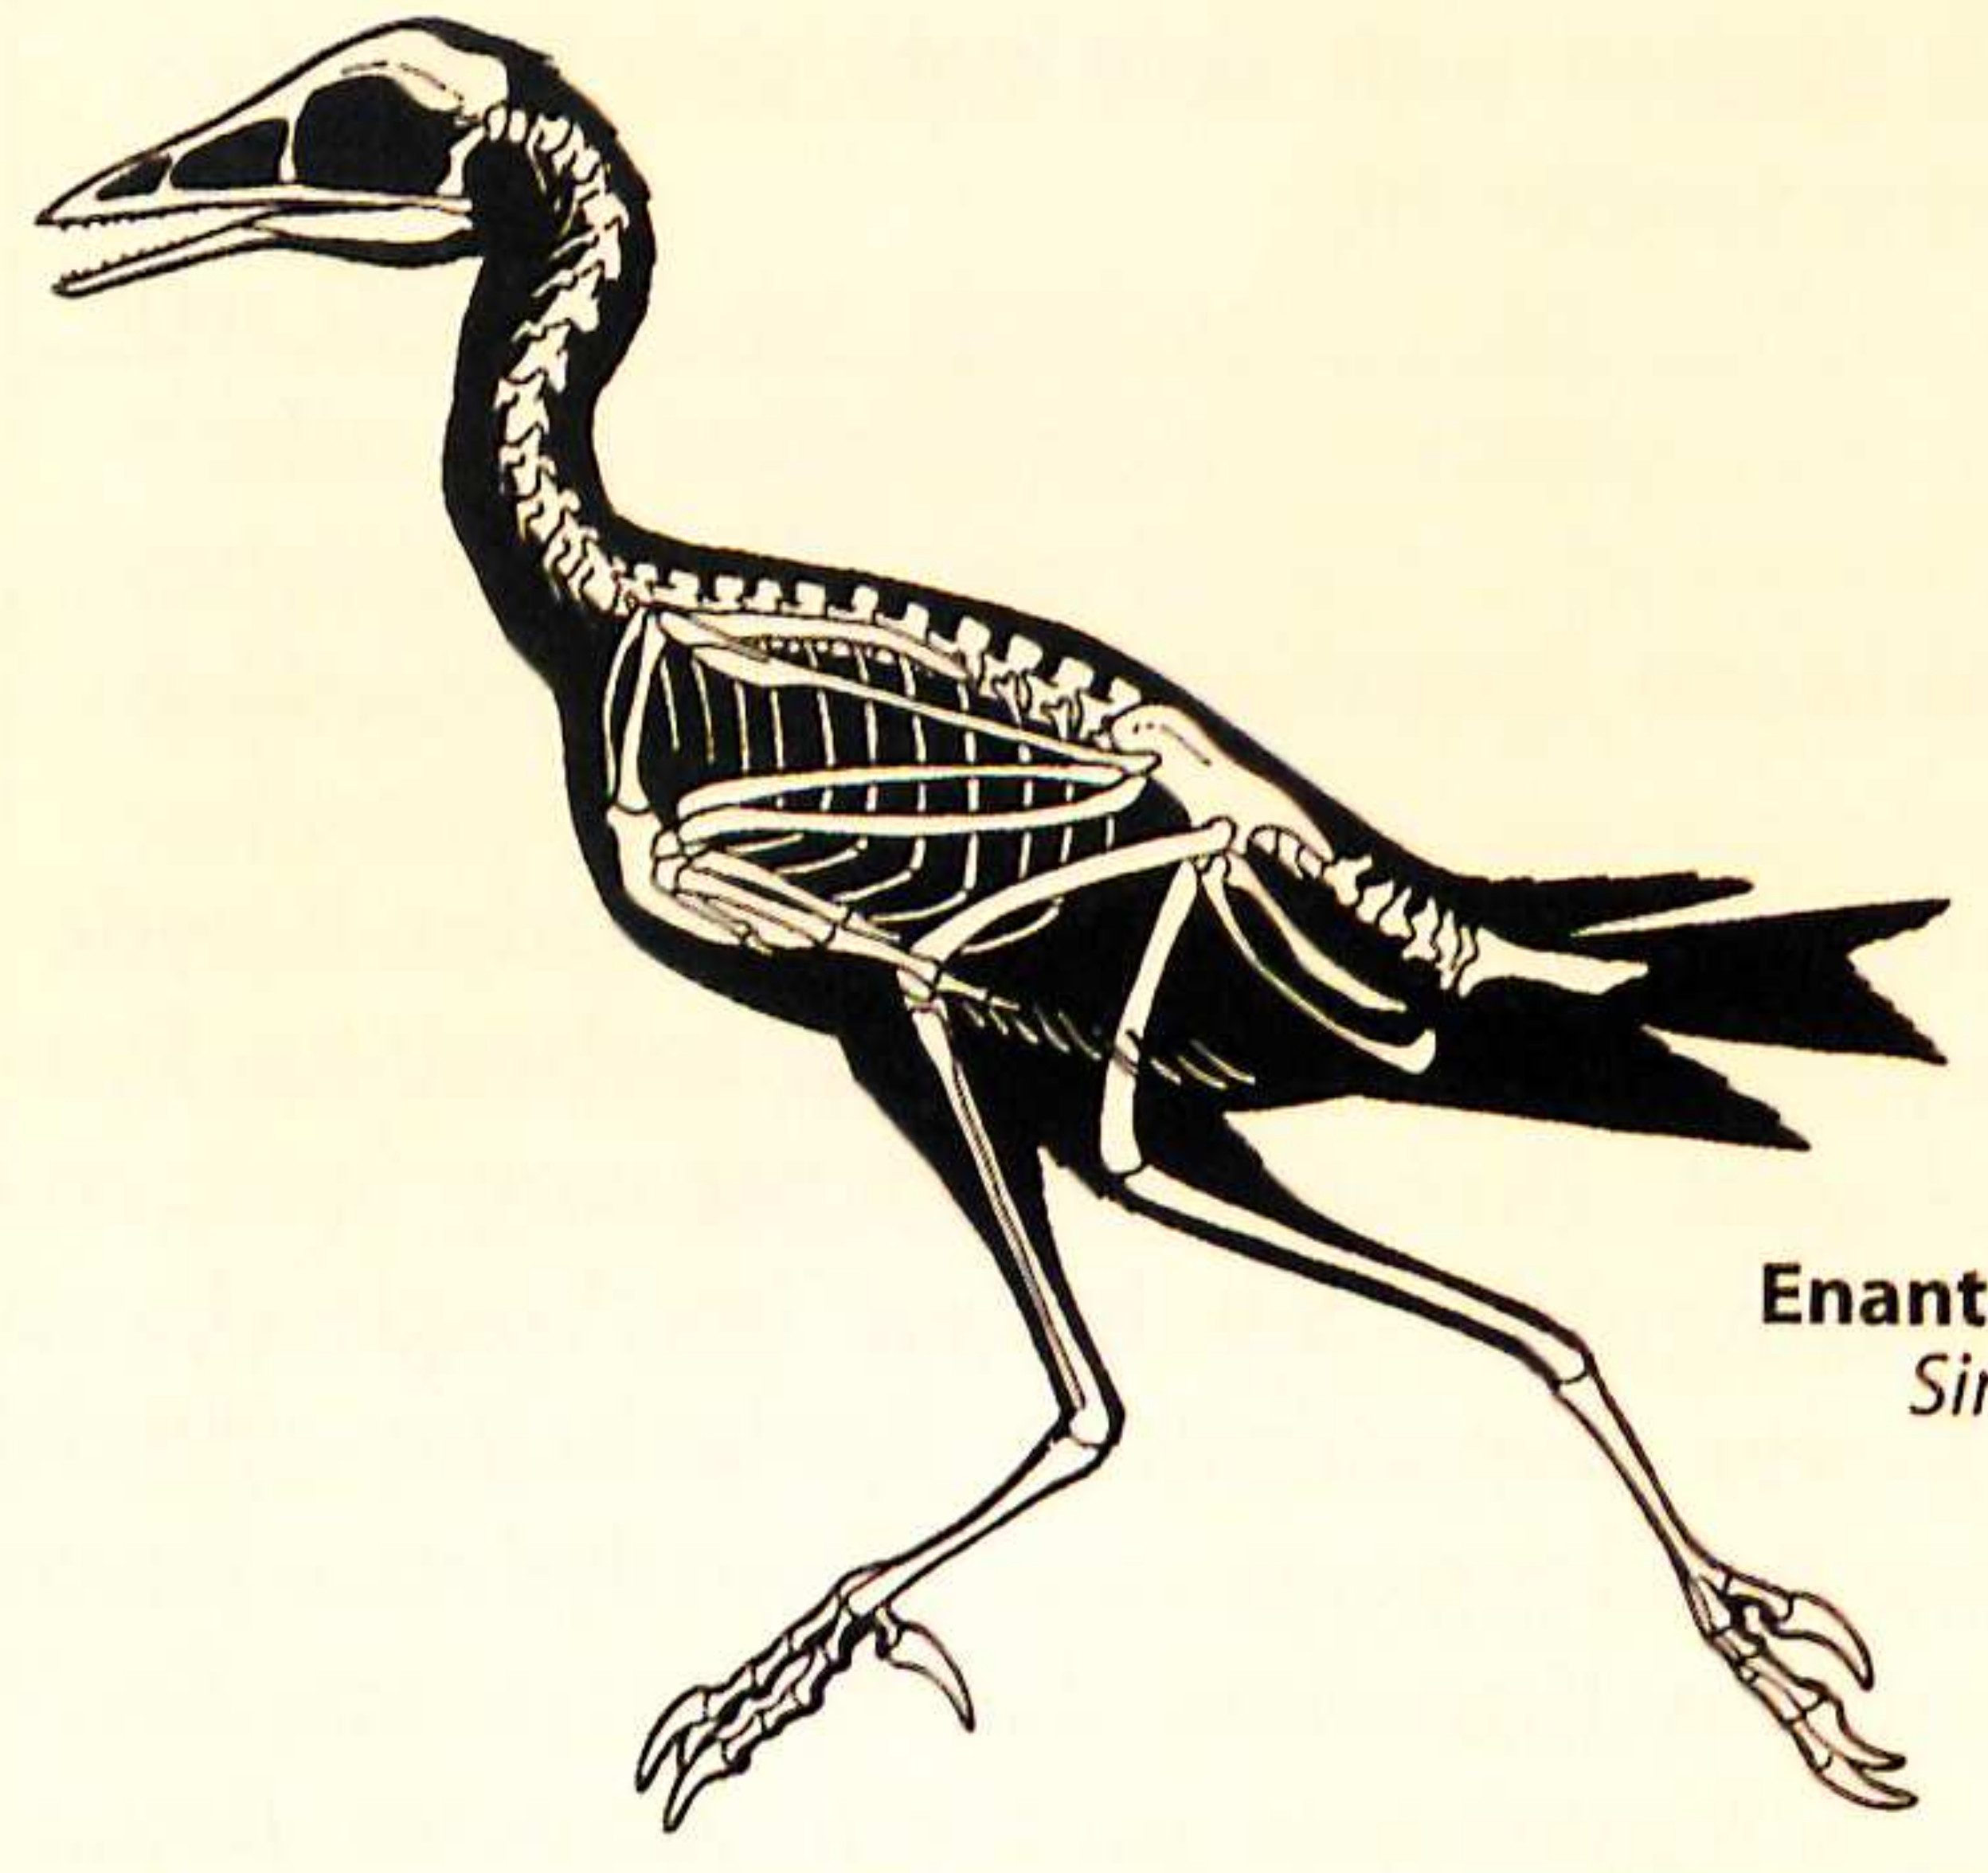
\includegraphics[width=0.2\textwidth]{../PCA/Skelettbilder_klein/Sinornis.jpg}}~
\subfloat[Stegosaurus]{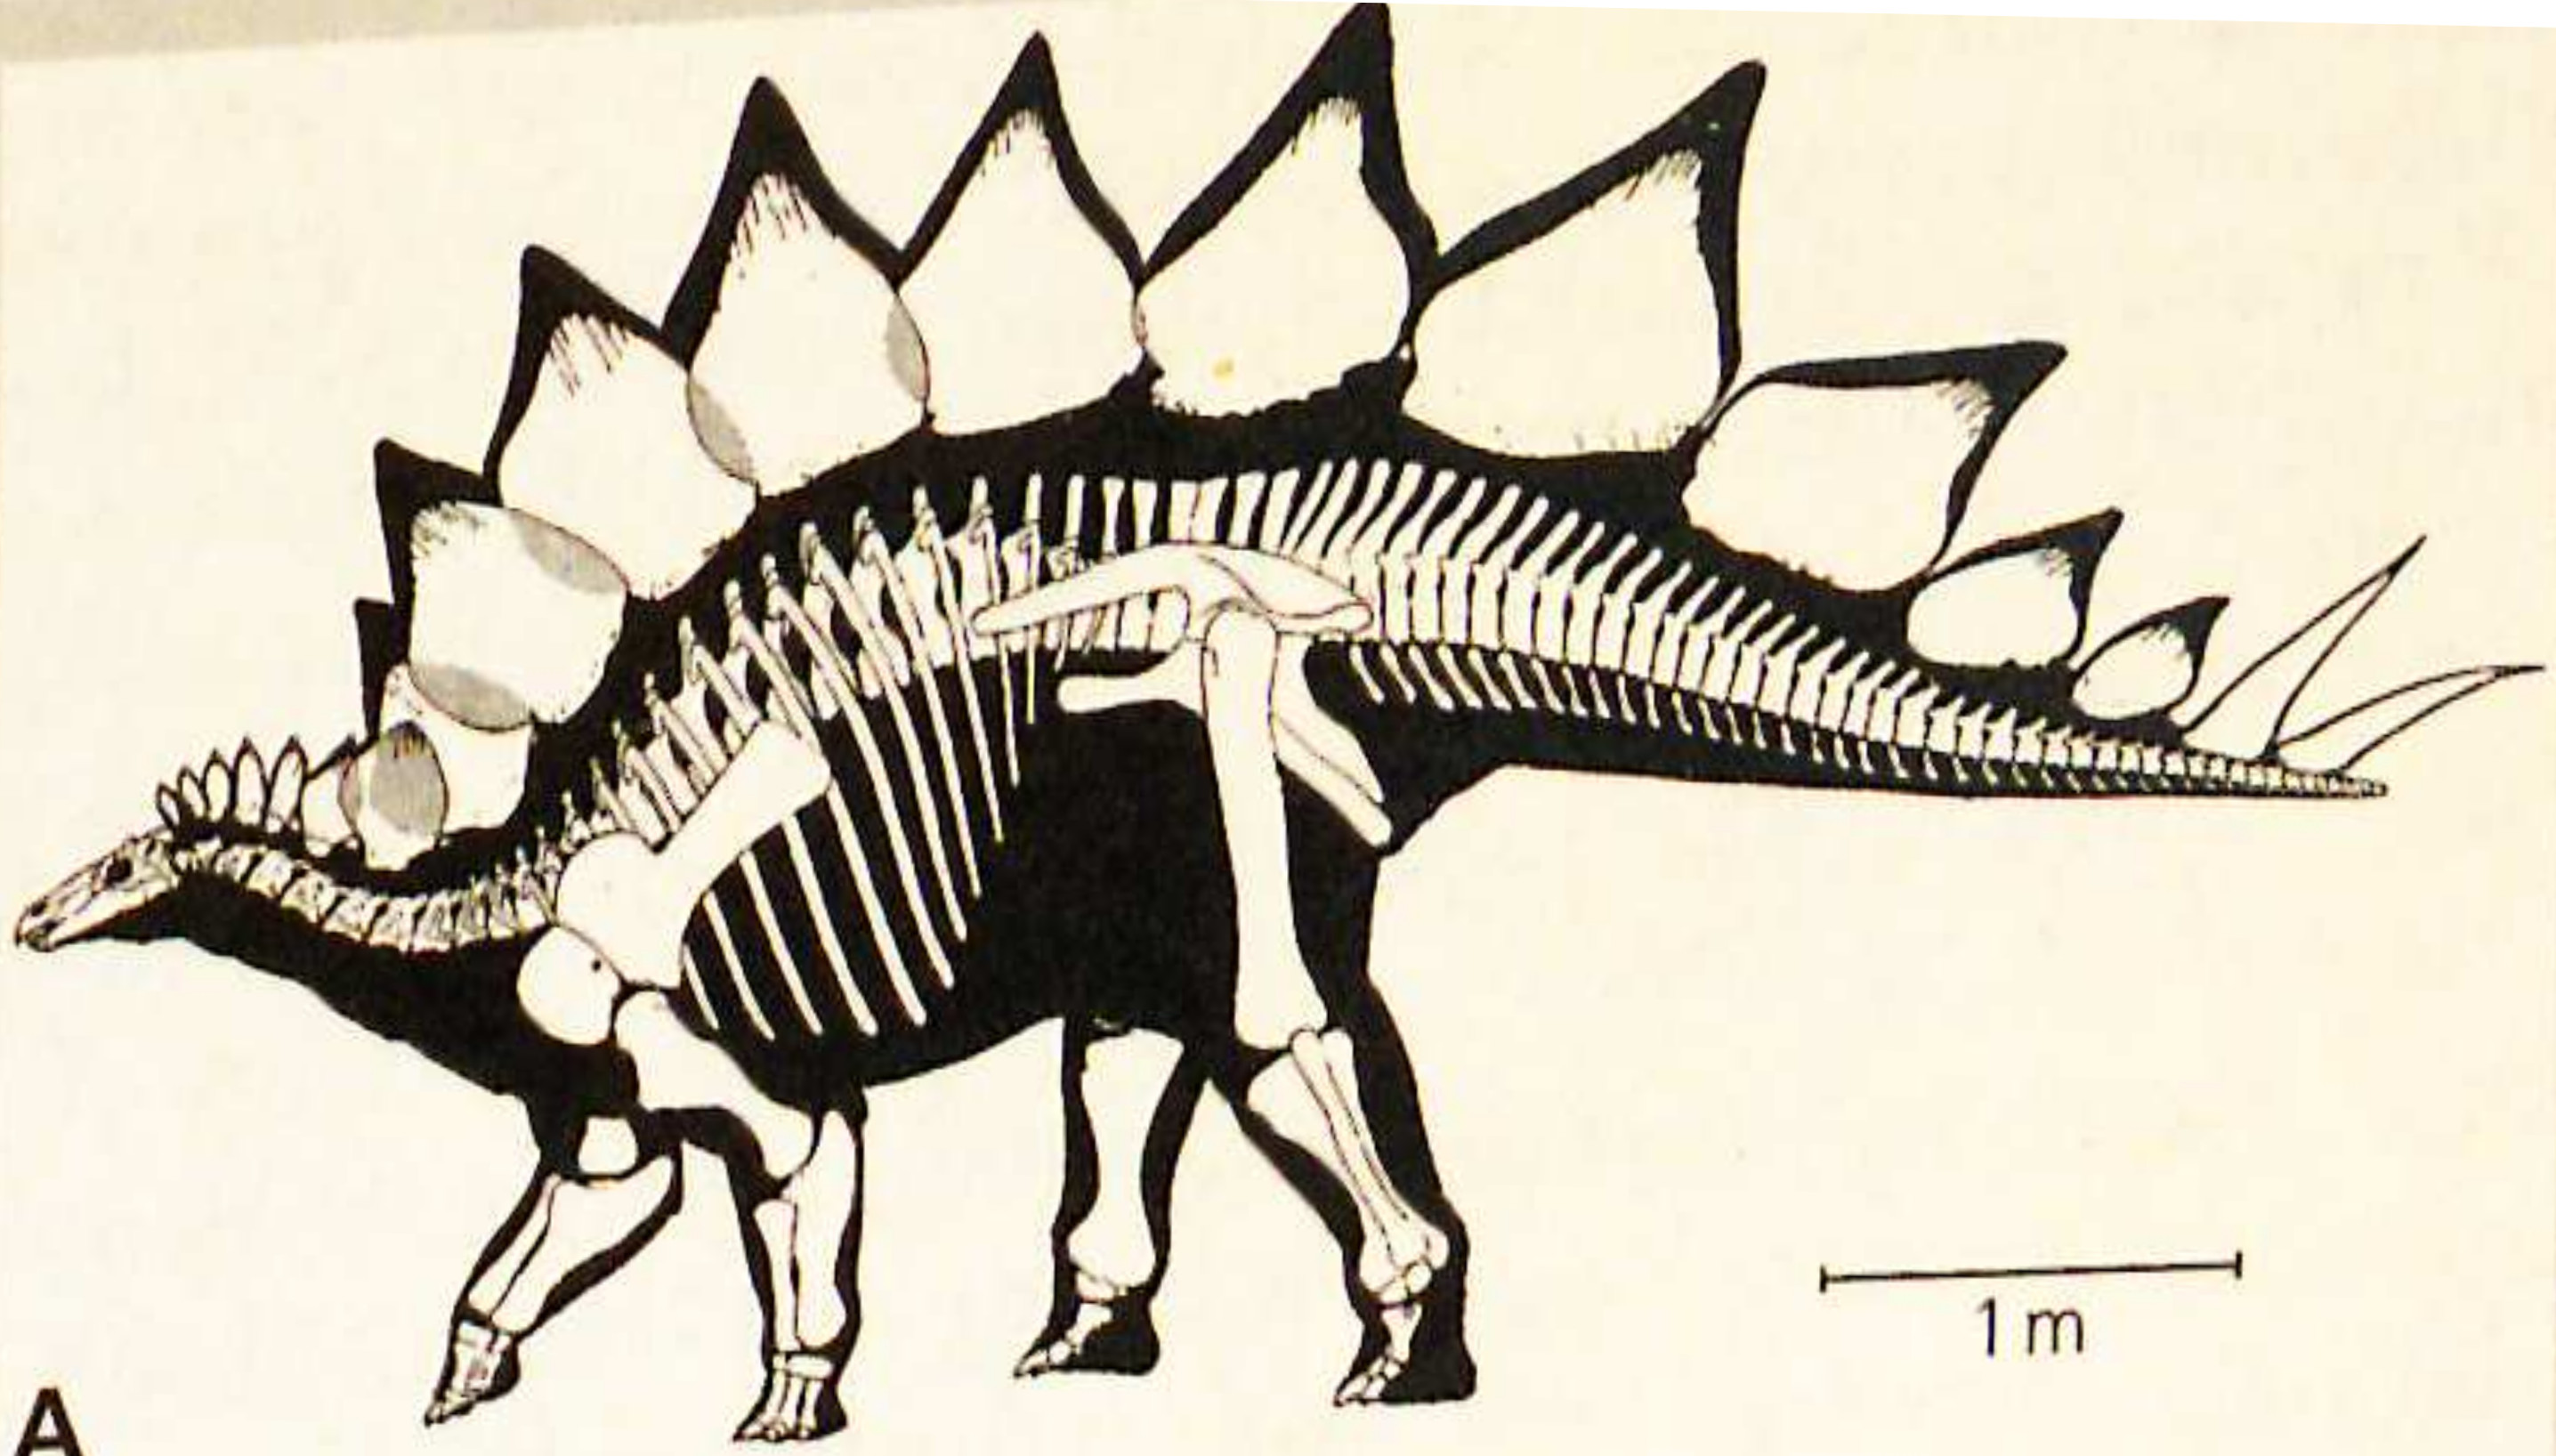
\includegraphics[width=0.2\textwidth]{../PCA/Skelettbilder_klein/Stegosaurus.jpg}}~
\subfloat[Strauss]{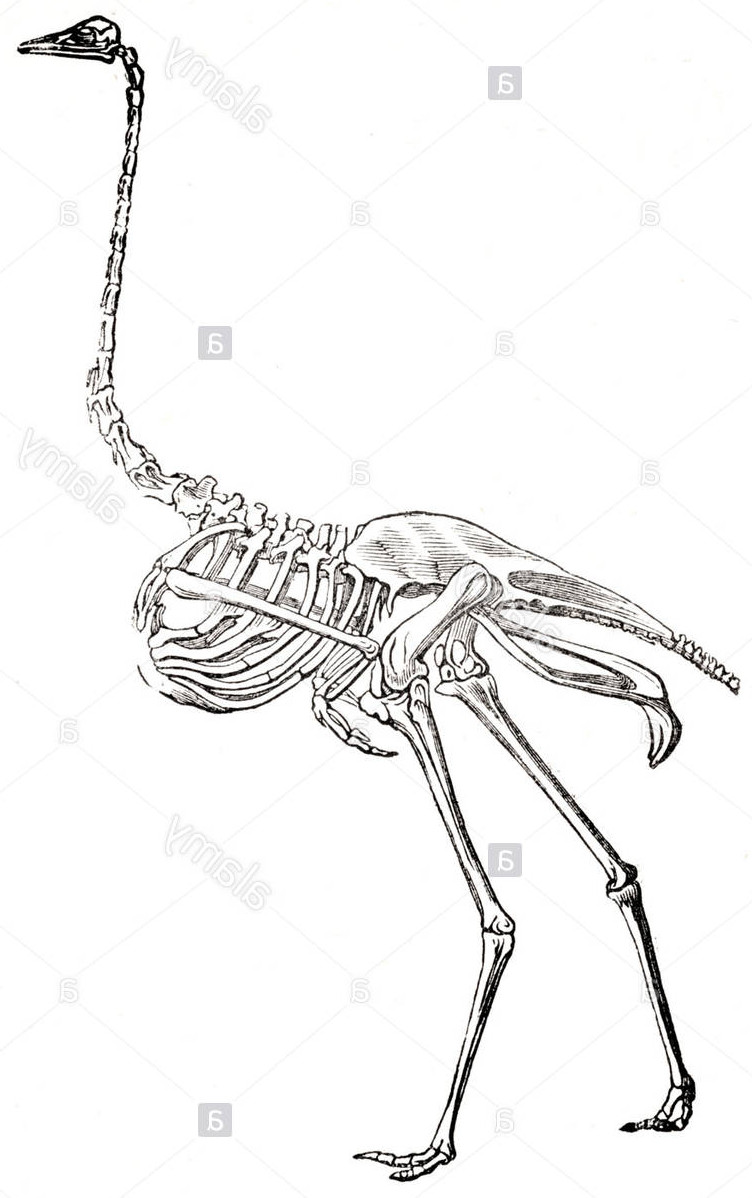
\includegraphics[width=0.2\textwidth]{../PCA/Skelettbilder_klein/Strauss.jpg}}~
\subfloat[Taube]{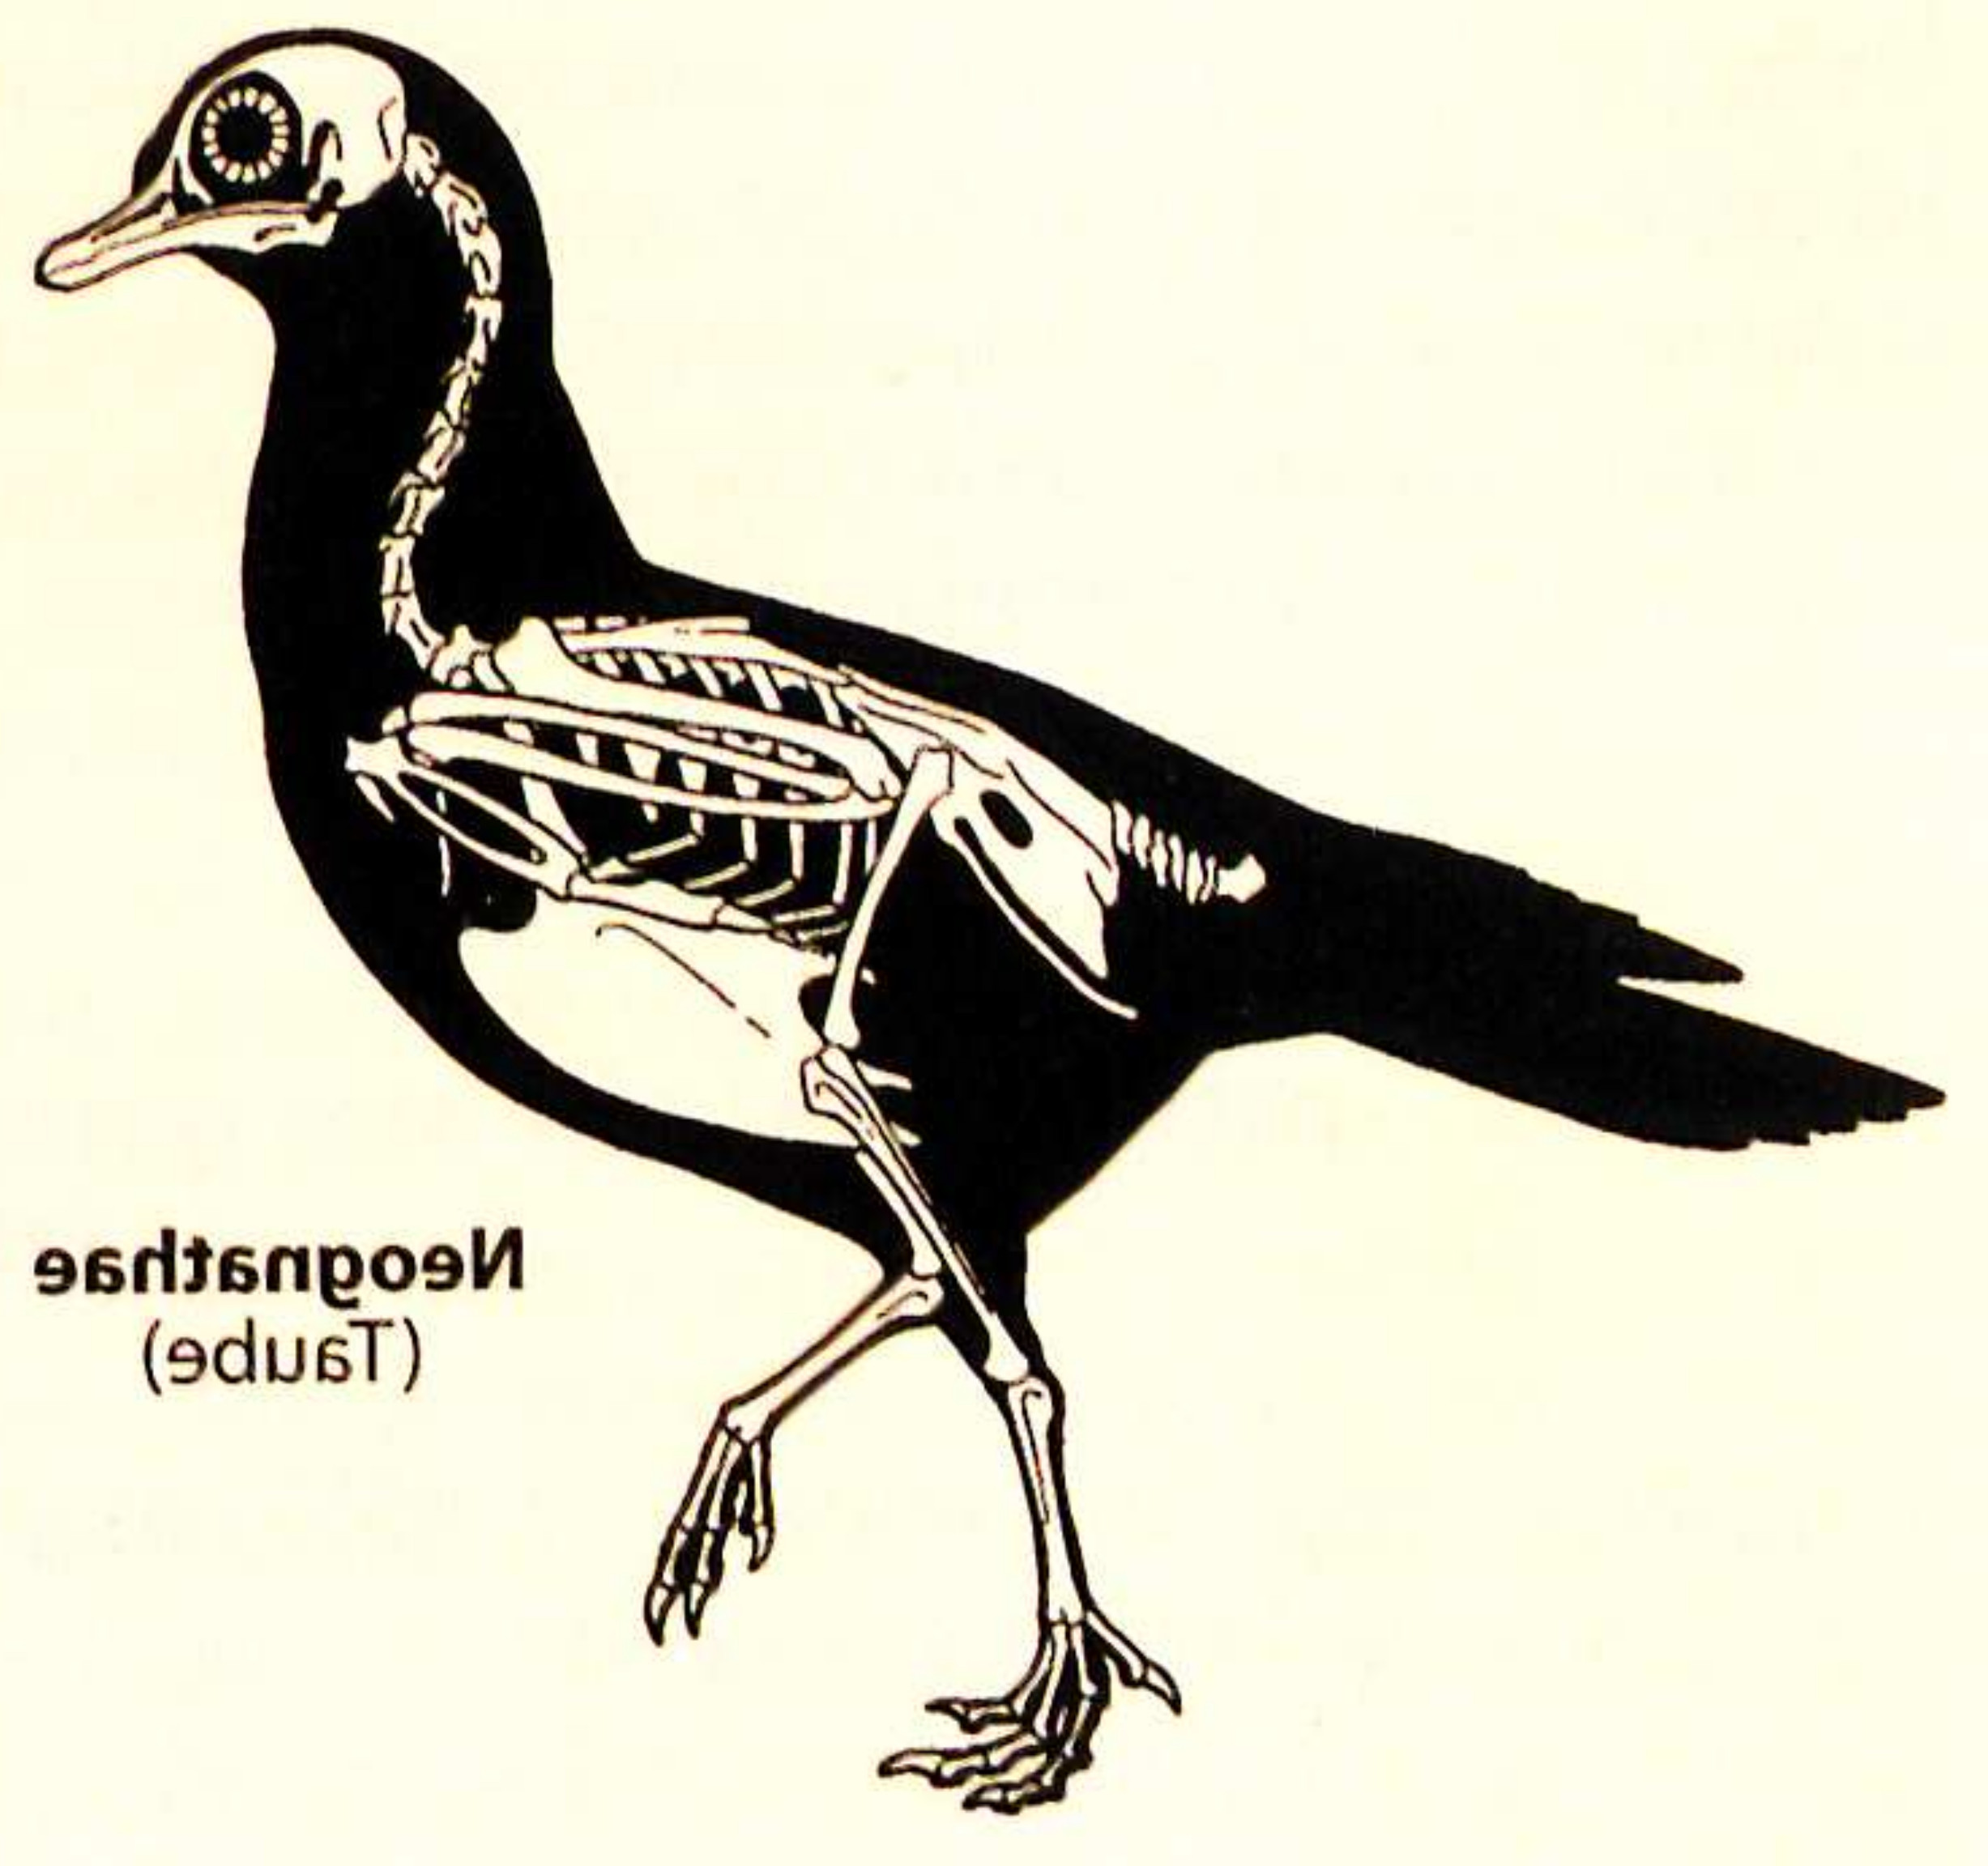
\includegraphics[width=0.2\textwidth]{../PCA/Skelettbilder_klein/Taube.jpg}}~
\subfloat[Thrinaxodon]{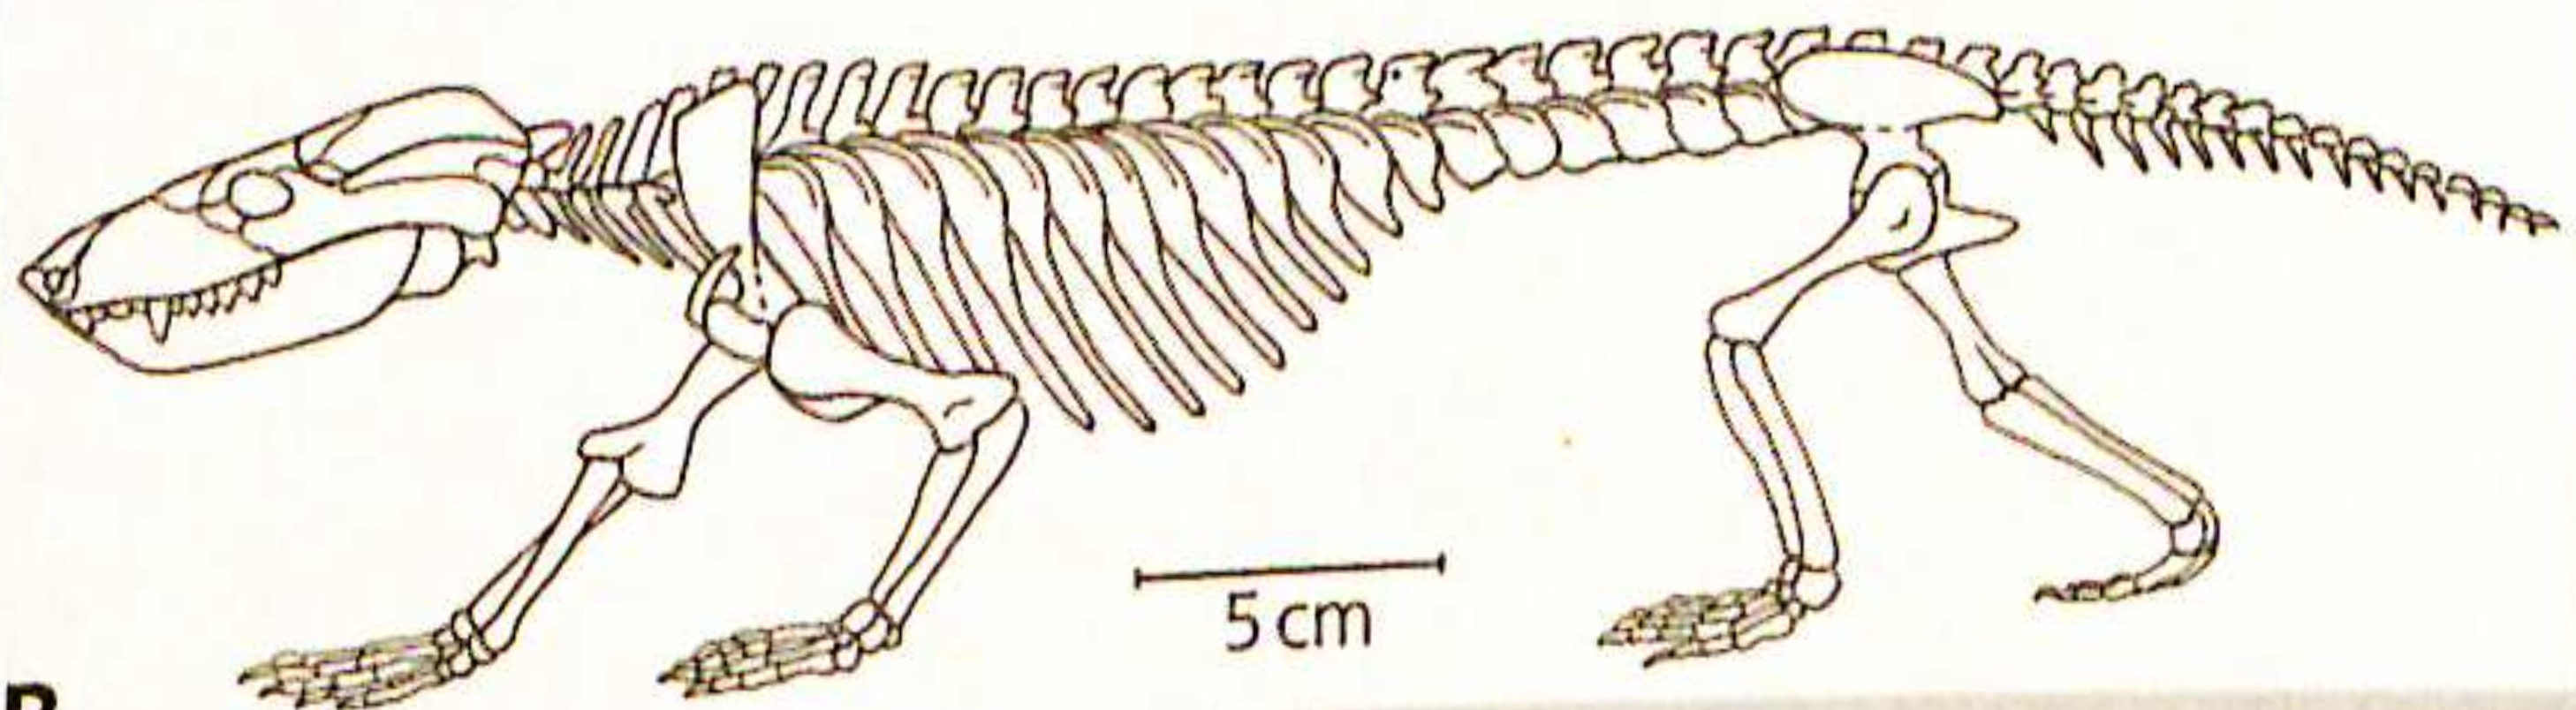
\includegraphics[width=0.2\textwidth]{../PCA/Skelettbilder_klein/Thrinaxodon.jpg}}
\\
\subfloat[Triceratops]{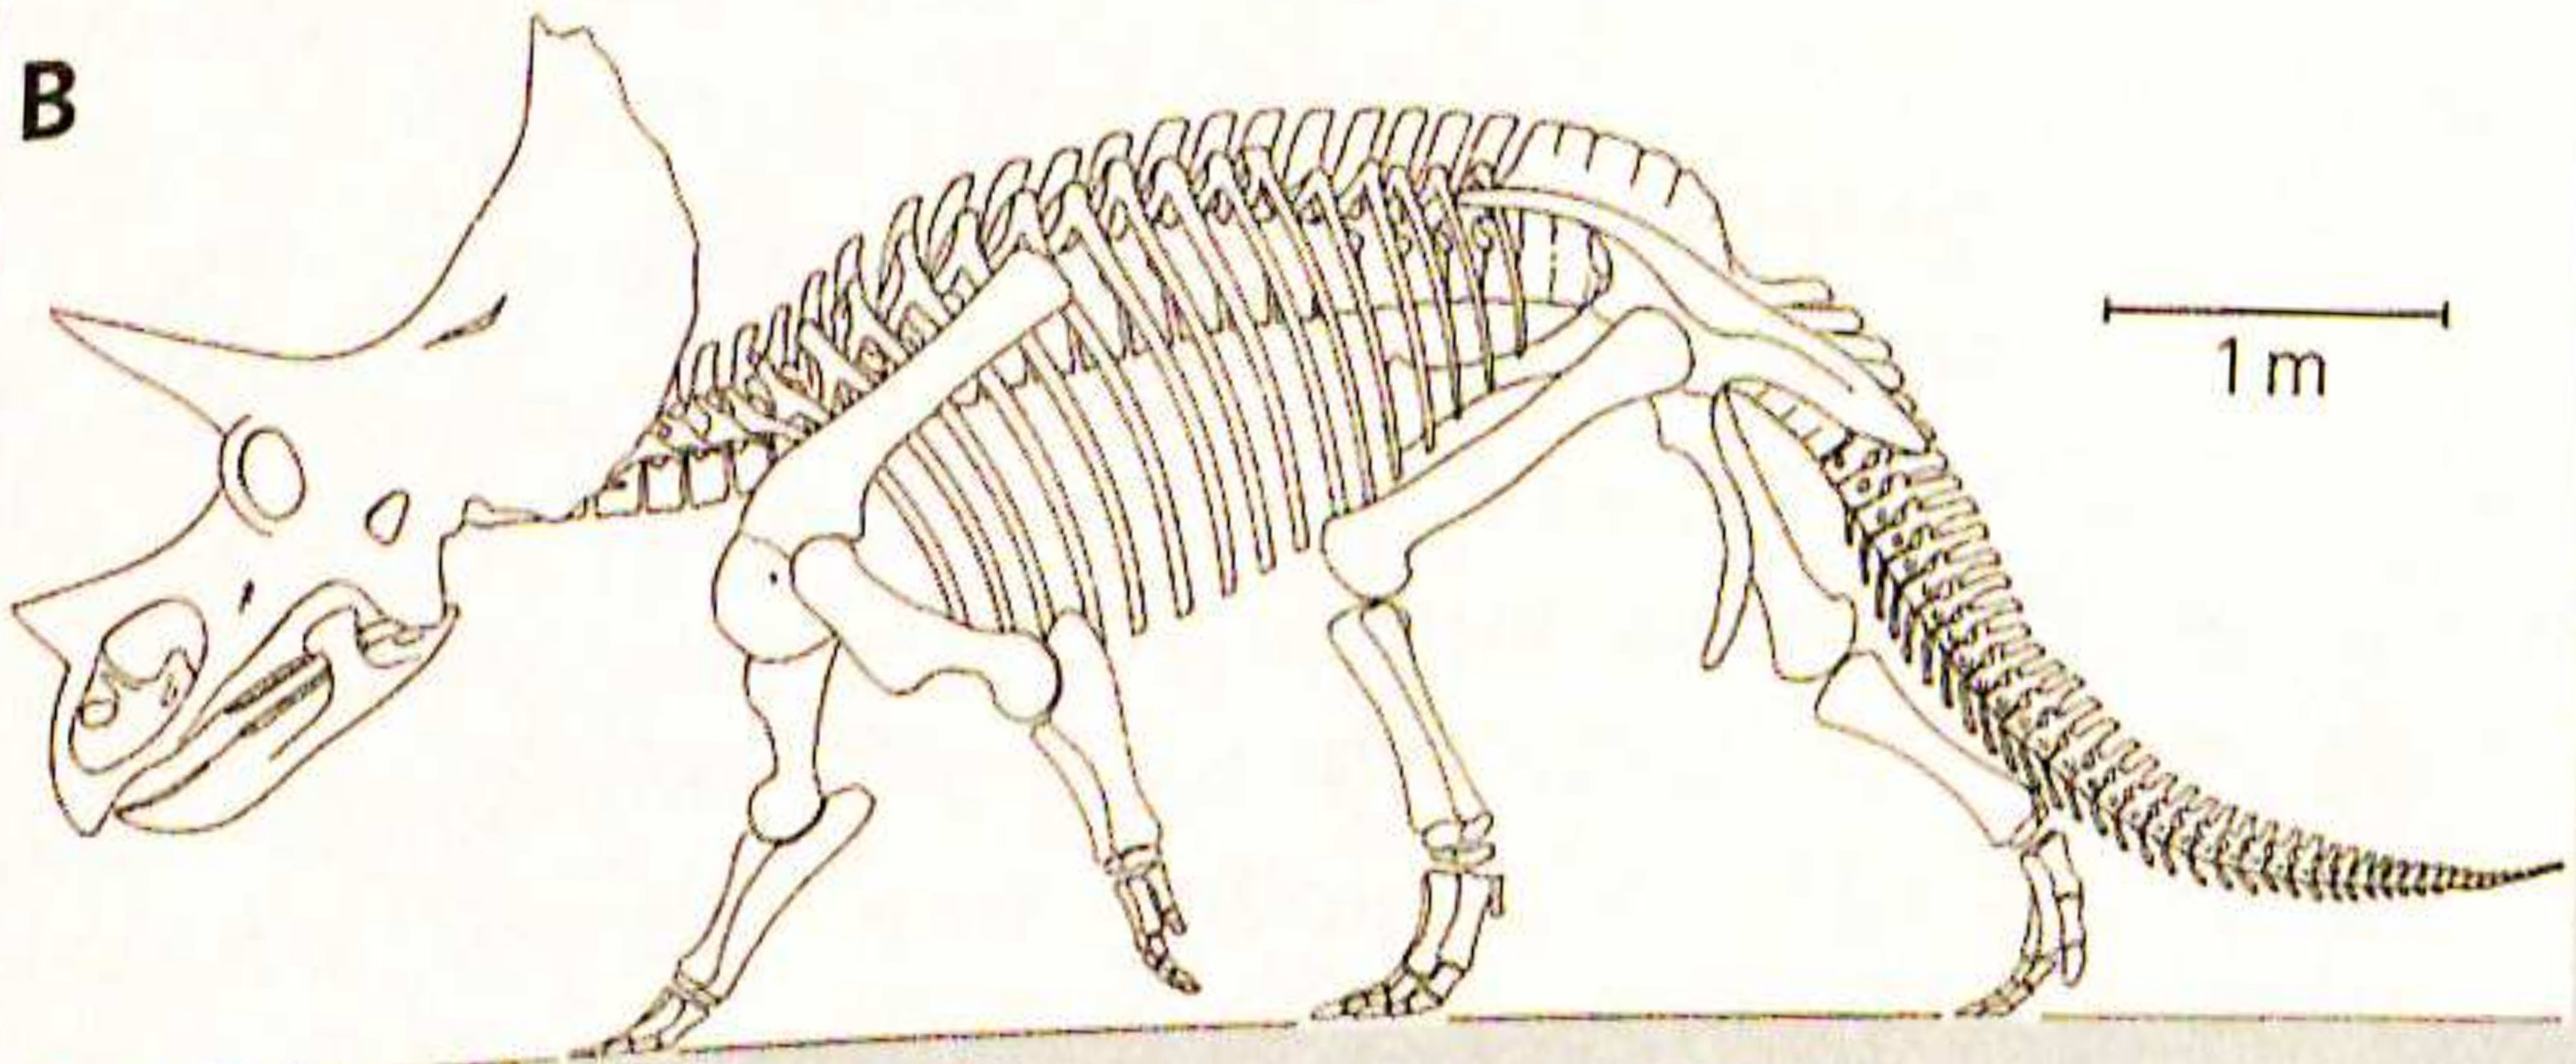
\includegraphics[width=0.2\textwidth]{../PCA/Skelettbilder_klein/Triceratops.jpg}}~
\subfloat[Tyrannosaurus Rex]{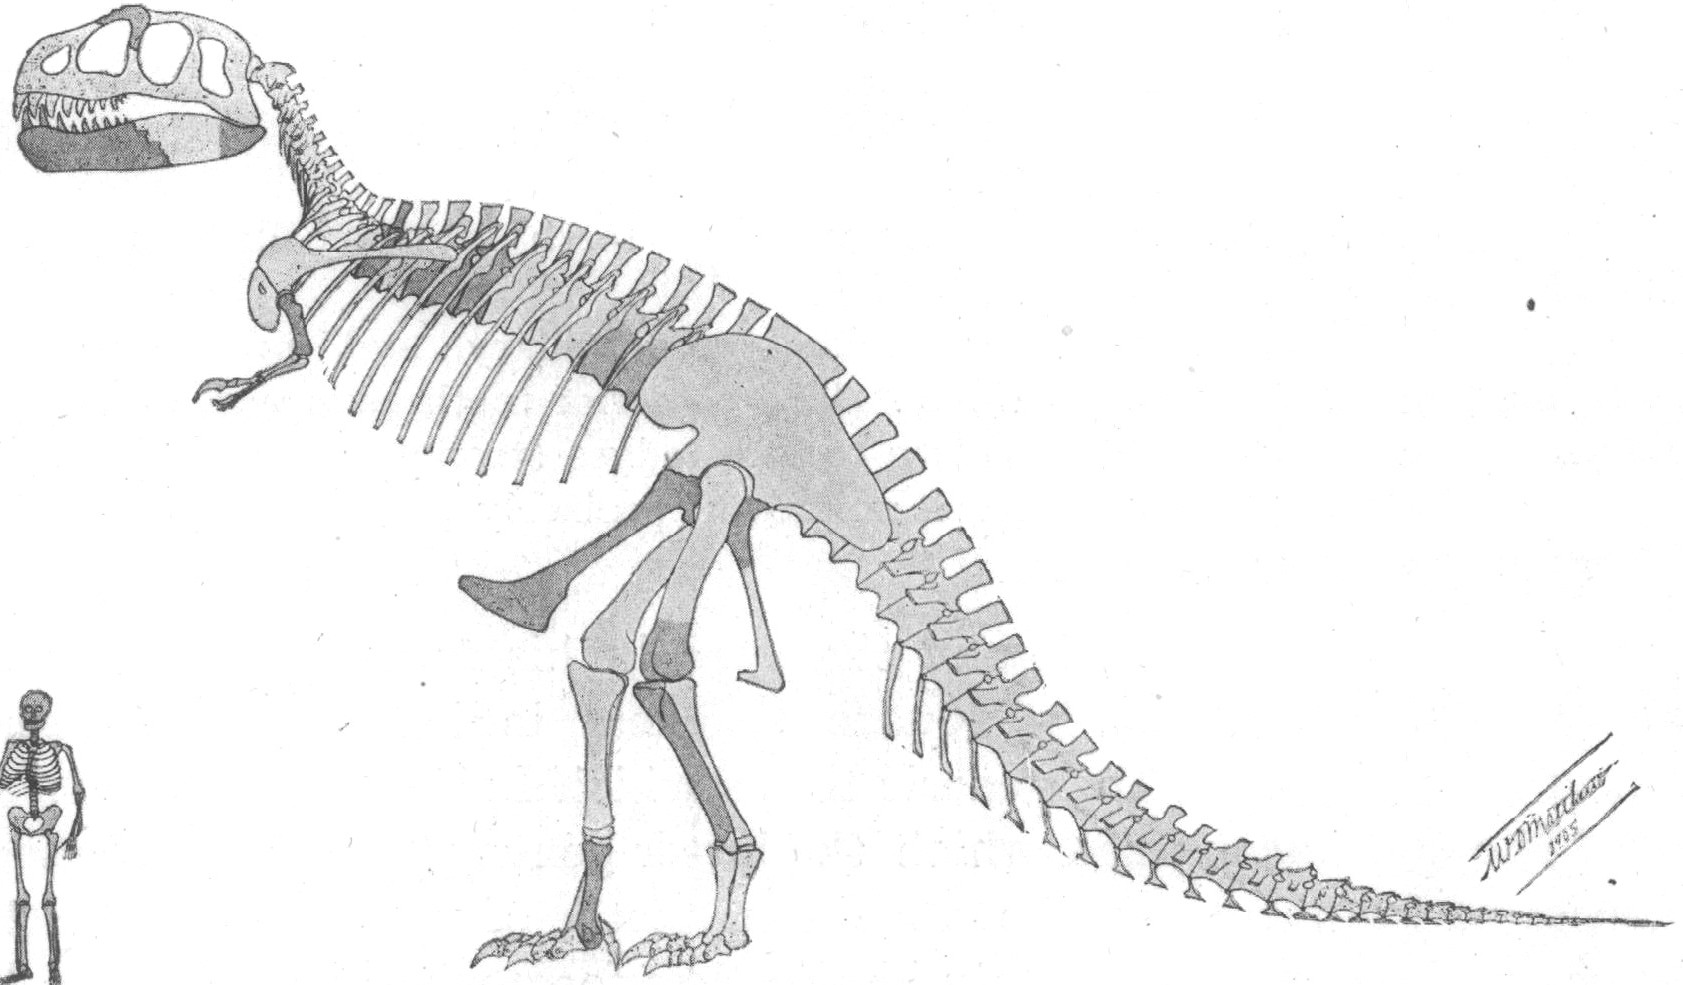
\includegraphics[width=0.2\textwidth]{../PCA/Skelettbilder_klein/Tyrannosaurus_Rex.jpg}}~
\subfloat[Urpferdchen]{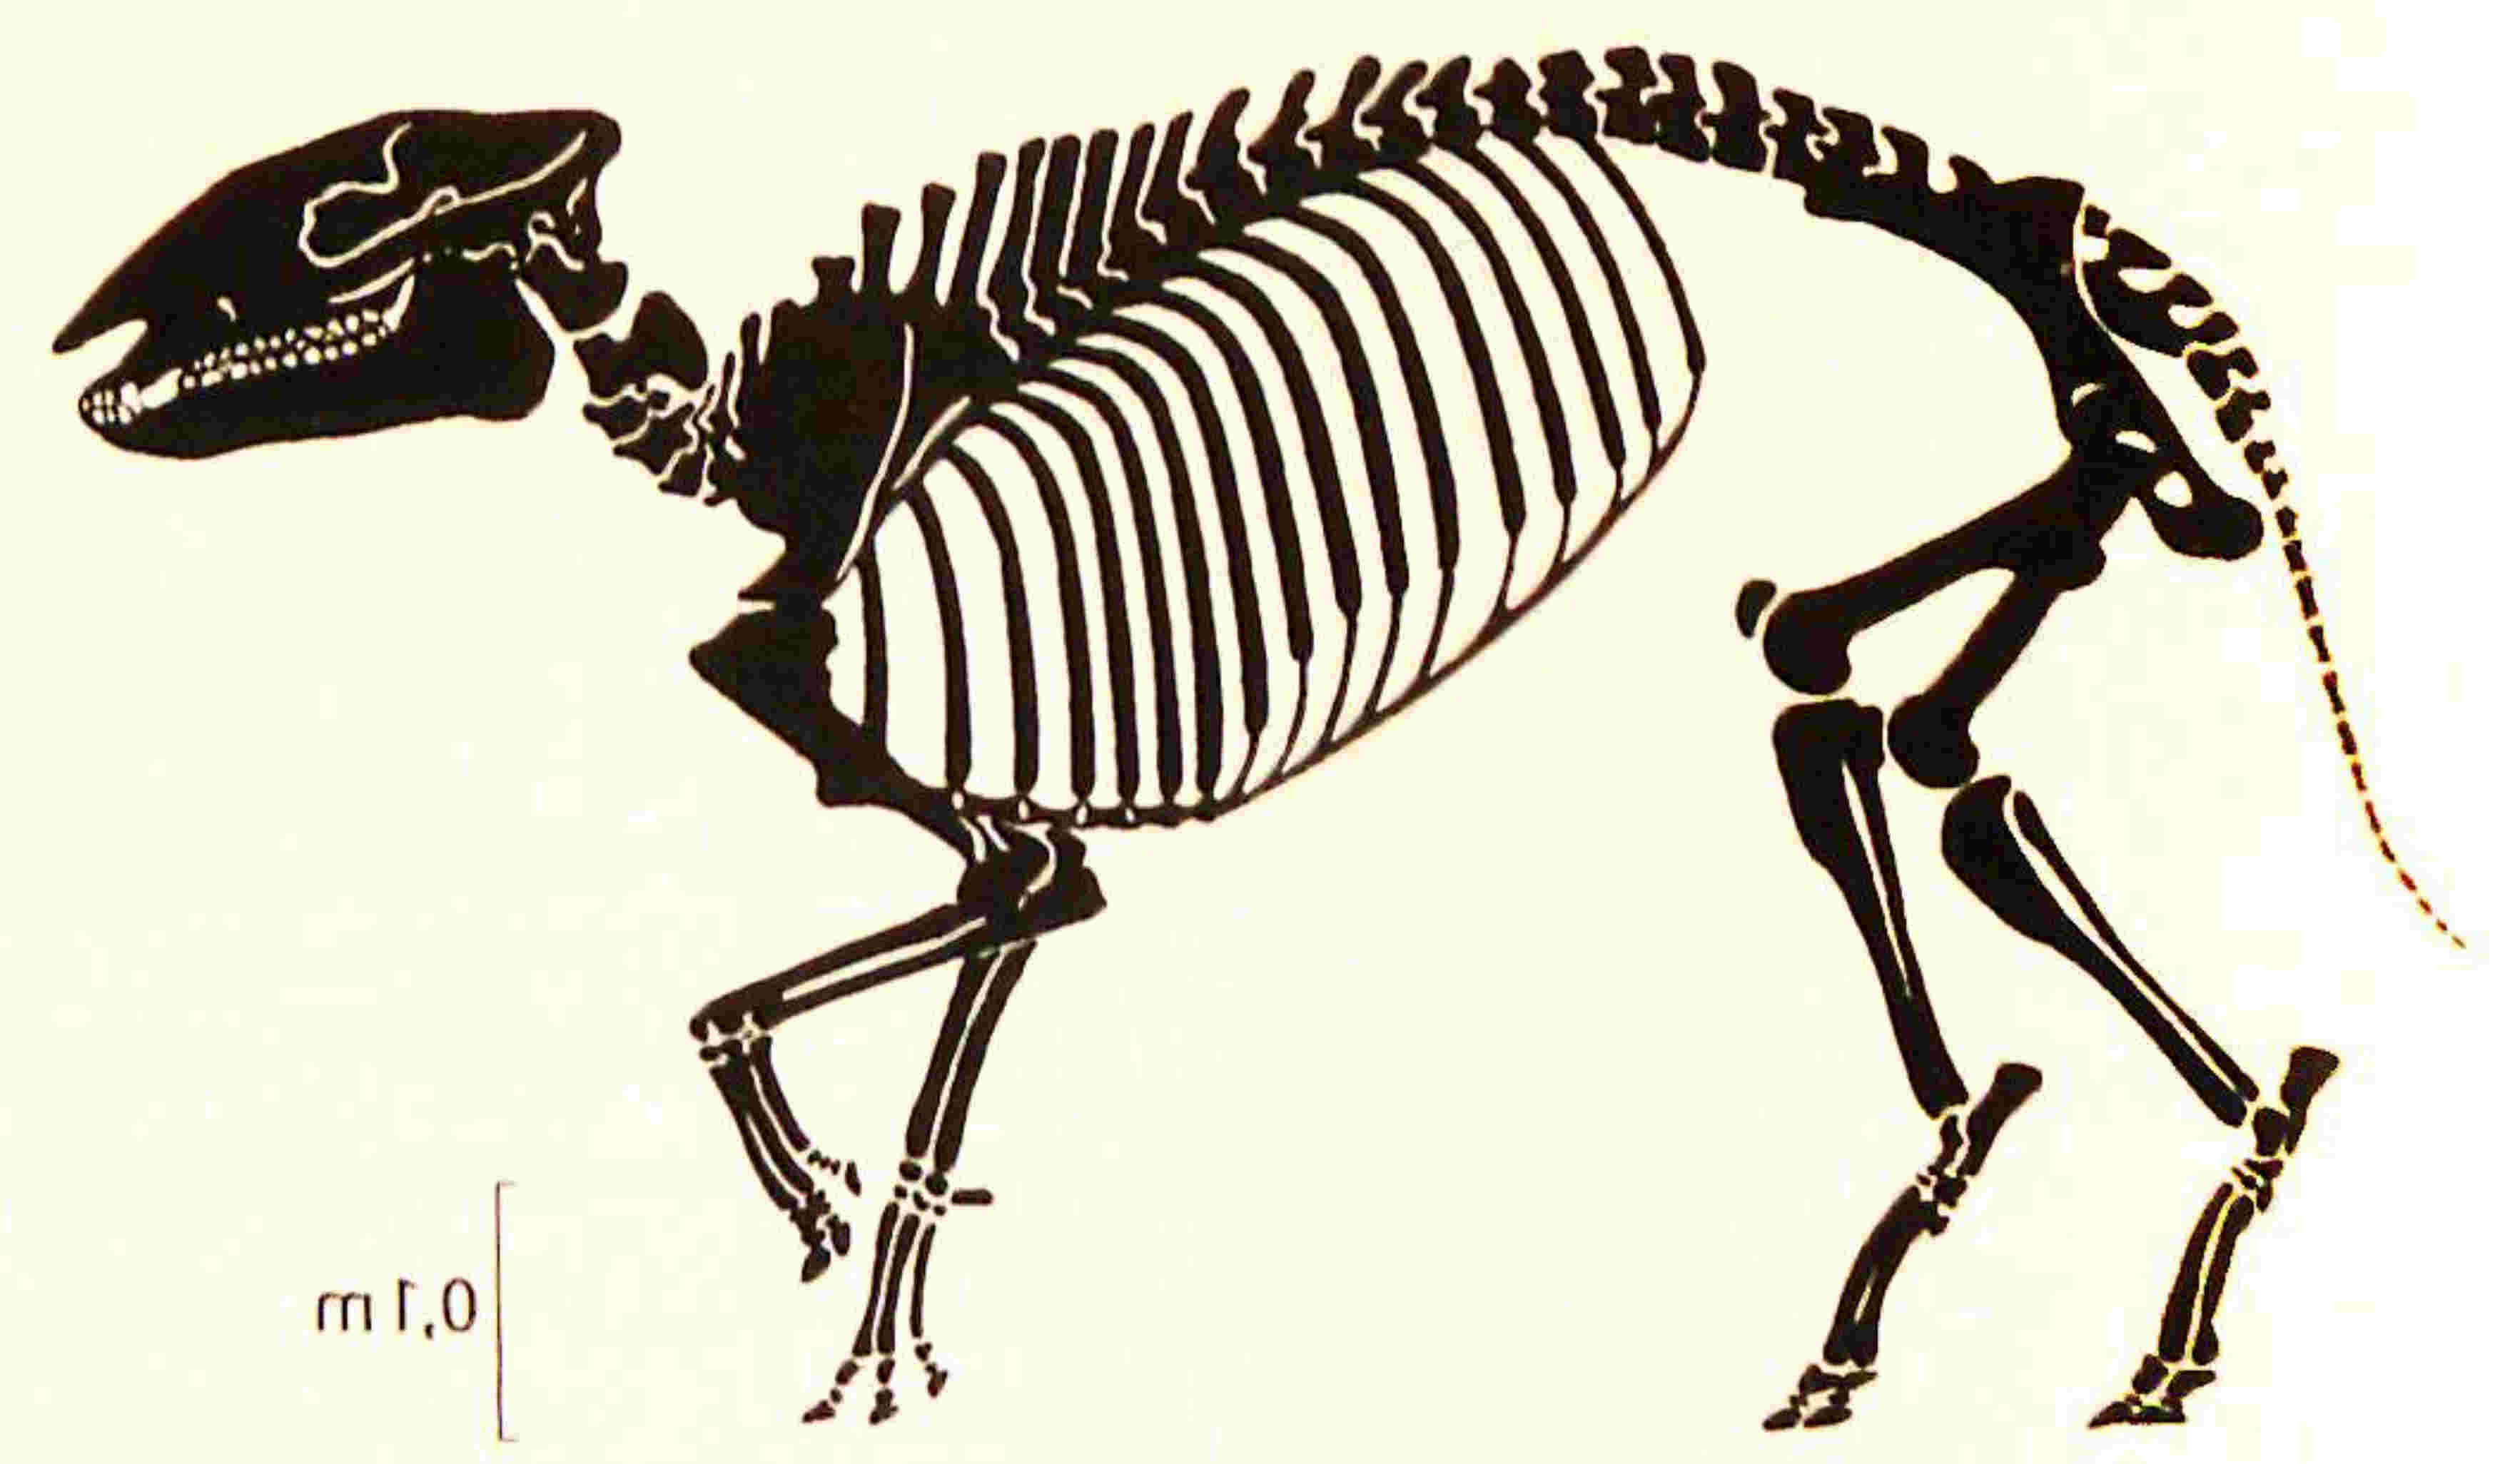
\includegraphics[width=0.2\textwidth]{../PCA/Skelettbilder_klein/Urpferdchen.jpg}}


\caption{Alle Bilder, die als Eingabe für die PCA verwendet wurden.}
\label{all_images}
\end{figure}


 
 \subsection{Gewichte}
 \label{appendix_pca_weight}
 
 \begin{itemize}
  \item Afrikanischer Elefant 4000kg, \url{https://de.upali.ch/gewicht-und-grosse/}
  \item Afrikanischer Strauß bis 135kg, \url{https://de.wikipedia.org/wiki/Afrikanischer_Strau\%C3\%9F}
  \item Amerikanischer Flussbarsch 2kg, \url{http://tierdoku.com/index.php?title=Amerikanischer_Flussbarsch}
  \item Archaeopteryx 1kg, \url{https://de.wikipedia.org/wiki/Archaeopteryx}
  \item Blauwal 120 Tonnen, \url{http://tierdoku.com/index.php?title=Blauwal}, "`das schwerste bekannte Tier der Erdgeschichte"' \url{https://de.wikipedia.org/wiki/Blauwal}
  \item Brachiosaurus 23-44 Tonnen, \url{https://de.wikipedia.org/wiki/Brachiosaurus}
  \item Chamäleon 0,1-2kg, \url{https://www.tierchenwelt.de/echsen/128-chamaeleon.html}
  \item Dimetrodon 250kg, \url{https://de.wikipedia.org/wiki/Dimetrodon}
  \item Dromedar 300-700kg, \url{https://de.wikipedia.org/wiki/Dromedar}
  \item Durschnittsgewicht (Warmblut-)Pferd 600 kg, \url{https://www.reitarena.com/de/blog/blog-post/2015/03/03/das-pferd-grundlegende-fakten.html}
  \item Elster 0,2kg, \url{https://de.wikipedia.org/wiki/Elster}
  \item Forelle 10-50kg (je nach Art), \url{https://de.wikipedia.org/wiki/Forelle}
  \item Frosch 10g, \url{http://www.biologie-schule.de/frosch-steckbrief.php}
  \item Gämse 25-50kg, \url{https://de.wikipedia.org/wiki/G\%C3\%A4mse}
  \item Girafffe bis 2 Tonnen, \url{https://www.tierchenwelt.de/huftiere/73-giraffe.html}
  \item Gnu 140-250kg, \url{https://de.wikipedia.org/wiki/Gnus}
  \item Grönlandwal 50-100 Tonnen, \url{https://de.wikipedia.org/wiki/Gr\%C3\%B6nlandwal}
  \item Ichthyornis 0.3kg, \url{http://dinodata.de/animals/birds/pages_i/ichthyornis.php}
  \item Ichthyosaurus 90kg, \url{https://www.tiere-online.de/sonstige-tiere/dinosaurier/ichthyosaurus/}
  \item Ichthyostega 80kg, \url{https://dinosaurierwelt.com/ichthyostega/}
  \item Kaffernbüffel 350-900kg, \url{https://de.wikipedia.org/wiki/Kaffernb\%C3\%BCffel}
  \item Känguru 2-90kg ,\url{https://de.wikipedia.org/wiki/K\%C3\%A4ngurus}
  \item Kaninchen je nach Art, ganz grob 1kg
  \item Klippschliefer 2-5kg, \url{https://de.wikipedia.org/wiki/Klippschliefer}
  \item Koboldmaki 0,1kg, \url{https://de.wikipedia.org/wiki/Koboldmakis}
  \item Krokodil 100-1000kg, \url{https://de.wikipedia.org/wiki/Krokodile}
  \item Landschildkröte je nach Art, grob 50kg
  \item Ohrenrobbe 25-500kg, \url{https://de.wikipedia.org/wiki/Ohrenrobben}
  \item Panzerspitzmaus 100g ,\url{https://de.wikipedia.org/wiki/Panzerspitzmaus}
  \item Parasaurolophus walkeri 4-5 Tonnen, \url{http://tierdoku.com/index.php?title=Parasaurolophus_walkeri}
  \item Peloneustes philarchus 100kg, \url{https://de.wikipedia.org/wiki/Peloneustes}
  \item Pottwal bis 50 Tonnen, \url{https://de.wikipedia.org/wiki/Pottwal}
  \item Rothirsch 80-350kg, \url{https://de.wikipedia.org/wiki/Rothirsch}
  \item Schlange bis 100kg bei Riesenschlangen, \url{https://de.wikipedia.org/wiki/Schlangen}
  \item Schwan 14kg, \url{https://de.wikipedia.org/wiki/Schw\%C3\%A4ne}
  \item Schwein 100kg, \url{https://de.wikipedia.org/wiki/Hausschwein}
  \item Seehund 100-150kg, \url{https://de.wikipedia.org/wiki/Seehund}
  \item Sinornis 20g, \url{http://dinodata.de/animals/birds/pages_s/sinornis.php}
  \item Stegosaurus 4,5 Tonnen, \url{https://de.wikipedia.org/wiki/Stegosaurus}
  \item Taube je nach Art, grob 1-2kg
  \item Thrinaxodon Reptil "`ein paar Pfund"', \url{https://www.thoughtco.com/thrinaxodon-1091887}
  \item Triceratops 6-12 Tonnen, \url{https://de.wikipedia.org/wiki/Triceratops}
  \item Tyrannosaurus 9 Tonnen, \url{https://de.wikipedia.org/wiki/Tyrannosaurus}
  \item Urpferdchen (Propalaeotherium) 30kg, \url{https://de.wikipedia.org/wiki/Propalaeotherium}
 \end{itemize}
 

% --------------
% Erhobene Werte
% --------------

  \begin{figure}
   \subfloat[Erster Punkt des Halses]{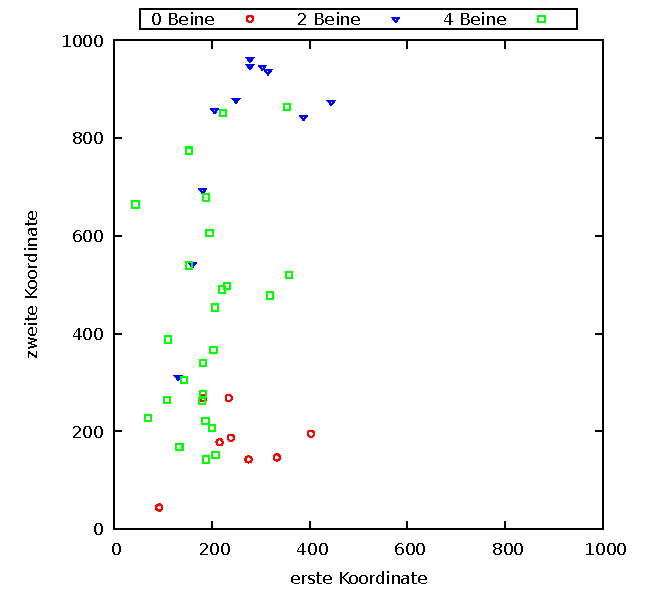
\includegraphics[width=0.3\textwidth]{../PCA/gnuplot/results_with_leg_tag/input_neck1.pdf}}
   \qquad
   \subfloat[Zweiter Punkt des Halses]{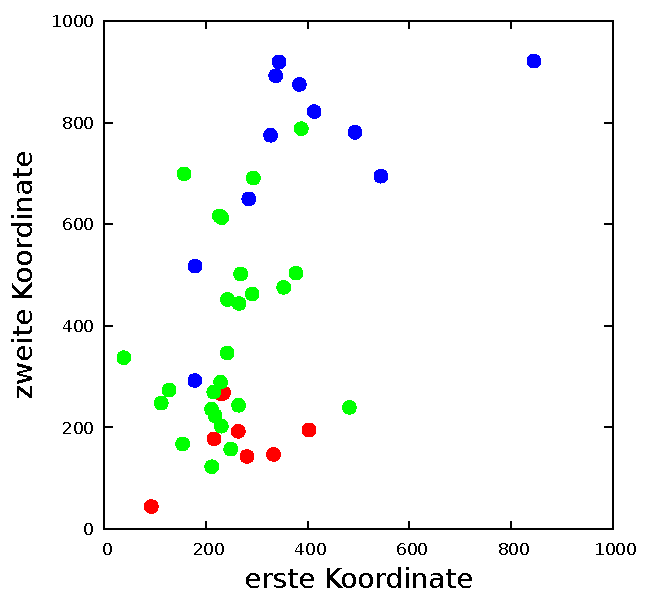
\includegraphics[width=0.3\textwidth]{../PCA/gnuplot/results_with_leg_tag/input_neck2.pdf}}
   \qquad
   \subfloat[Dritter Punkt des Halses]{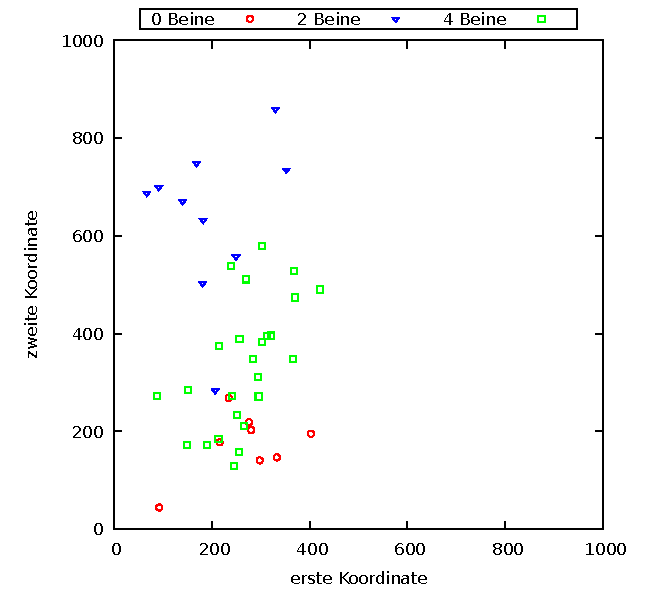
\includegraphics[width=0.3\textwidth]{../PCA/gnuplot/results_with_leg_tag/input_neck3.pdf}}
   \\
   \subfloat[Vierter Punkt des Halses \bzw erster Punkt des Rückens]{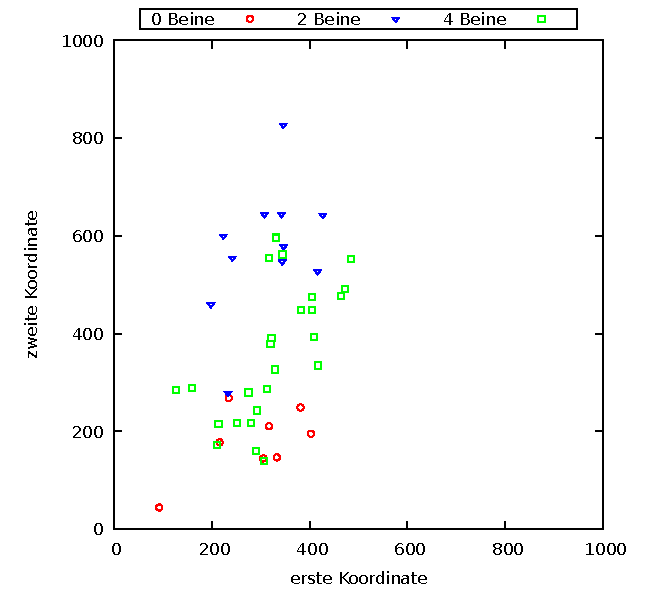
\includegraphics[width=0.3\textwidth]{../PCA/gnuplot/results_with_leg_tag/input_back1.pdf}}
   \qquad
   \subfloat[Zweiter Punkt des Rückens]{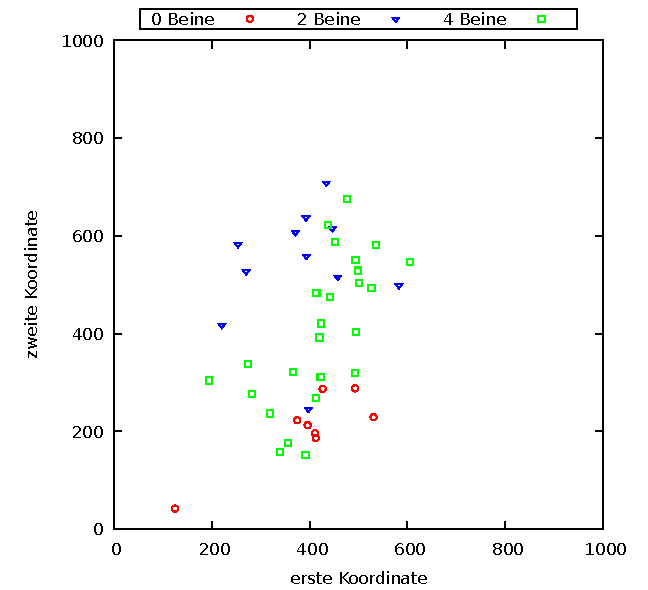
\includegraphics[width=0.3\textwidth]{../PCA/gnuplot/results_with_leg_tag/input_back2.pdf}}
   \qquad
   \subfloat[Dritter Punkt des Rückens]{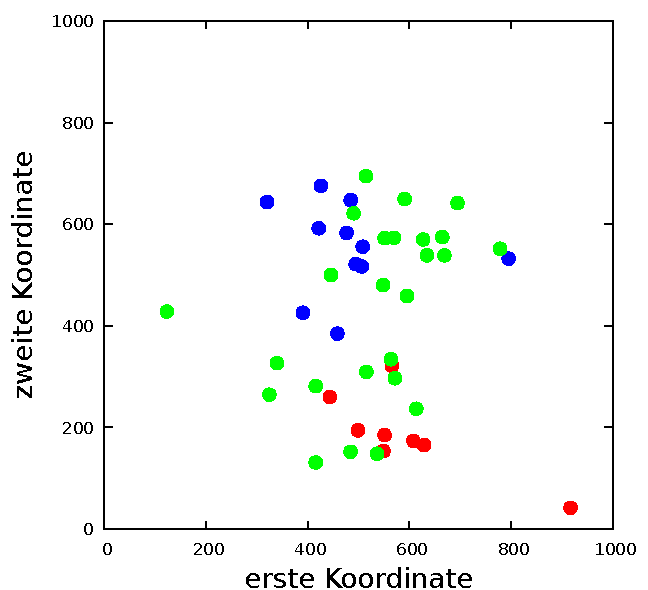
\includegraphics[width=0.3\textwidth]{../PCA/gnuplot/results_with_leg_tag/input_back3.pdf}}
   \\
   \subfloat[Vierter Punkt des Rückens \bzw erster Punkt des Schwanzes]{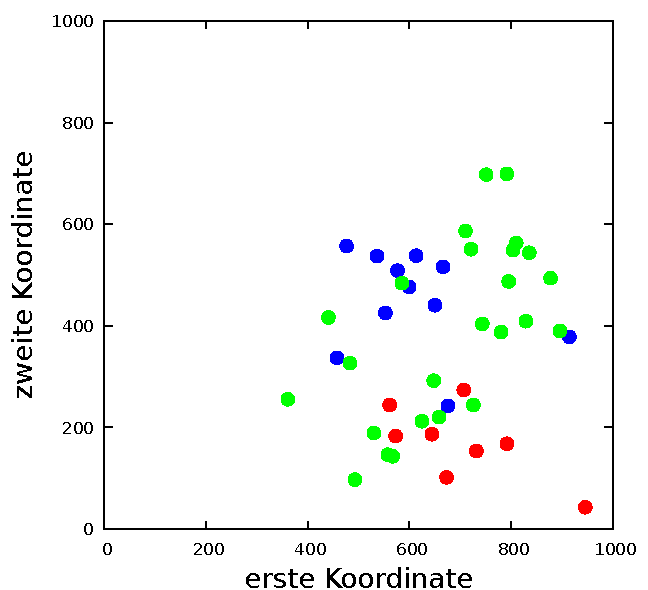
\includegraphics[width=0.3\textwidth]{../PCA/gnuplot/results_with_leg_tag/input_back4.pdf}}
   \qquad
   \subfloat[Zweiter Punkt des Schwanzes]{\includegraphics[width=0.3\textwidth]{../PCA/gnuplot/results_with_leg_tag/input_tail2.pdf}}
   \qquad
   \subfloat[Dritter Punkt des Schwanzes]{\includegraphics[width=0.3\textwidth]{../PCA/gnuplot/results_with_leg_tag/input_tail3.pdf}}
   \\
   \subfloat[Vierter Punkt des Schwanzes]{\includegraphics[width=0.3\textwidth]{../PCA/gnuplot/results_with_leg_tag/input_tail4.pdf}}
   \qquad
   \subfloat[Länge Ober- und Unterarm]{\includegraphics[width=0.3\textwidth]{../PCA/gnuplot/results_with_leg_tag/input_upper+lowerArm.pdf}}
   \qquad
   \subfloat[Länge Unterarm und Hand]{\includegraphics[width=0.3\textwidth]{../PCA/gnuplot/results_with_leg_tag/input_lowerArm+hand.pdf}}
   \phantomcaption
  \end{figure}
  \begin{figure}
   \ContinuedFloat
   \subfloat[Länge Ober- und Unterschenkel]{\includegraphics[width=0.3\textwidth]{../PCA/gnuplot/results_with_leg_tag/input_upper+lowerLeg.pdf}}
   \qquad
   \subfloat[Länge Unterschenkel und Fuß]{\includegraphics[width=0.3\textwidth]{../PCA/gnuplot/results_with_leg_tag/input_lowerLeg+foot.pdf}}
   
   \caption{Erhobene Daten: Punkte der Bézierkurven der Wirbelsäule und Längen der Extremitäten. Bei den Extremitäten ist jeweils gegeneinander abgetragen Ober- und Unterarm, Ober- und Unterschenkel, Unterarm und Hand, Unterschenkel und Fuß. Markiert ist jeweils ob die Datenpunkte $0$ (rot), $2$ (blau) oder $4$ (grün) Beine haben.}
   \label{input_data}
  \end{figure}
  
 \begin{figure}
  \subfloat[lineare Skala]{\includegraphics[width=0.5\textwidth]{../PCA/gnuplot/results_with_leg_tag/input_weight.pdf} \label{gnuplot_weight}}
  \qquad
  \subfloat[logarithmische Skala]{\includegraphics[width=0.5\textwidth]{../PCA/gnuplot/results_with_leg_tag/input_weight_logarithmic.pdf}\label{gnuplot_log_weight}}
  
  \caption{Erhobene Daten: Gewicht. Markiert ist jeweils ob die Datenpunkte $0$ (rot), $2$ (blau) oder $4$ (grün) Beine haben.}
  \label{input_data_weight}
 \end{figure}
 
 %--------------
 % QQ Diagramme
 % ------------

  \begin{figure}
   \subfloat[Erster Punkt des Halses, x-Koordinate]{\includegraphics[width=0.3\textwidth]{../PCA/gnuplot/results_qq_diagrams/QQ_diagram0.pdf}}
   \qquad
   \subfloat[Erster Punkt des Halses, y-Koordinate]{\includegraphics[width=0.3\textwidth]{../PCA/gnuplot/results_qq_diagrams/QQ_diagram1.pdf}}
   \qquad
   \subfloat[Zweiter Punkt des Halses, x-Koordinate]{\includegraphics[width=0.3\textwidth]{../PCA/gnuplot/results_qq_diagrams/QQ_diagram2.pdf}}
   \\
   \subfloat[Zweiter Punkt des Halses, y-Koordinate]{\includegraphics[width=0.3\textwidth]{../PCA/gnuplot/results_qq_diagrams/QQ_diagram3.pdf}}
   \qquad
   \subfloat[Dritter Punkt des Halses, x-Koordinate]{\includegraphics[width=0.3\textwidth]{../PCA/gnuplot/results_qq_diagrams/QQ_diagram4.pdf}}
   \qquad
   \subfloat[Dritter Punkt des Hales, y-Koordinate]{\includegraphics[width=0.3\textwidth]{../PCA/gnuplot/results_qq_diagrams/QQ_diagram5.pdf}}
   \\
   \subfloat[Erster Punkt des Rückens, x-Koordinate]{\includegraphics[width=0.3\textwidth]{../PCA/gnuplot/results_qq_diagrams/QQ_diagram6.pdf}}
   \qquad
   \subfloat[Erster Punkt des Rückens, y-Koordinate]{\includegraphics[width=0.3\textwidth]{../PCA/gnuplot/results_qq_diagrams/QQ_diagram7.pdf}}
   \qquad
   \subfloat[Zweiter Punkt des Rückens, x-Koordinate]{\includegraphics[width=0.3\textwidth]{../PCA/gnuplot/results_qq_diagrams/QQ_diagram8.pdf}}
   \\
   \subfloat[Zweiter Punkt des Rückens, y-Koordinate]{\includegraphics[width=0.3\textwidth]{../PCA/gnuplot/results_qq_diagrams/QQ_diagram9.pdf}}
   \qquad
   \subfloat[Dritter Punkt des Rückens, x-Koordinate]{\includegraphics[width=0.3\textwidth]{../PCA/gnuplot/results_qq_diagrams/QQ_diagram10.pdf}}
   \qquad
   \subfloat[Dritter Punkt des Rückens, y-Koordinate]{\includegraphics[width=0.3\textwidth]{../PCA/gnuplot/results_qq_diagrams/QQ_diagram11.pdf}}
   \phantomcaption
  \end{figure}
  \begin{figure}
   \ContinuedFloat
   \subfloat[Vierter Punkt des Rückens, x-Koordinate]{\includegraphics[width=0.3\textwidth]{../PCA/gnuplot/results_qq_diagrams/QQ_diagram12.pdf}}
   \qquad
   \subfloat[Vierter Punkt des Rückens, y-Koordinate]{\includegraphics[width=0.3\textwidth]{../PCA/gnuplot/results_qq_diagrams/QQ_diagram13.pdf}}
   \qquad
   \subfloat[Zweiter Punkt des Schwanzes, x-Koordinate]{\includegraphics[width=0.3\textwidth]{../PCA/gnuplot/results_qq_diagrams/QQ_diagram14.pdf}}
   \\
   \subfloat[Zweiter Punkt des Schwanzes, y-Koordinate]{\includegraphics[width=0.3\textwidth]{../PCA/gnuplot/results_qq_diagrams/QQ_diagram15.pdf}}
   \qquad
   \subfloat[Dritter Punkt des Schwanzes, x-Koordinate]{\includegraphics[width=0.3\textwidth]{../PCA/gnuplot/results_qq_diagrams/QQ_diagram16.pdf}}
   \qquad
   \subfloat[Dritter Punkt des Schwanzes, y-Koordinate]{\includegraphics[width=0.3\textwidth]{../PCA/gnuplot/results_qq_diagrams/QQ_diagram17.pdf}}
   \\
   \subfloat[Vierter Punkt des Schwanzes, x-Koordinate]{\includegraphics[width=0.3\textwidth]{../PCA/gnuplot/results_qq_diagrams/QQ_diagram18.pdf}}
   \qquad
   \subfloat[Vierter Punkt des Schwanzes, y-Koordinate]{\includegraphics[width=0.3\textwidth]{../PCA/gnuplot/results_qq_diagrams/QQ_diagram19.pdf}}
   
   \caption{Quantil-Quantil-Diagramme für alle Dimensionen der Wirbelsäule}
   \label{qq_diagrams_spine}
  \end{figure}
  \begin{figure}
   \subfloat[Länge Oberarm]{\includegraphics[width=0.3\textwidth]{../PCA/gnuplot/results_qq_diagrams/QQ_diagram22.pdf}}
   \qquad
   \subfloat[Länge Unterarm]{\includegraphics[width=0.3\textwidth]{../PCA/gnuplot/results_qq_diagrams/QQ_diagram23.pdf}}
   \qquad
   \subfloat[Länge Hand]{\includegraphics[width=0.3\textwidth]{../PCA/gnuplot/results_qq_diagrams/QQ_diagram24.pdf}}
   \\
   \subfloat[Länge Oberschenkel]{\includegraphics[width=0.3\textwidth]{../PCA/gnuplot/results_qq_diagrams/QQ_diagram25.pdf}}
   \qquad
   \subfloat[Länge Unterschenkel]{\includegraphics[width=0.3\textwidth]{../PCA/gnuplot/results_qq_diagrams/QQ_diagram26.pdf}}
   \qquad
   \subfloat[Länge Fuß]{\includegraphics[width=0.3\textwidth]{../PCA/gnuplot/results_qq_diagrams/QQ_diagram27.pdf}}

   \caption{Quantil-Quantil-Diagramme für die Dimensionen der Eingabedaten, die zusätzlich zur Wirbelsäule erhoben wurden. Nicht dargestellt ist das binäre Attribut \emph{Flügel} und die Anzahl der Beine mit Bodenkontakt.}
   \label{qq_diagrams_rest}
  \end{figure}
  
  
% ----------------------------
% Mit PCA erzeugte Datenpunkte
% ----------------------------
 
 \begin{figure}
   \centering
   \subfloat[1-, \emph{Flügel} $0,38$, \emph{Beine} $1,6$, \emph{Gewicht} $92$kg]{\includegraphics[width=0.45\textwidth]{../PCA/sqrtEV_log_weight_downscaled_wings_legs_and_weight/EV1_neg.jpg}}
   \qquad
   \subfloat[1+, \emph{Flügel} $-0,057$, \emph{Beine} $1,2$, \emph{Gewicht} $94$kg]{\includegraphics[width=0.45\textwidth]{../PCA/sqrtEV_log_weight_downscaled_wings_legs_and_weight/EV1_pos.jpg}}
   \\
   \subfloat[2-, \emph{Flügel} $0,014$, \emph{Beine} $1,4$, \emph{Gewicht} $94$kg]{\includegraphics[width=0.45\textwidth]{../PCA/sqrtEV_log_weight_downscaled_wings_legs_and_weight/EV2_neg.jpg}}
   \qquad
   \subfloat[2+, \emph{Flügel} $0,3$, \emph{Beine} $1,3$, \emph{Gewicht} $93$kg]{\includegraphics[width=0.45\textwidth]{../PCA/sqrtEV_log_weight_downscaled_wings_legs_and_weight/EV2_pos.jpg}}
   \\
   \subfloat[3-, \emph{Flügel} $0,11$, \emph{Beine} $1,6$, \emph{Gewicht} $93$kg]{\includegraphics[width=0.45\textwidth]{../PCA/sqrtEV_log_weight_downscaled_wings_legs_and_weight/EV3_neg.jpg}}
   \qquad
   \subfloat[3+, \emph{Flügel} $0,21$, \emph{Beine} $1,2$, \emph{Gewicht} $93$kg]{\includegraphics[width=0.45\textwidth]{../PCA/sqrtEV_log_weight_downscaled_wings_legs_and_weight/EV3_pos.jpg}}
   \phantomcaption
 \end{figure}
 \begin{figure}
   \ContinuedFloat
   \centering
   \subfloat[4-, \emph{Flügel} $0,3$, \emph{Beine} $1$, \emph{Gewicht} $92$kg]{\includegraphics[width=0.45\textwidth]{../PCA/sqrtEV_log_weight_downscaled_wings_legs_and_weight/EV4_neg.jpg}}
   \qquad
   \subfloat[4+, \emph{Flügel} $0,022$, \emph{Beine} $1,8$, \emph{Gewicht} $94$kg]{\includegraphics[width=0.45\textwidth]{../PCA/sqrtEV_log_weight_downscaled_wings_legs_and_weight/EV4_pos.jpg}}
   \\
   \subfloat[5-, \emph{Flügel} $0,08$, \emph{Beine} $1,6$, \emph{Gewicht} $93$kg]{\includegraphics[width=0.45\textwidth]{../PCA/sqrtEV_log_weight_downscaled_wings_legs_and_weight/EV5_neg.jpg}}
   \qquad
   \subfloat[5+, \emph{Flügel} $0,24$, \emph{Beine} $1,2$, \emph{Gewicht} $93$kg]{\includegraphics[width=0.45\textwidth]{../PCA/sqrtEV_log_weight_downscaled_wings_legs_and_weight/EV5_pos.jpg}}
   \\
   \subfloat[6-, \emph{Flügel} $0,21$, \emph{Beine} $1,5$, \emph{Gewicht} $92$kg]{\includegraphics[width=0.45\textwidth]{../PCA/sqrtEV_log_weight_downscaled_wings_legs_and_weight/EV6_neg.jpg}}
   \qquad
   \subfloat[6+, \emph{Flügel} $0,11$, \emph{Beine} $1,3$, \emph{Gewicht} $98$kg]{\includegraphics[width=0.45\textwidth]{../PCA/sqrtEV_log_weight_downscaled_wings_legs_and_weight/EV6_pos.jpg}}
   
   \caption{Datenpunkte im PCA-Koordinatensystem. Eine Koordinate nimmt den Wert der positiven (+) \bzw negativen (-) Standardabweichung in die entsprechende Richtung an, alle anderen sind null. Von oben nach unten sind die Erbenisse für den größten (1) bis zum sechstgrößten (6) Eigenwert dargestellt. \emph{Beine} steht für \emph{Beine mit Bodenkontakt}.}
   \label{pca_results_sqrtEV}
  \end{figure}
